\documentclass[a4paper, 14pt]{extarticle}

% Includes 
\usepackage[utf8]{inputenc} % UTF-8 encode 
\usepackage[english, russian]{babel}
\usepackage{geometry} % adjust page layout 
\usepackage{graphicx} 
\usepackage{placeins} 
\usepackage{hyperref} 
\usepackage{amsmath} % math formulas 
\usepackage{setspace} % for set line spacing 
\usepackage{indentfirst} % indent on a first line after the paragraph 
% \usepackage{pgfplots} % for plots 
\usepackage{listings} % for code listings 
\usepackage{xcolor} % colors (used for listings)
\usepackage{sourcecodepro} % for another monospaced font 
\usepackage{cmap} % for correct search in pdf
\usepackage{afterpage,fancyhdr}

% debug
% \usepackage{showframe} % frame borders for demonstration 


%%% Custom commands
% commands for unnumbered sections
\newcommand{\usection}[1]{\section*{#1} \addcontentsline{toc}{section}{\protect\numberline{}#1}}
\newcommand{\usubsection}[1]{\subsection*{#1} \addcontentsline{toc}{subsection}{\protect\numberline{}#1}}
\newcommand{\usubsubsection}[1]{\subsubsection*{#1} \addcontentsline{toc}{subsubsection}{\protect\numberline{}#1}}


% Redefinition of section and subsection numbering style
\def\thesection{\arabic{section}.}
\def\thesubsection{\arabic{section}.\arabic{subsection}.}
\def\thesubsubsection{\arabic{section}.\arabic{subsection}.\arabic{subsubsection}.}



% Settings for links 
\hypersetup{
    colorlinks,
    citecolor=black,
    filecolor=black,
    linkcolor=black,
    urlcolor=black
}


% Layout
\geometry{
	left=17mm,
	top=17mm,
	right=17mm,
	bottom=20mm,
	marginparsep=0mm,
	marginparwidth=0mm,
	headheight=8mm,
	headsep=5mm, 
}

\linespread{1.5} % line spacing
\setlength{\parskip}{\baselineskip}  % Add space between paragraphs

% overfull hbox settings
\tolerance 10000 % default 200, max 10000
\hbadness 10000 % default 1000, max 10000
\emergencystretch 0pt  % default 0pt, how much the lines can stretch for the sake of good line breaks
\hfuzz 0.4pt % ignore overfull box less than 
\widowpenalty=10000 % no lines at the start of the page
\vfuzz \hfuzz % don't care about underfull vbox if overfull is acceptable
\raggedbottom % if the page is not filled, align the content to the bottom


% Redefinition of table of contents command to get centered heading
\makeatletter
\renewcommand\tableofcontents{ 
  \begin{singlespace}
    \null\hfill\textbf{\Large\contentsname}\hfill\null\par
    \@mkboth{\MakeUppercase\contentsname}{\MakeUppercase\contentsname}%
    \@starttoc{toc}
  \end{singlespace}
}
\makeatother

\pagestyle{fancy}
\fancypagestyle{style}{ % создание нового стиля style
	\fancyhf{} % очистка колонтитулов
	% \fancyhead[LO, RE]{} % название документа наверху
	\fancyhead[RO, LE]{\rightmark} % название section наверху
	\renewcommand{\headrulewidth}{0.25pt} % толщина линии сверху
	\renewcommand{\footrulewidth}{0pt} % толцина линии снизу
}
\fancypagestyle{plain}{ % создание нового стиля plain -- полностью пустого
	\fancyhf{}
	\renewcommand{\headrulewidth}{0pt}
}


% Listings settings
\definecolor{codegreen}{rgb}{0, 0.6, 0}
\definecolor{codegray}{rgb}{0.5, 0.5, 0.5}
\definecolor{codepurple}{rgb}{0.58, 0, 0.82}
\definecolor{backcolour_gray}{rgb}{0.98, 0.98, 0.98}

\lstdefinestyle{python_white}{
  language=Python,
  backgroundcolor=\color{backcolour_gray},   
  commentstyle=\color{codegreen},
  keywordstyle=\color{blue},
  numberstyle=\tiny\color{codegray},
  stringstyle=\color{codepurple},
  basicstyle=\ttfamily\small\singlespacing,
  breakatwhitespace=true,         
  breaklines=true,                 
  captionpos=b, % t/b                  
  keepspaces=true,                 
  numbers=none, % none/left/right                    
  numbersep=5pt,                  
  showspaces=false,                
  showstringspaces=false,
  showtabs=false,                  
  tabsize=2,
  frame=single, % none/leftline/topline/bottomline/lines/single/shadowbox
  rulecolor=\color{gray}, % frame color 
}


\lstset{style=python_white}


% For title page
\def\name{Отчет по лабораторной работе №3} 
\def\subname{Жёсткая фильтрация}
\def\madeby{Братушка Н. И.}
\def\teacher{Перегудин А. А., \\
Пашенко А. В.}

\begin{document}

% Title page 
\begin{titlepage}

\thispagestyle{empty}

\title{

НИУ ИТМО 
\vspace{2em}

\begin{center}
\LARGE{\textbf{\name}}

\subname

\end{center}

\vspace{2em}

\begin{flushright}
\large{ 
Выполнил: \textbf{\madeby} \\
Группа: \textbf{R3238} \\
Поток:  \textbf{ЧМ 1.4} \\
Преподаватель: \textbf{\teacher} 
}
\end{flushright}	


\includegraphics[width=5cm]{media/ITMO_logo.png} 



\begin{center}
\normalsize{Санкт-Петербург, \the\year}
\end{center}
}

\date{}
\maketitle
\thispagestyle{empty}
\end{titlepage} % Title page

\thispagestyle{plain}
\addtocounter{page}{1} % Inc counter to start from 2 
\tableofcontents % Table of contents
\section{Задание 1. Жёсткие фильтры}
В качестве исходного сигнала рассмотрим функцию

\begin{equation}
    g(t)=\begin{cases}
        3, & t \in [-2, 5] \\
        0, & t \in (-\infty,2)\cup (5,\infty)

    \end{cases},
\end{equation}

график которой приведен ниже:

\begin{figure}[ht!]
    \centering
    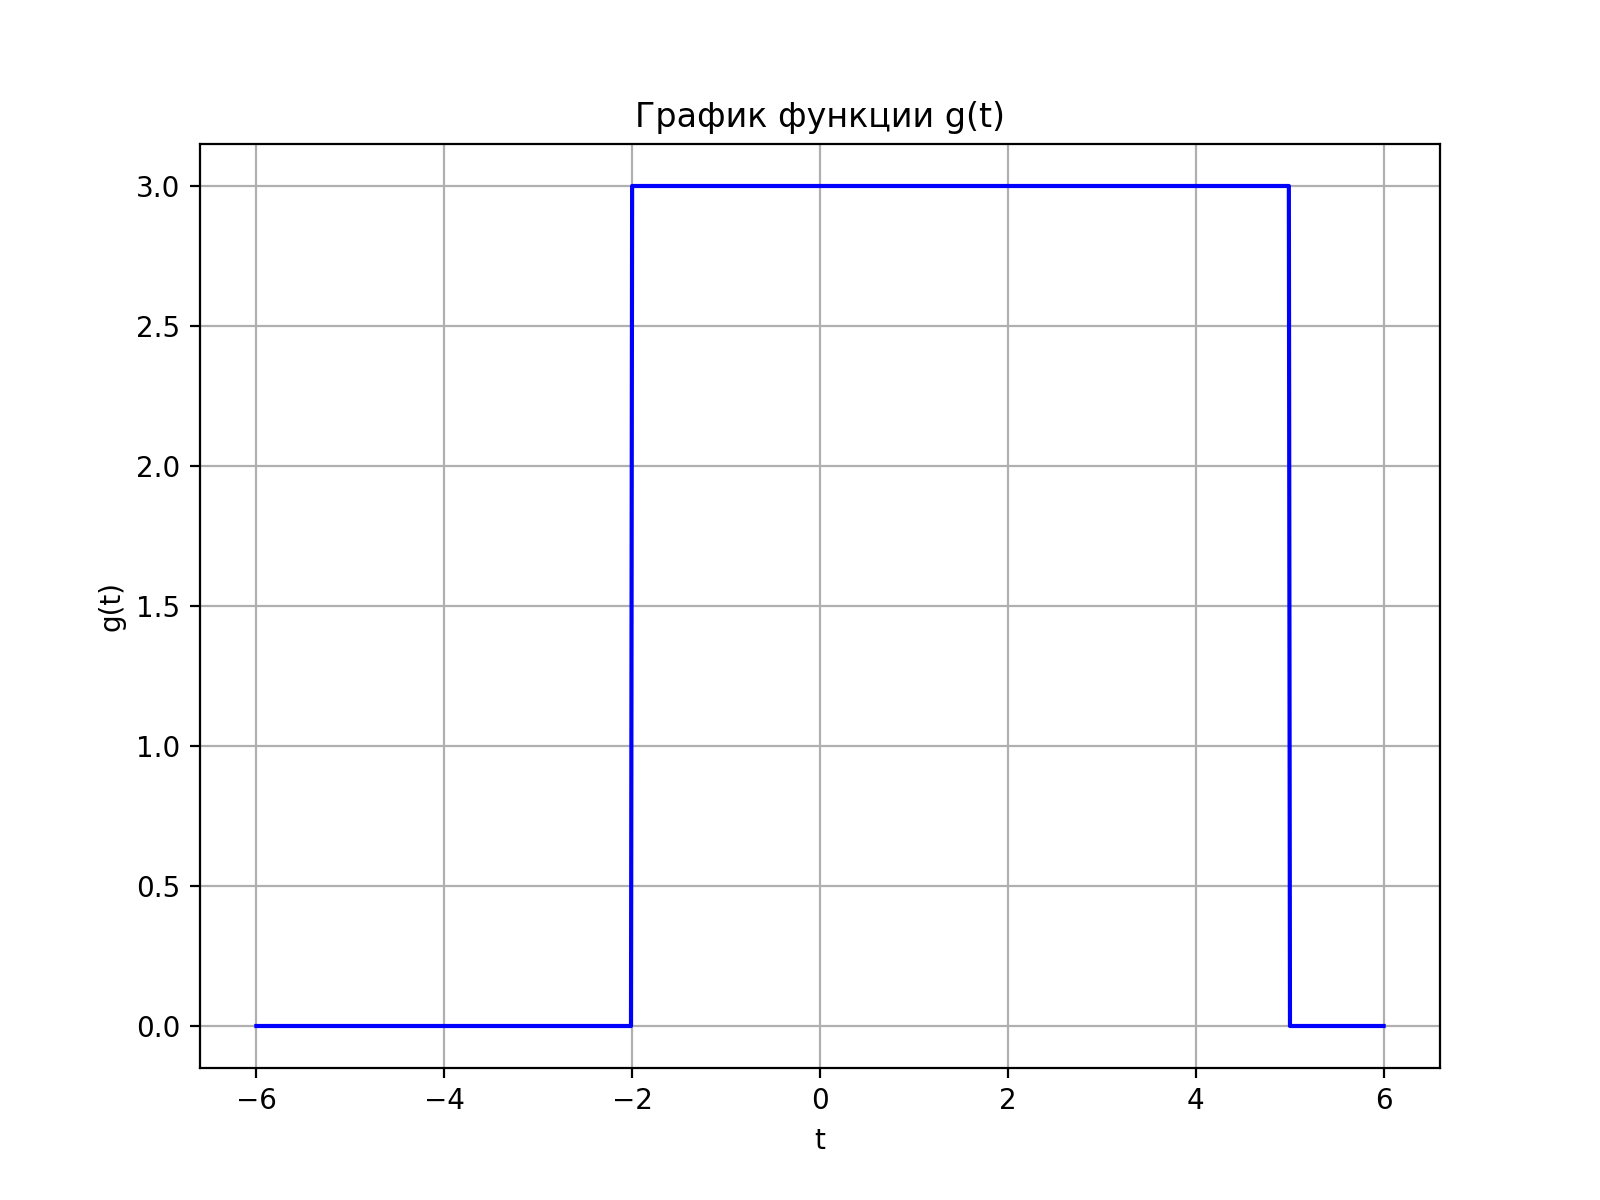
\includegraphics[width=\textwidth]{media/1 task/high_freq/Initial.png}
    \caption{График функции $g(t)$}
    \label{fig:initial}
\end{figure}

\clearpage

Для выполнения первого задания нам необходимо создать зашумлённую версию функции, или сигнала, при помощи функции

\begin{equation}
    u(t)=g(t)+b(rand(size(t))-0.5)+c*\sin(d*t),
\end{equation}

в которой $b$, $c$, $d$ - параметры, чьё влияние на фильтрацию сигнала $u(t)$ мы будем исследовать в этом задании.

\subsection{Высокие частоты}\label{high_freq}

При выполнении этого пункта значение параметра $c$ мы примем равным $0$. Параметр $b$ принимает значения $0.25, 1, 4$. Графики зашумлённого сигнала приведены ниже:

\begin{figure}[ht!]
    \centering
    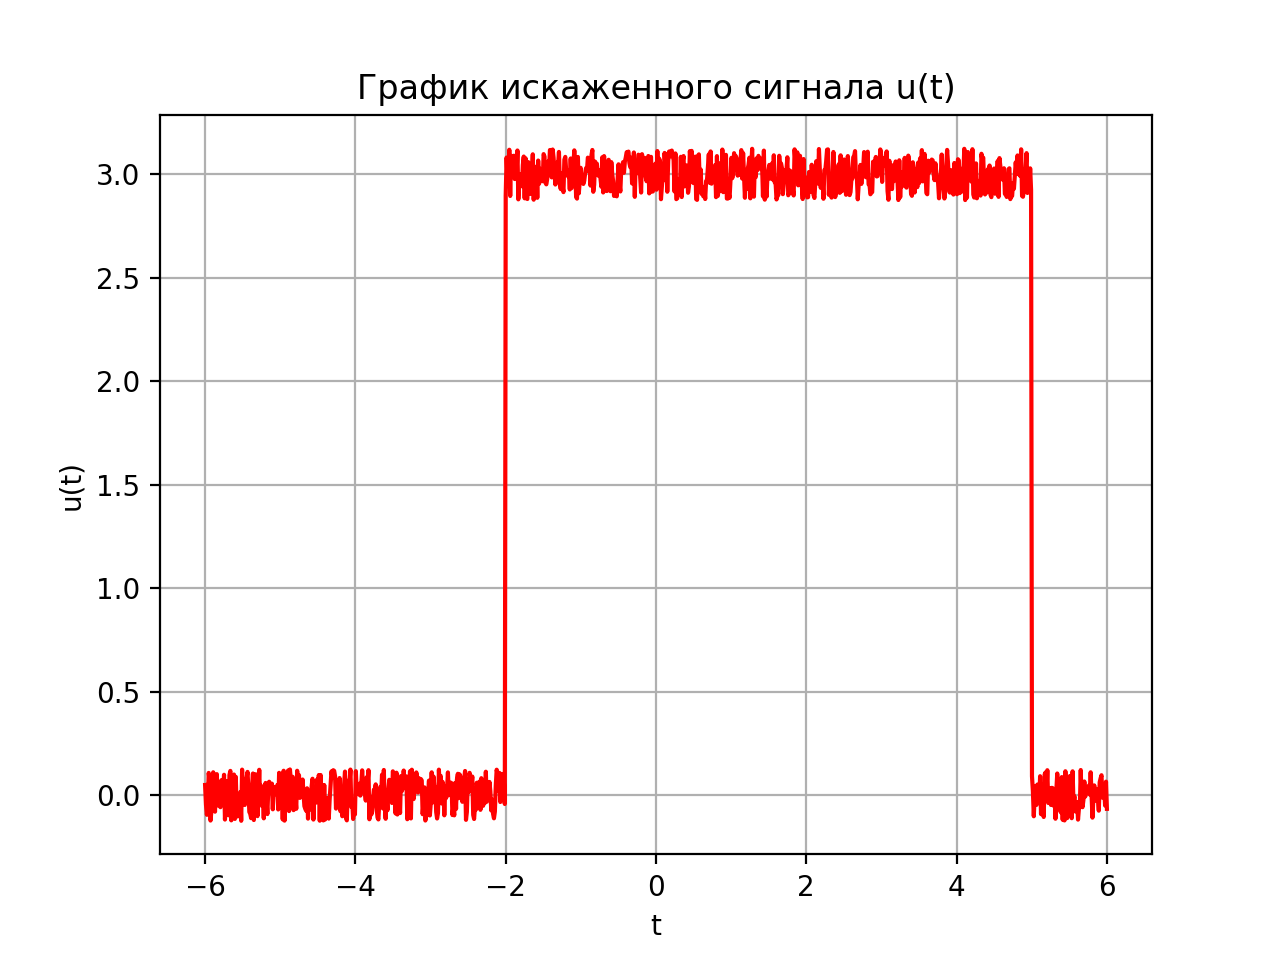
\includegraphics[scale=0.75]{media/1 task/high_freq/Noisy_0,25.png}
    \caption{График функции $u(t)$ при $b=0.25$}
    \label{fig:noisy_025}
\end{figure}

\clearpage

\begin{figure}[ht!]
    \centering
    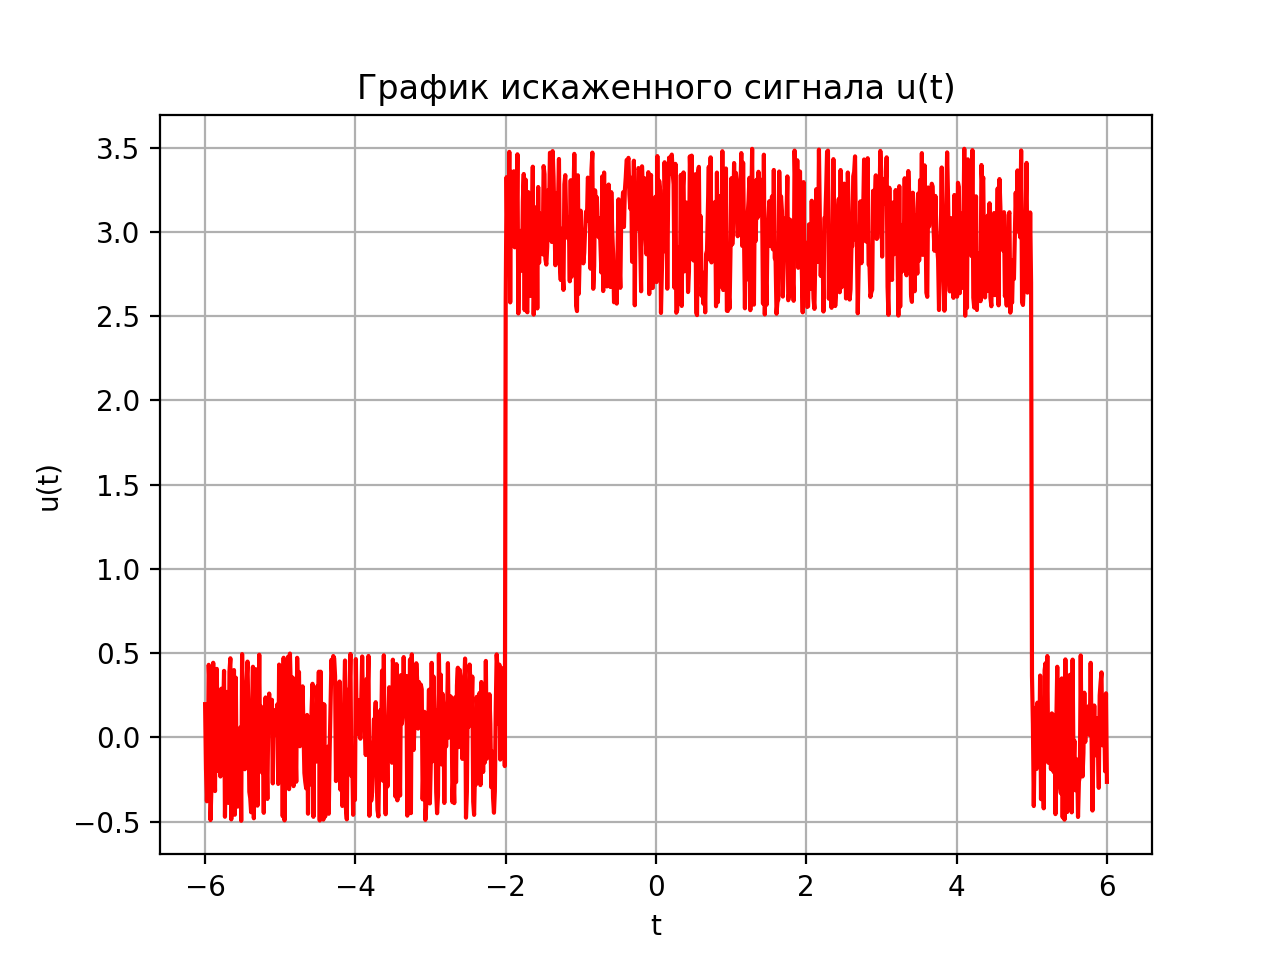
\includegraphics[scale=0.75]{media/1 task/high_freq/Noisy_1.png}
    \caption{График функции $u(t)$ при $b=1$}
    \label{fig:noisy_1}
\end{figure}

\begin{figure}[ht!]
    \centering
    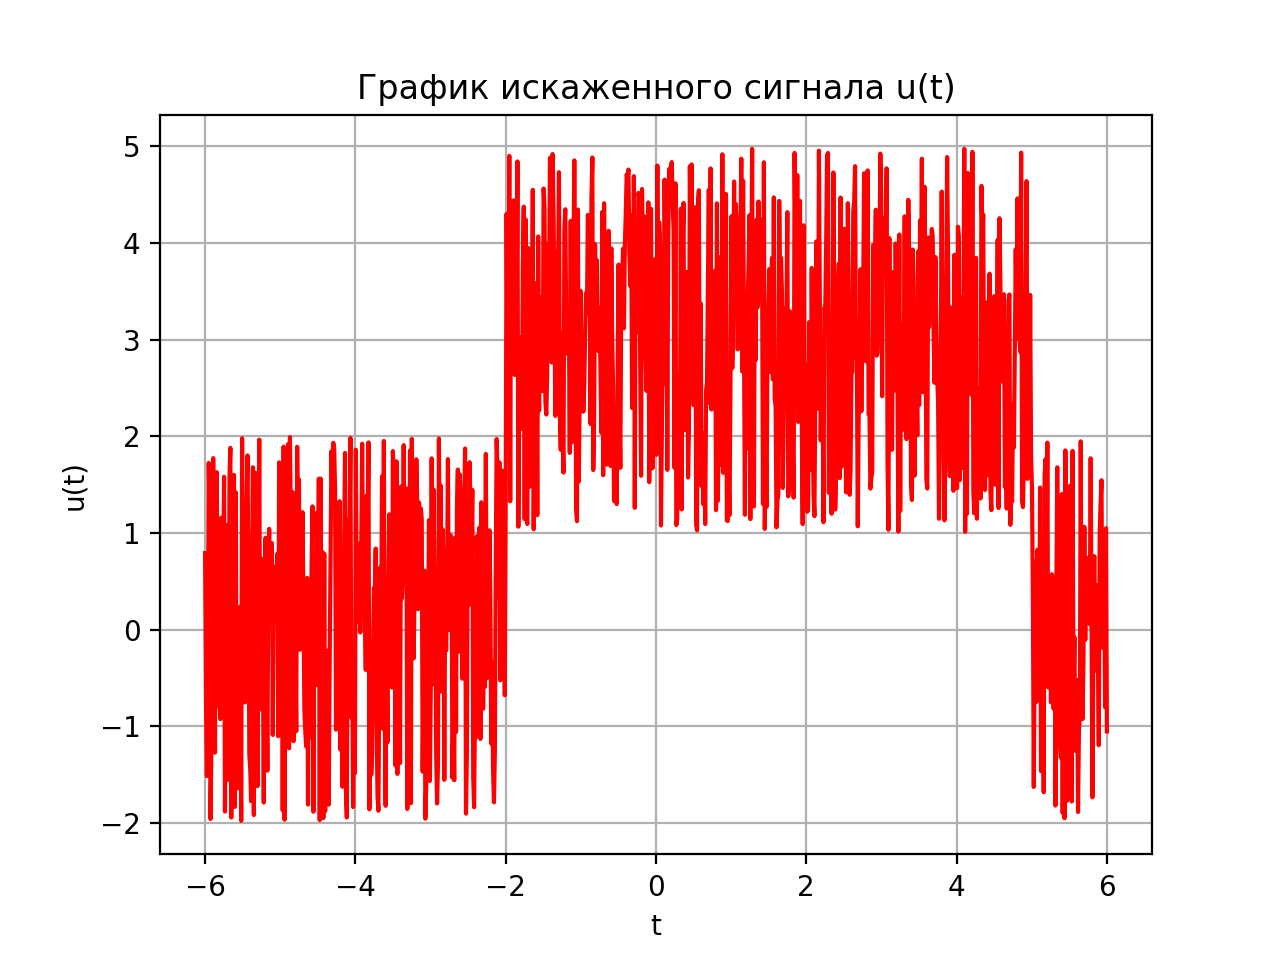
\includegraphics[scale=0.75]{media/1 task/high_freq/Noisy_4.png}
    \caption{График функции $u(t)$ при $b=4$}
    \label{fig:noisy_4}
\end{figure}

Благодаря графикам мы можем сделать вывод о том, что параметр $b$ влияет на степень хаотического шума, точнее на его амплитуду. Переходим к фильтрации!
\subsubsection{Режем Фурье-образы и фильтруем сигнал!}
 
Снова обращаемся к замечательному Фурье-преобразованию! Для выполнения задания 1 будем выполнять его для частоты $\nu$. В качестве частот среза ($\nu_0$) будут выступать значения $0.6, 1.2, 1.8$ Гц. Построим графики модулей Фурье-образов сигнала $u(t)$ и отфильтрованного сигнала, а также сравнительные графики модулей $g(t)$ и отфильтрованного сигнала:

\begin{figure}[ht!]
    \centering
    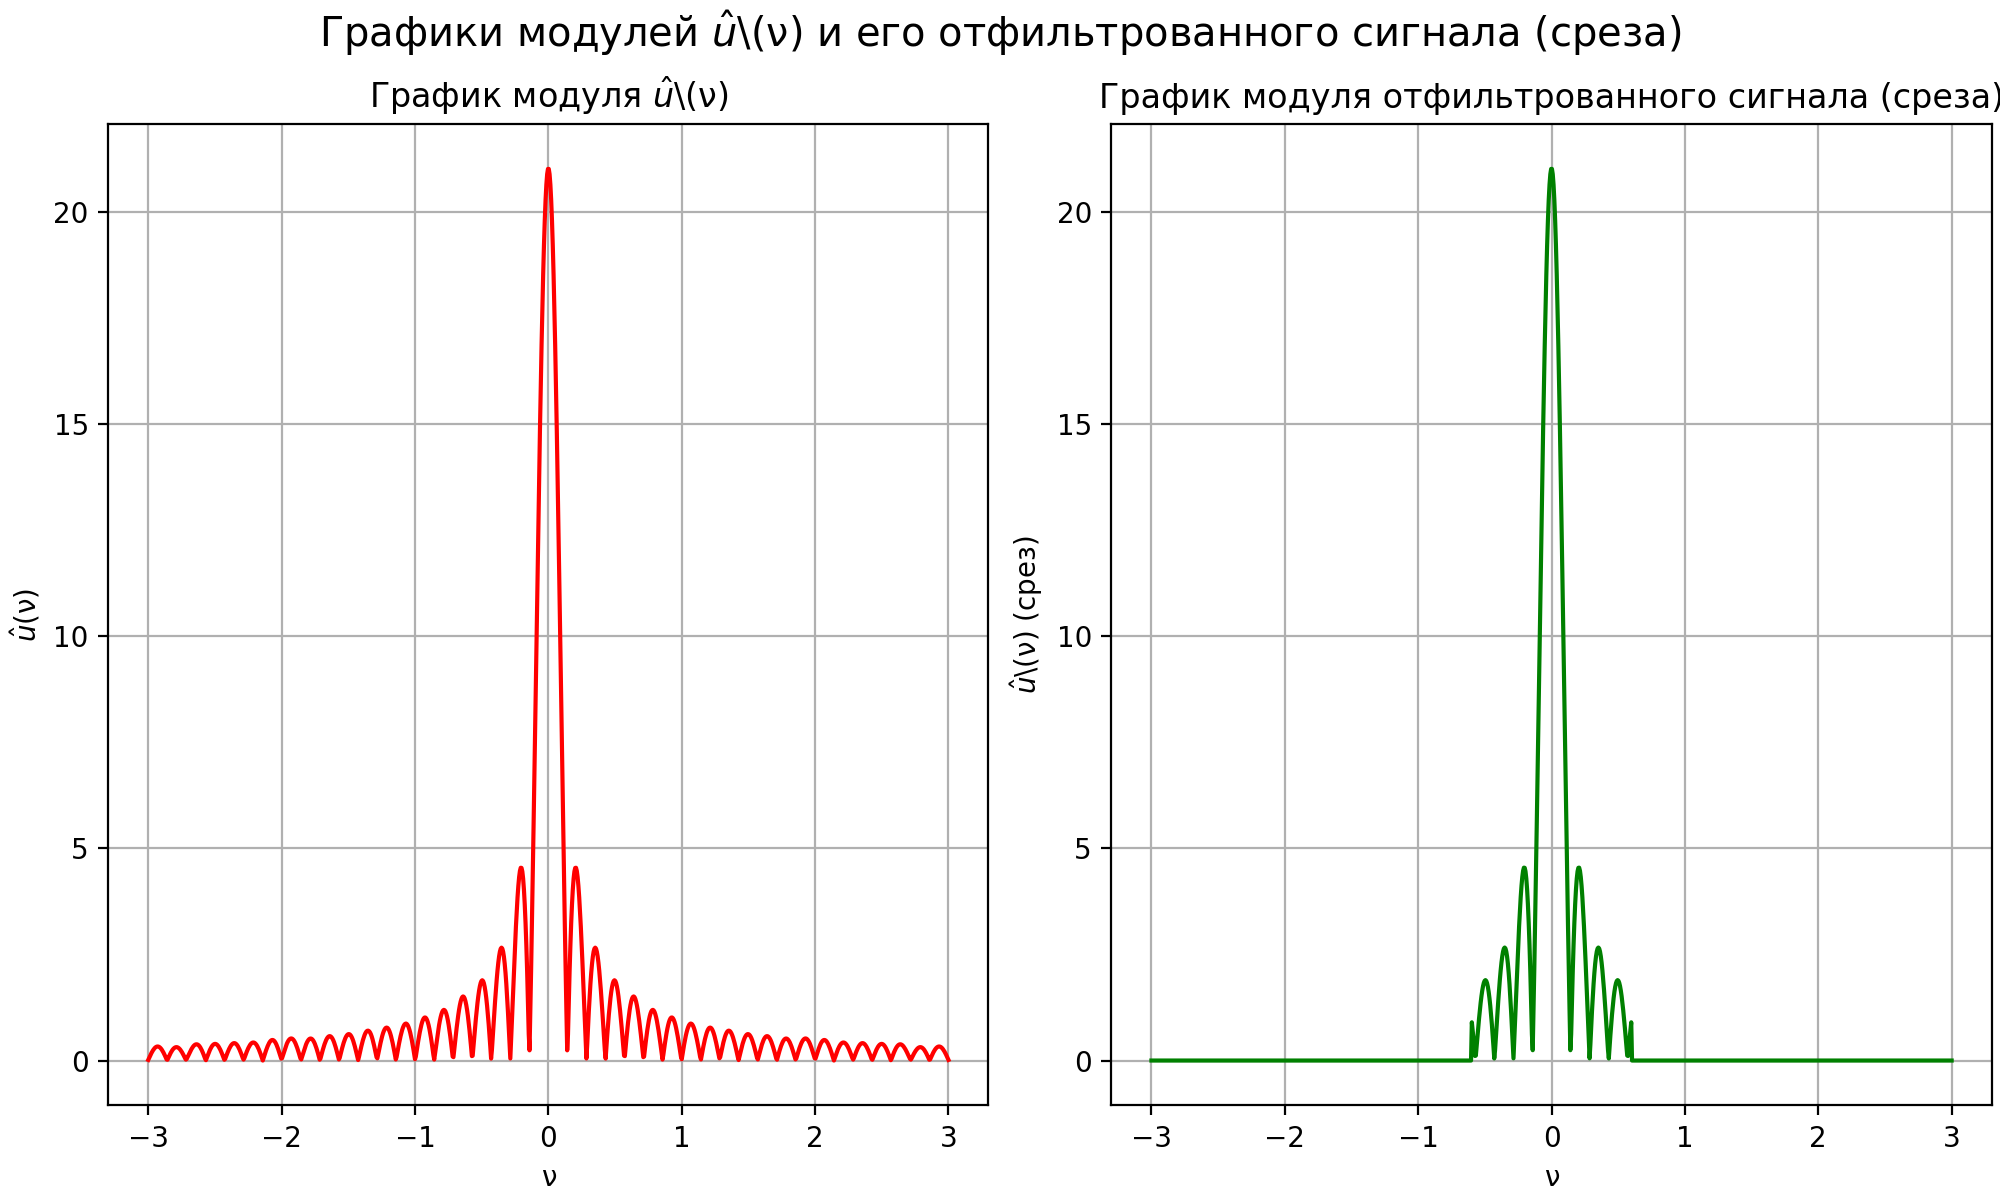
\includegraphics[scale=0.55]{media/1 task/high_freq/Fourier_Image_0,25_-0,5975975975975976.png}
    \caption{Графики модулей Фурье-образа $u(t)$ и отфильтрованного сигнала при $b=0.25$ и $\nu_0=0.6$ Гц}
    \label{fig:four_025_06}
\end{figure}

\begin{figure}[ht!]
    \centering
    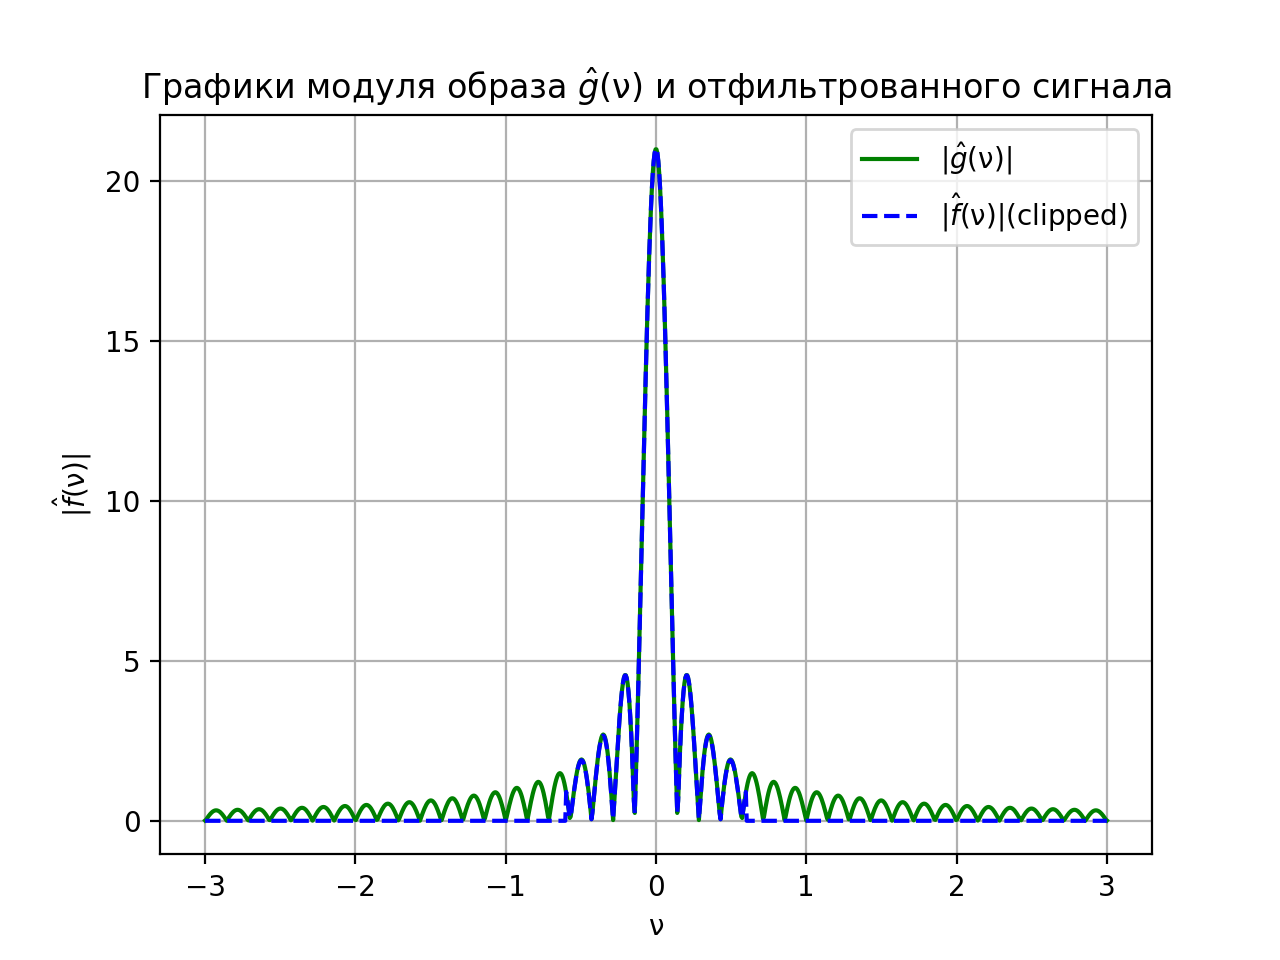
\includegraphics[scale=0.55]{media/1 task/high_freq/Fourier_Image_Comparison_0,25_-0,5975975975975976.png}
    \caption{Сравнительные графики модулей Фурье-образа $g(t)$ и отфильтрованного сигнала при $b=0.25$ и $\nu_0=0.6$ Гц}
    \label{fig:fourc_025_06}
\end{figure}

\begin{figure}[ht!]
    \centering
    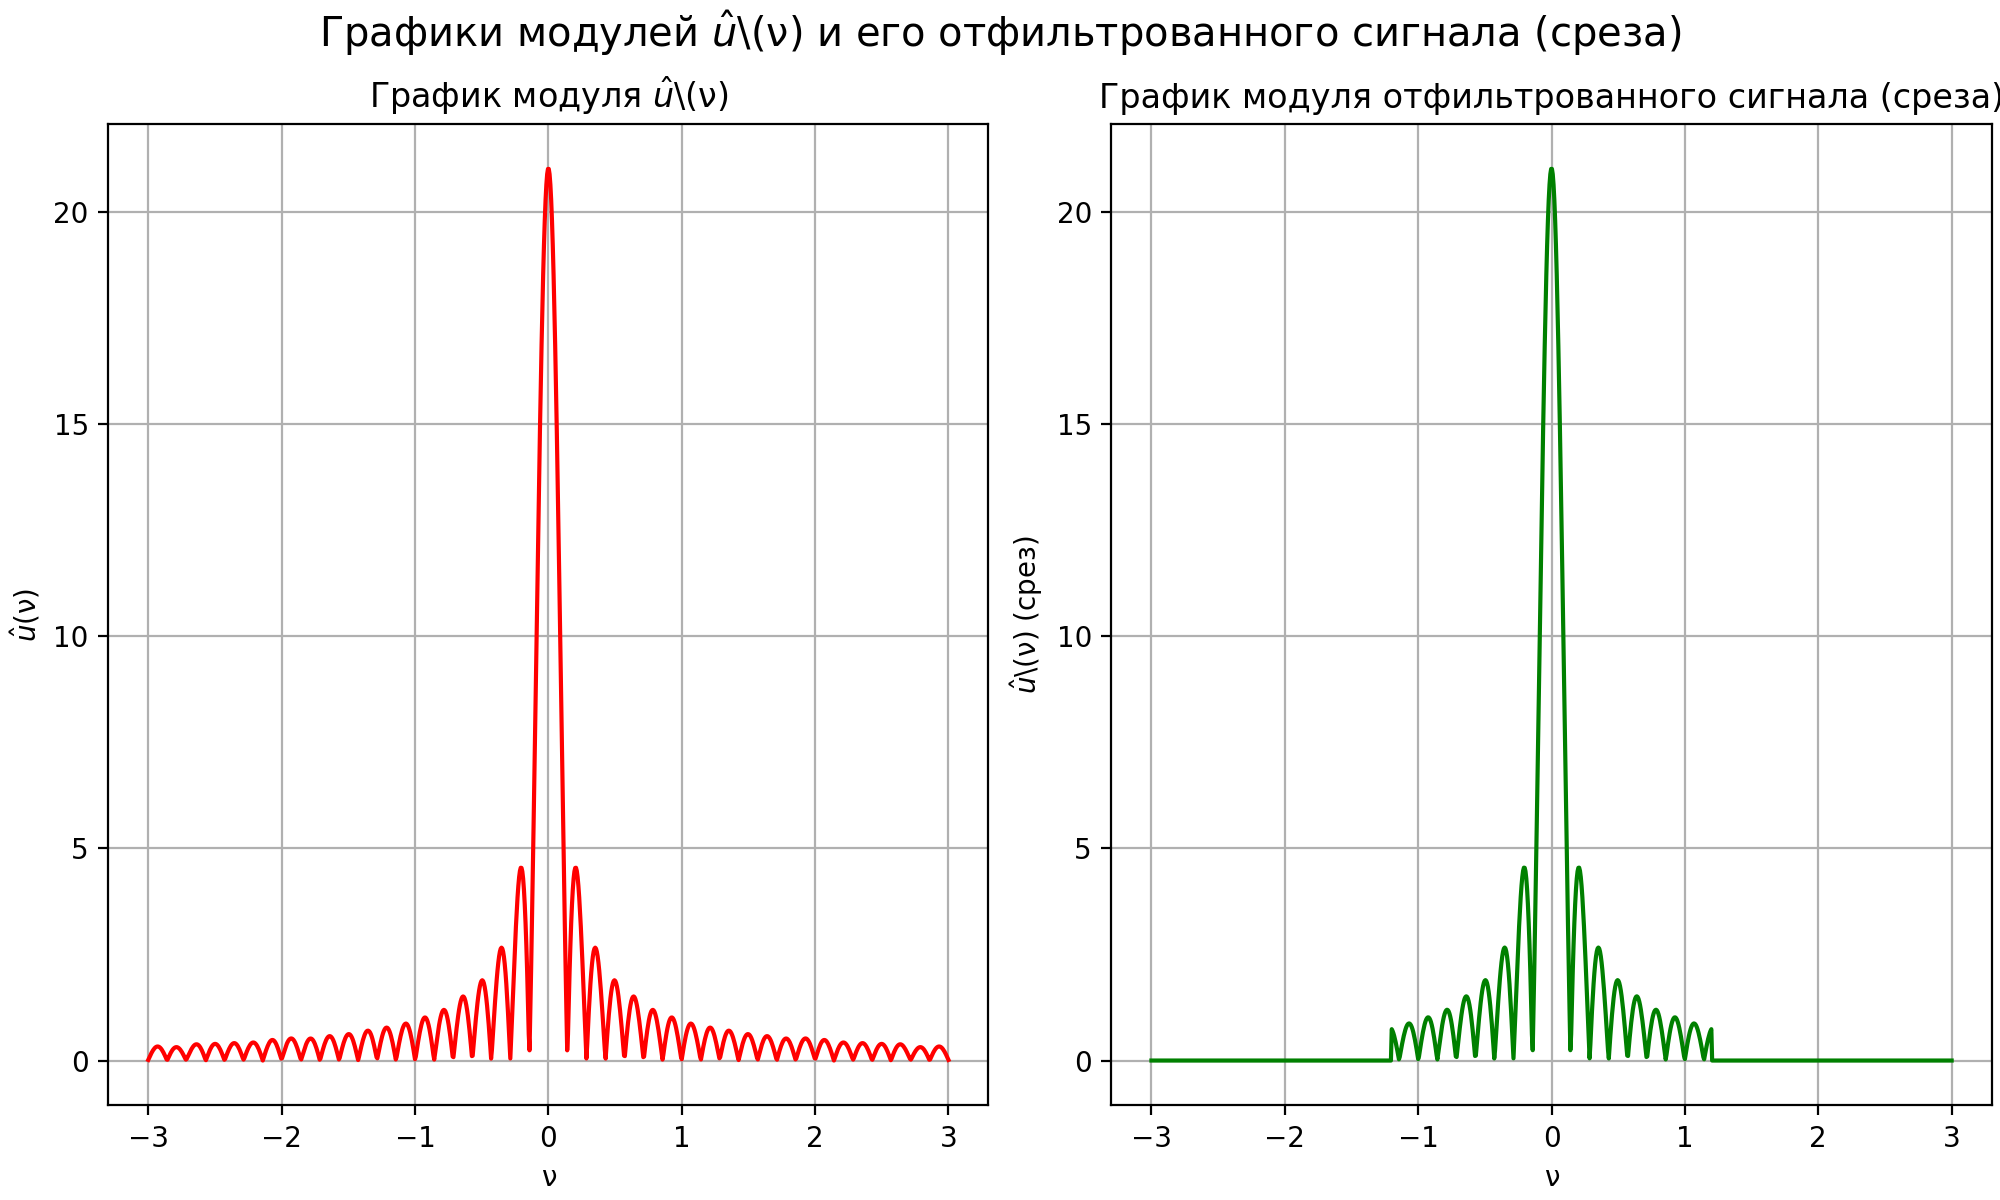
\includegraphics[scale=0.55]{media/1 task/high_freq/Fourier_Image_0,25_-1,1981981981981982.png}
    \caption{Графики модулей Фурье-образа $u(t)$ и отфильтрованного сигнала при $b=0.25$ и $\nu_0=1.2$ Гц}
    \label{fig:four_025_12}
\end{figure}

\begin{figure}[ht!]
    \centering
    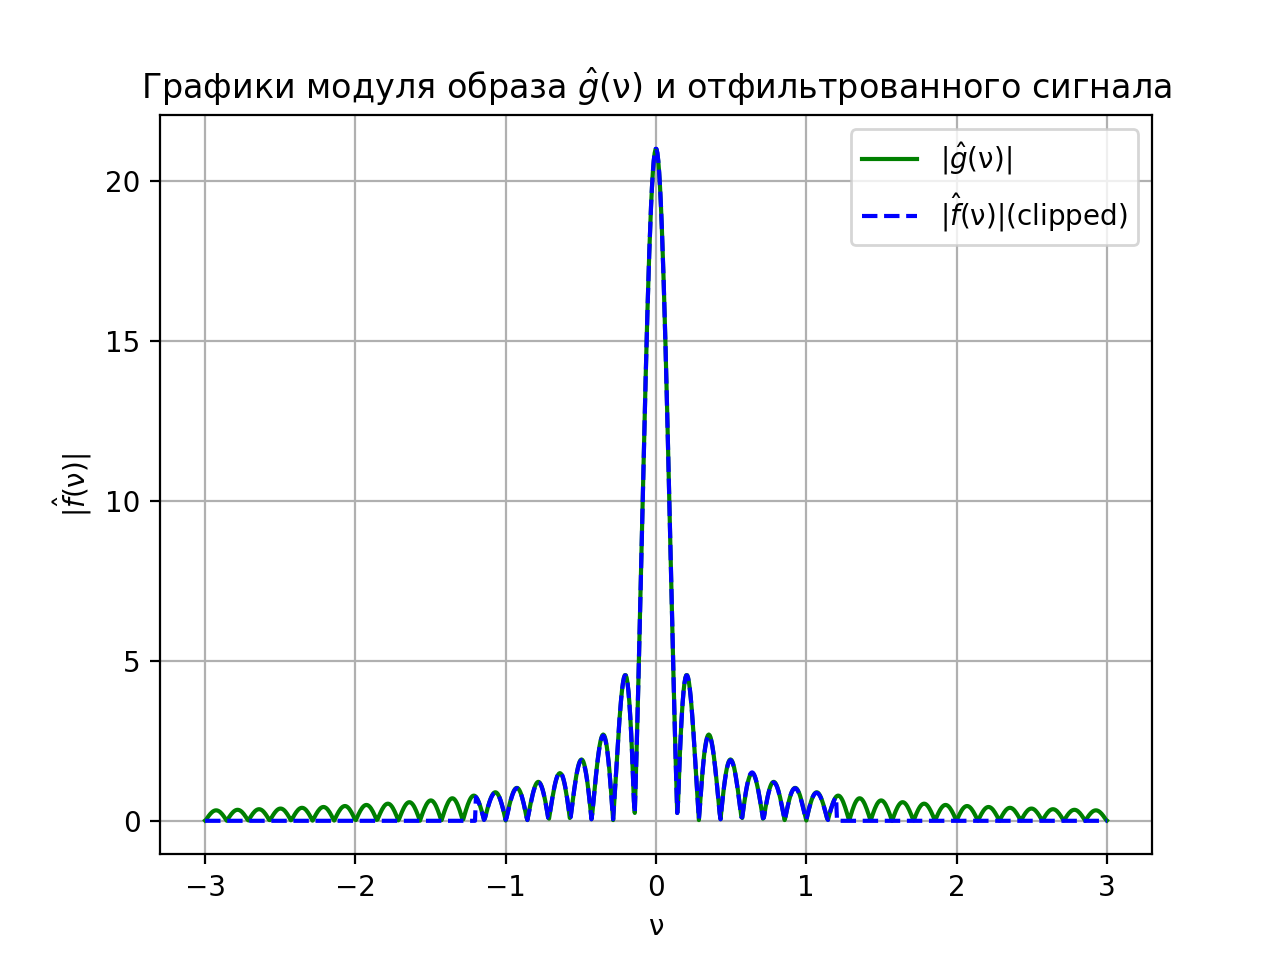
\includegraphics[scale=0.55]{media/1 task/high_freq/Fourier_Image_Comparison_0,25_-1,1981981981981982.png}
    \caption{Сравнительные графики модулей Фурье-образа $g(t)$ и отфильтрованного сигнала при $b=0.25$ и $\nu_0=1.2$ Гц}
    \label{fig:fourc_025_12}
\end{figure}

\clearpage

\begin{figure}[ht!]
    \centering
    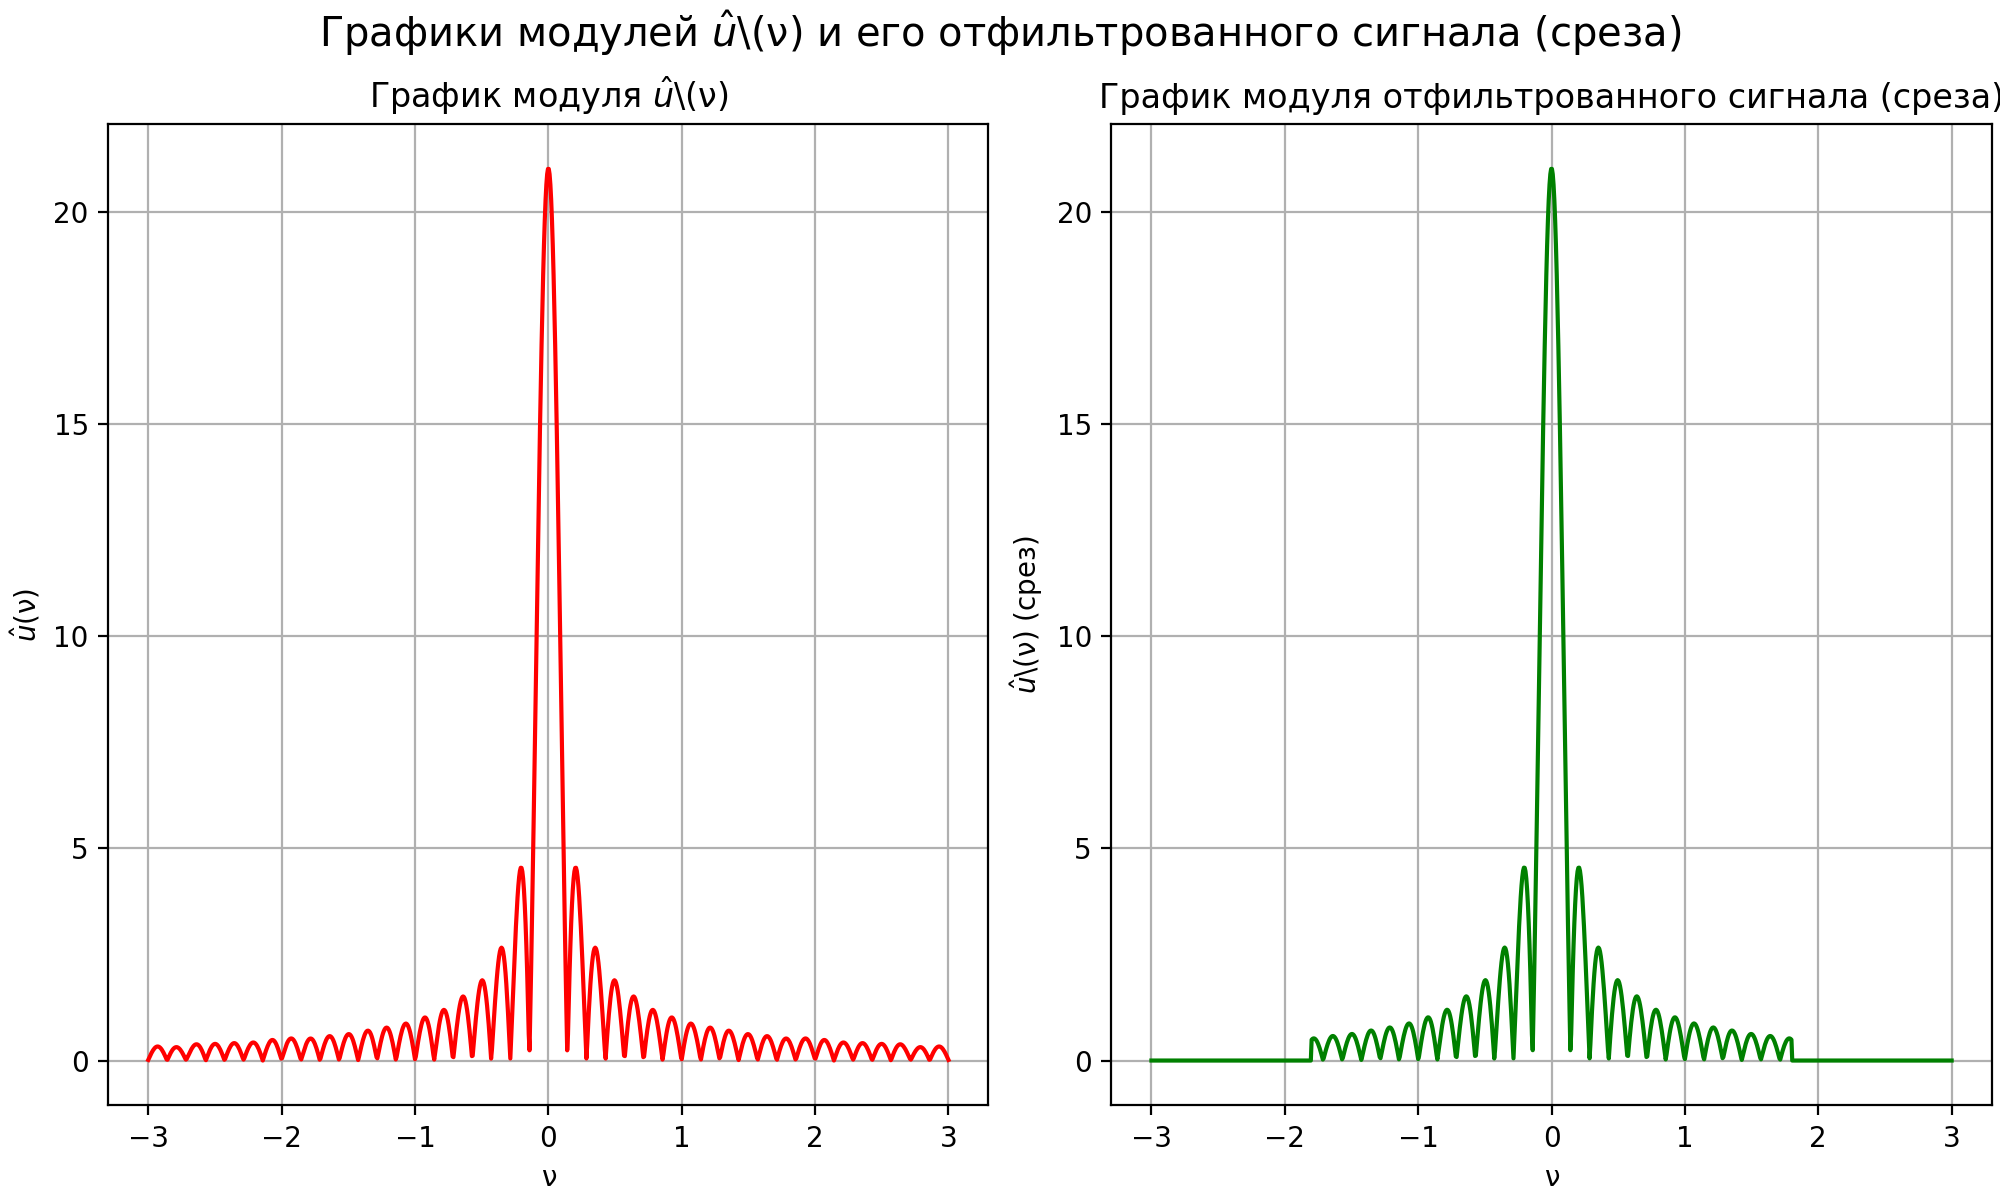
\includegraphics[scale=0.55]{media/1 task/high_freq/Fourier_Image_0,25_-1,7987987987987988.png}
    \caption{Графики модулей Фурье-образа $u(t)$ и отфильтрованного сигнала при $b=0.25$ и $\nu_0=1.8$ Гц}
    \label{fig:four_025_18}
\end{figure}

\begin{figure}[ht!]
    \centering
    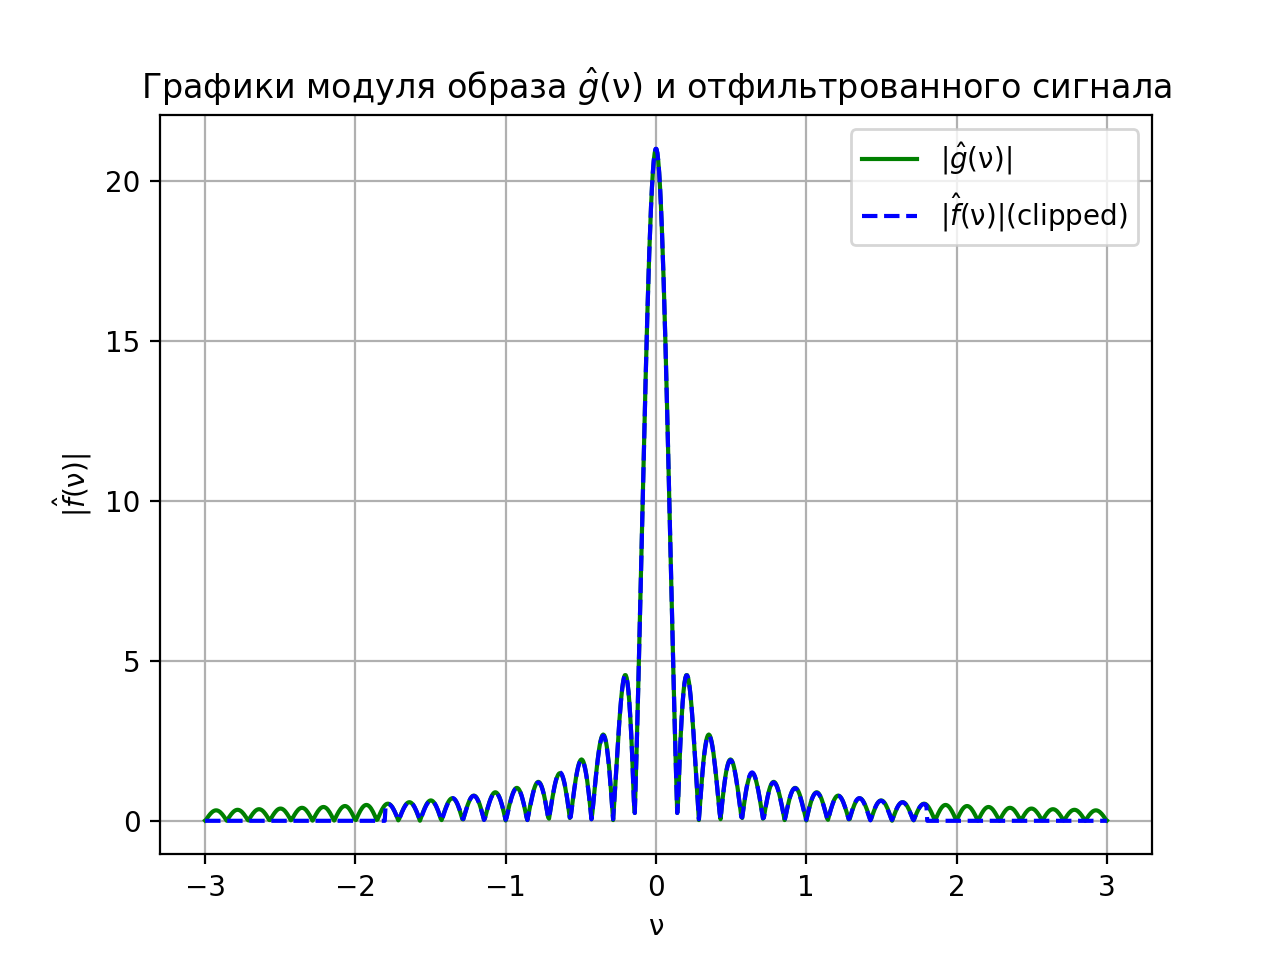
\includegraphics[scale=0.55]{media/1 task/high_freq/Fourier_Image_Comparison_0,25_-1,7987987987987988.png}
    \caption{Сравнительные графики модулей Фурье-образа $g(t)$ и отфильтрованного сигнала при $b=0.25$ и $\nu_0=1.8$ Гц}
    \label{fig:fourc_025_18}
\end{figure}

Выше были приведены графики для сигнала $u(t)$ при $b=0.25$, но с разными частотами среза. Это сделано для того, чтобы мы смогли узнать влияние частоты среза на отфильтрованный сигнал. Так что выполняем обратное преобразование Фурье <<обрезанного>> образа и сопоставляем полученный отфильтрованный сигнал с зашумленным и исходным:

\clearpage

\begin{figure}[ht!]
    \centering
    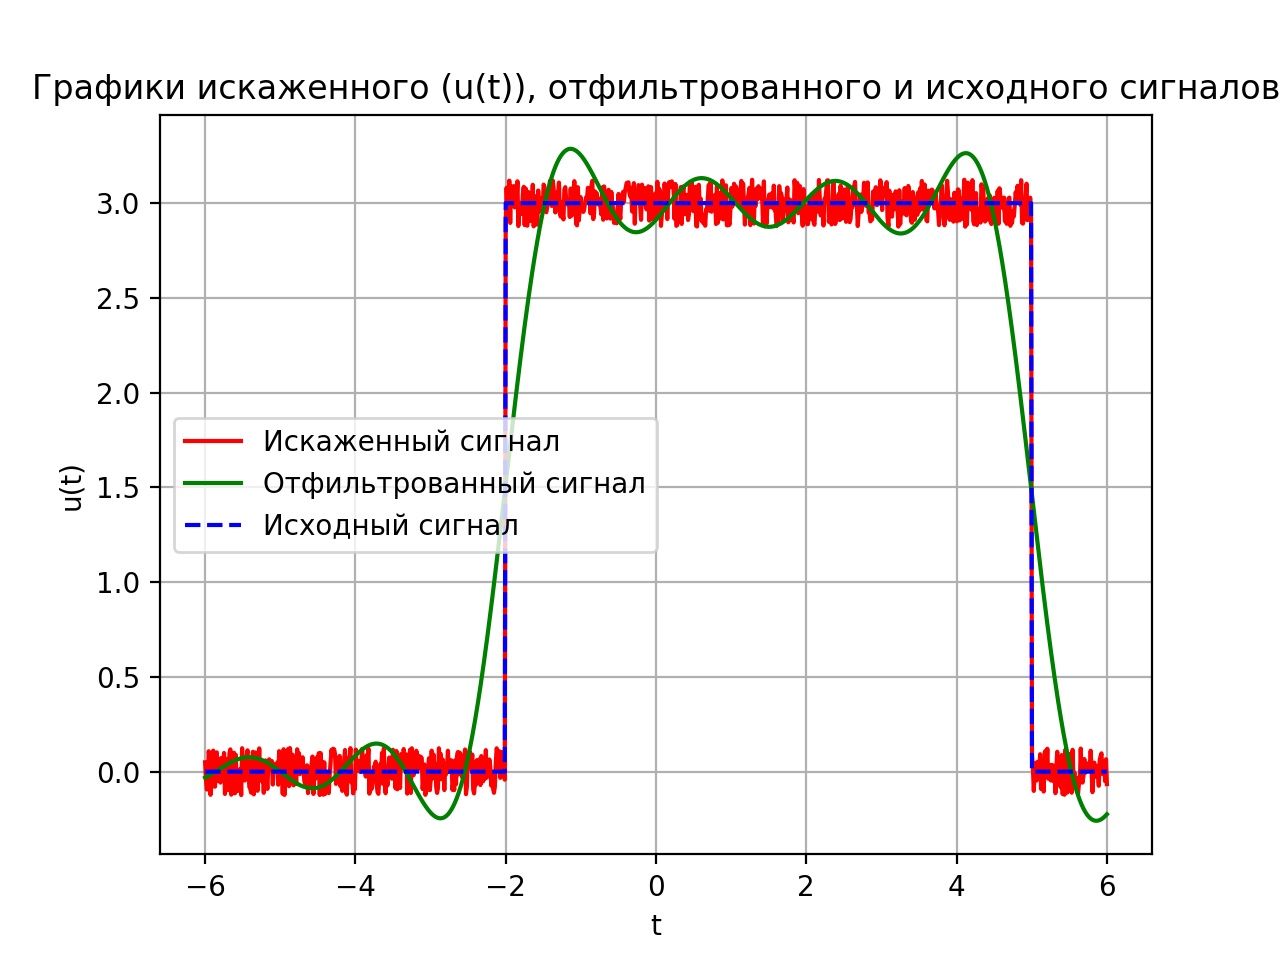
\includegraphics[scale=0.85]{media/1 task/high_freq/Cleaned_0,25_-0,5975975975975976.png}
    \caption{Графики  $u(t)$, отфильтрованного и исходного сигналов при $b=0.25$ и $\nu_0=0.6$ Гц}
    \label{fig:cleaned_025_06}
\end{figure}

\begin{figure}[ht!]
    \centering
    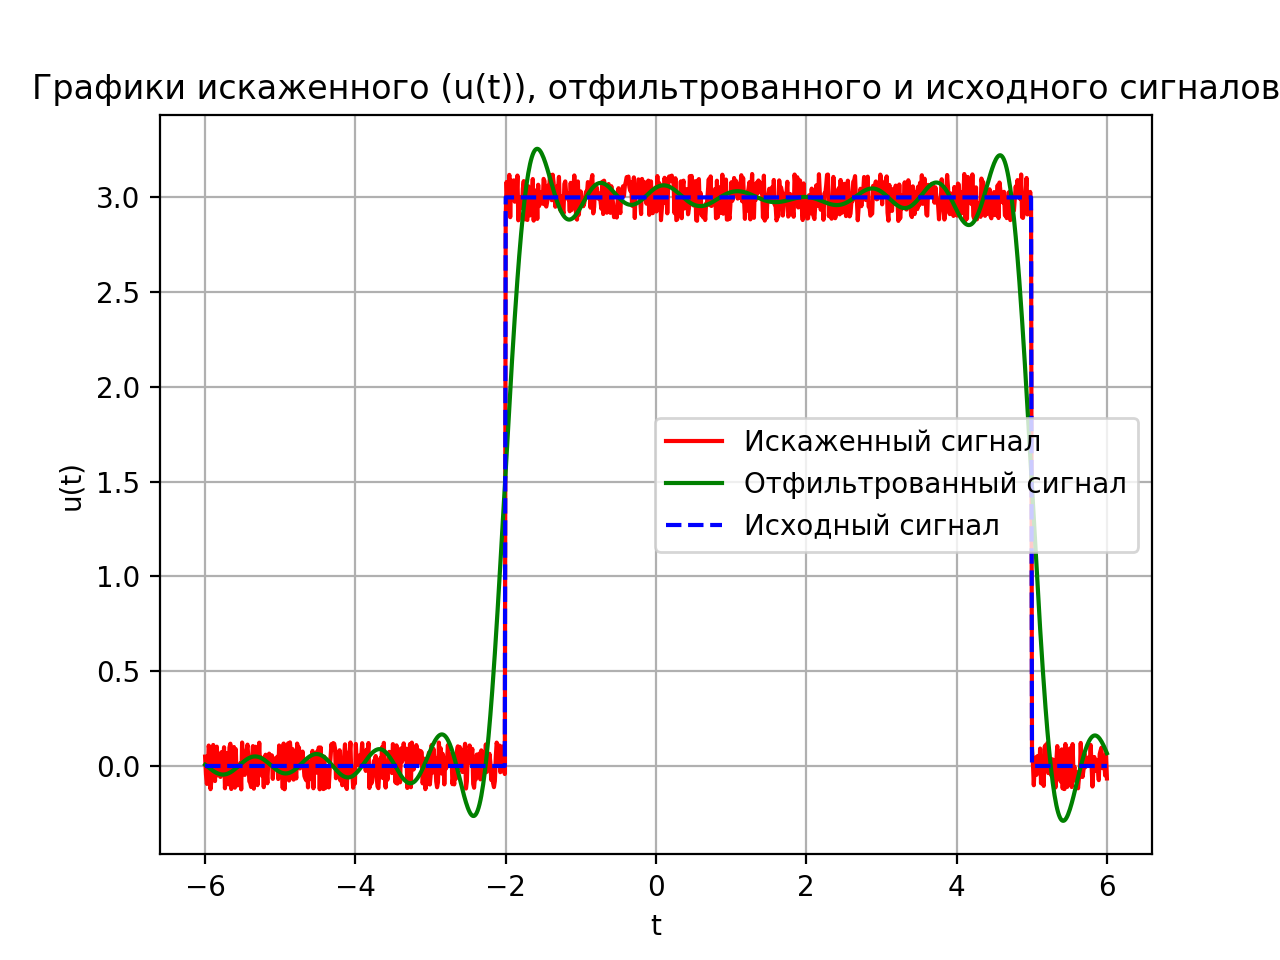
\includegraphics[scale=0.85]{media/1 task/high_freq/Cleaned_0,25_-1,1981981981981982.png}
    \caption{Графики  $u(t)$, отфильтрованного и исходного сигналов при $b=0.25$ и $\nu_0=1.2$ Гц}
    \label{fig:cleaned_025_12}
\end{figure}

\clearpage

\begin{figure}[ht!]
    \centering
    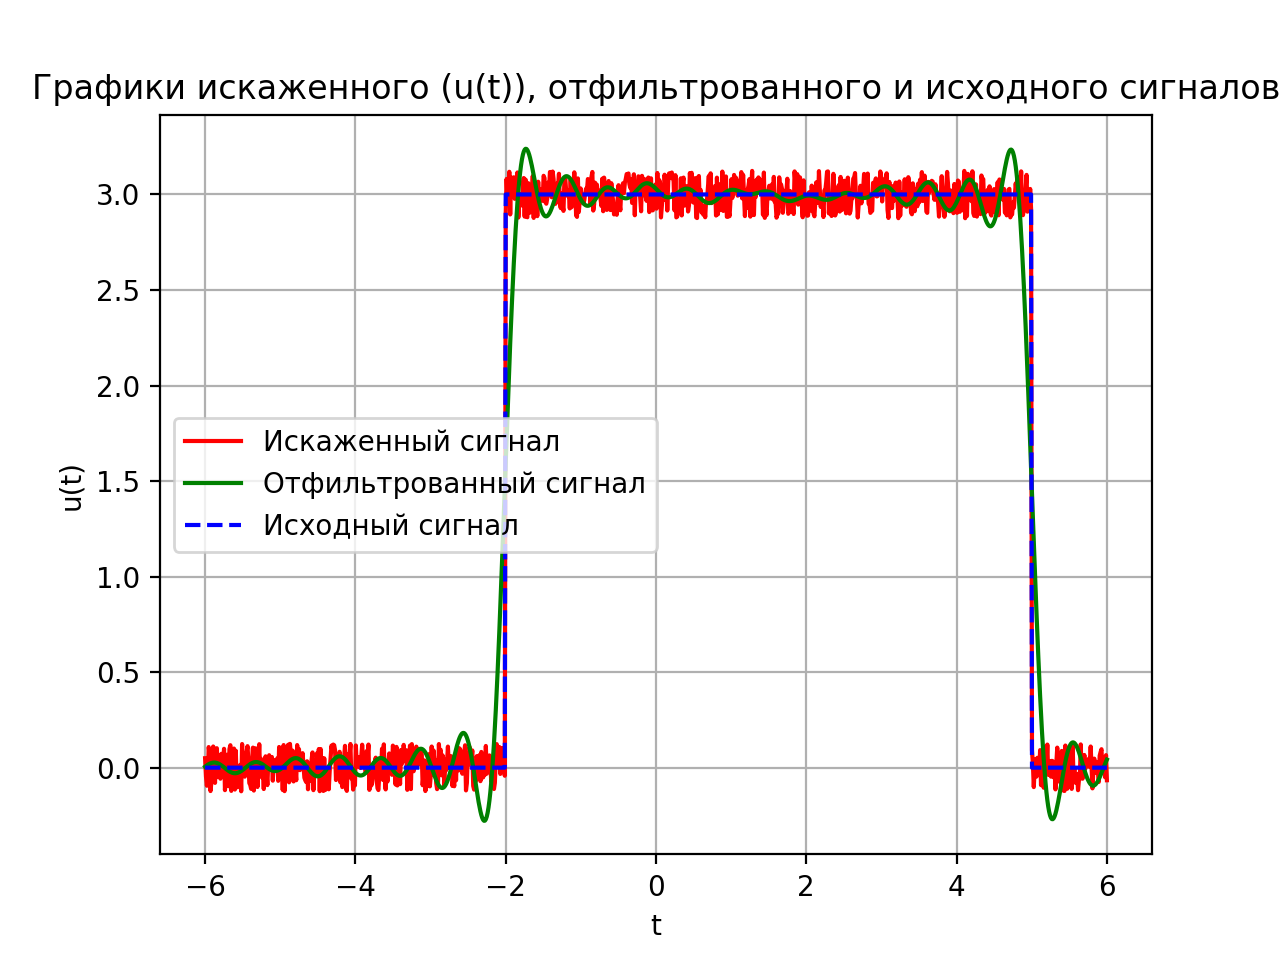
\includegraphics[scale=0.85]{media/1 task/high_freq/Cleaned_0,25_-1,7987987987987988.png}
    \caption{Графики  $u(t)$, отфильтрованного и исходного сигналов при $b=0.25$ и $\nu_0=1.8$ Гц} 
    \label{fig:cleaned_025_18}
\end{figure}

Из полученных графиков можно заключить, что при увеличении частоты среза отфильтрованный сигнал приближается к исходному по норме. В то же время увеличиваются колебания сигнала, что свидетельствует о большем влиянии хаотического шума. При меньшей частоте среза колебания (шумы) уменьшаются, но при этом функция становится более искажённой: сведение к минимуму влияния шума приводит к тому, что мы теряем часть высокочастотных компонент исходного сигнала.

Теперь зафиксируем частоту среза $\nu_0=1.2$ Гц и проанализируем влияние параметра $b$ на фильтрацию сигнала. Строим графики модулей Фурье-образов сигнала $u(t)$ и отфильтрованного сигнала, а также сравнительные графики модулей $g(t)$ и отфильтрованного сигнала при разных значениях $b$:



\begin{figure}[ht!]
    \centering
    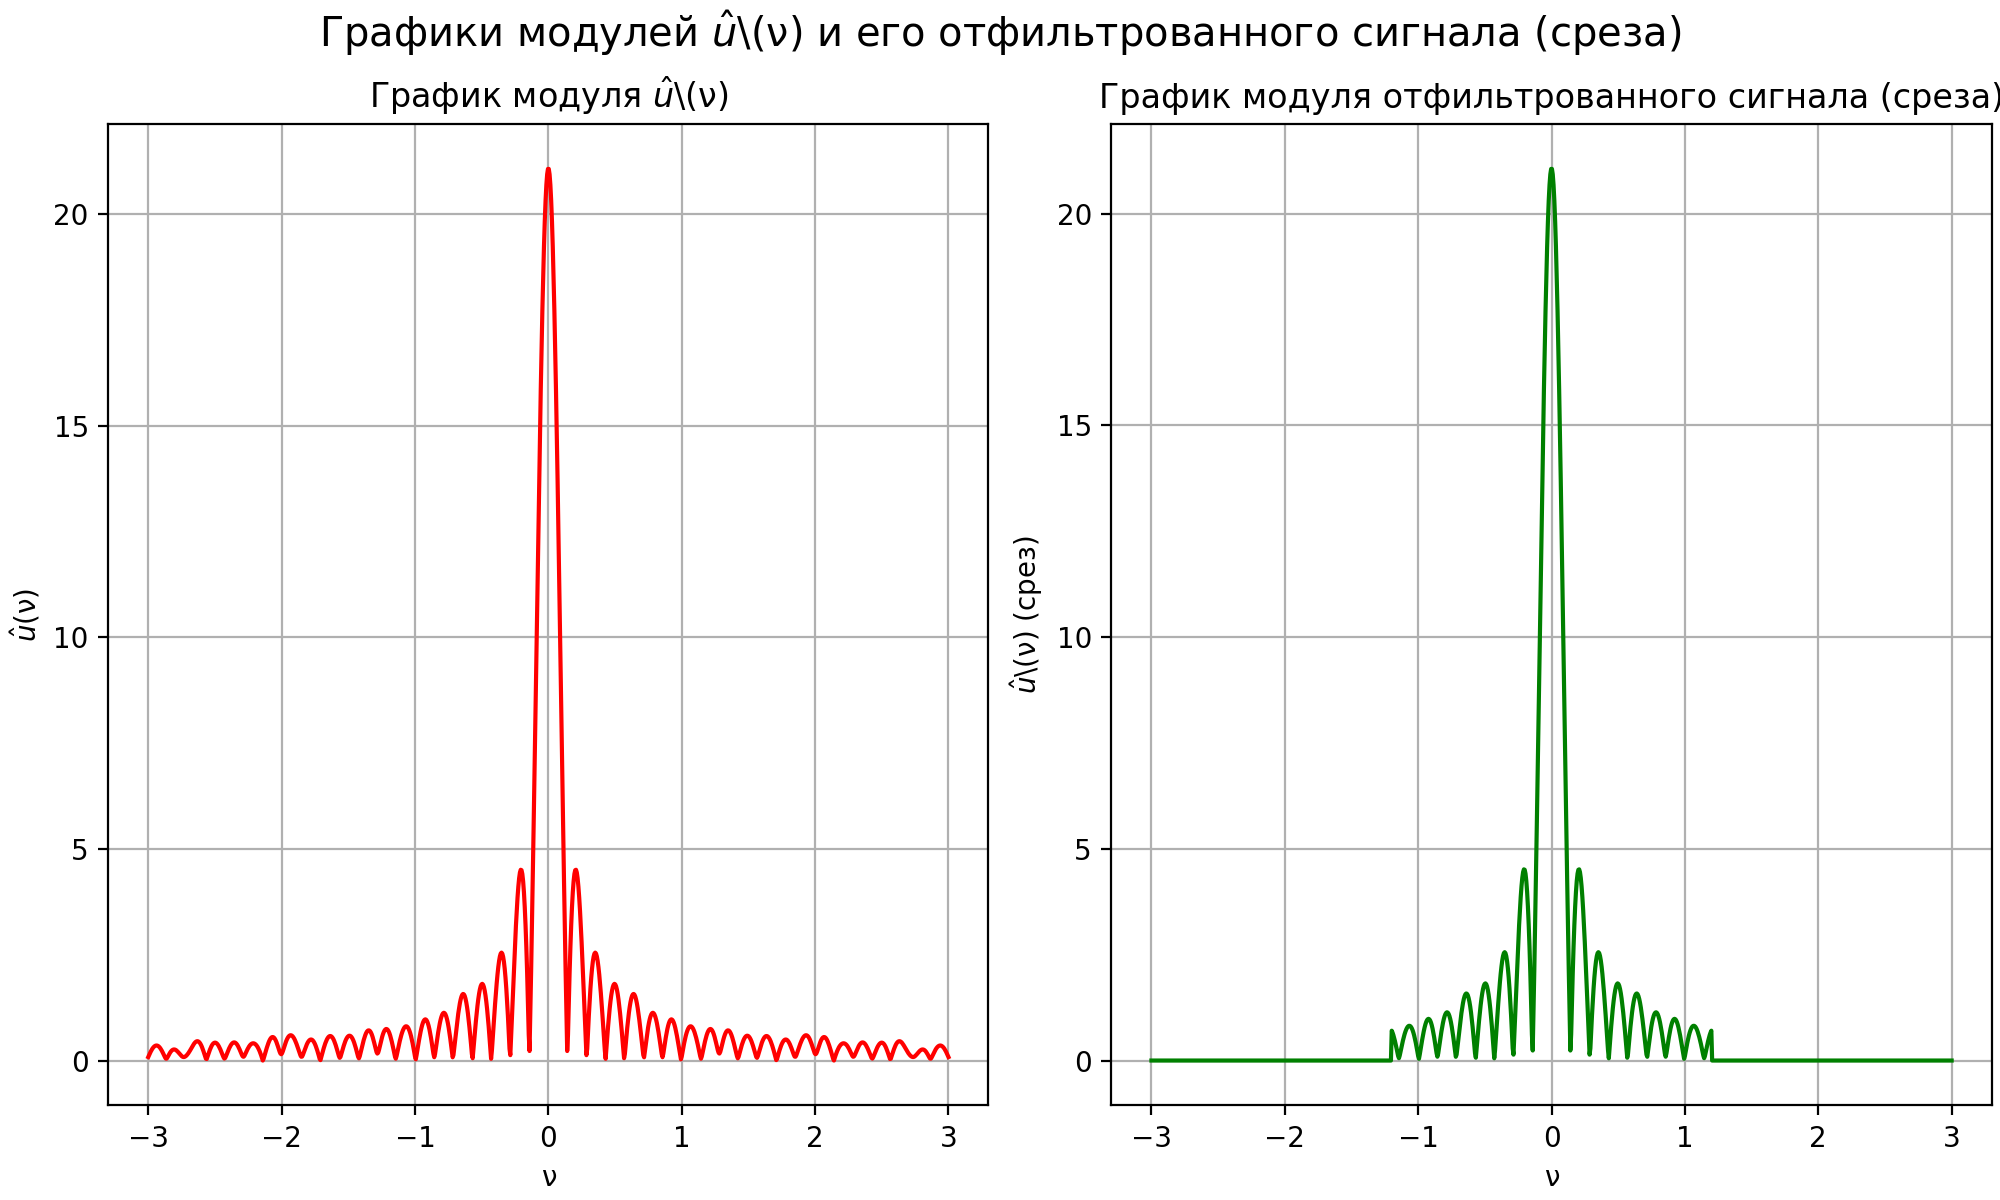
\includegraphics[scale=0.55]{media/1 task/high_freq/Fourier_Image_1_-1,1981981981981982.png}
    \caption{Графики модулей Фурье-образа $u (t)$ и отфильтрованного сигнала при $b=1$ и $\nu_0=1.2$ Гц}
    \label{fig:four_1_12}
\end{figure}

\begin{figure}[ht!]
    \centering
    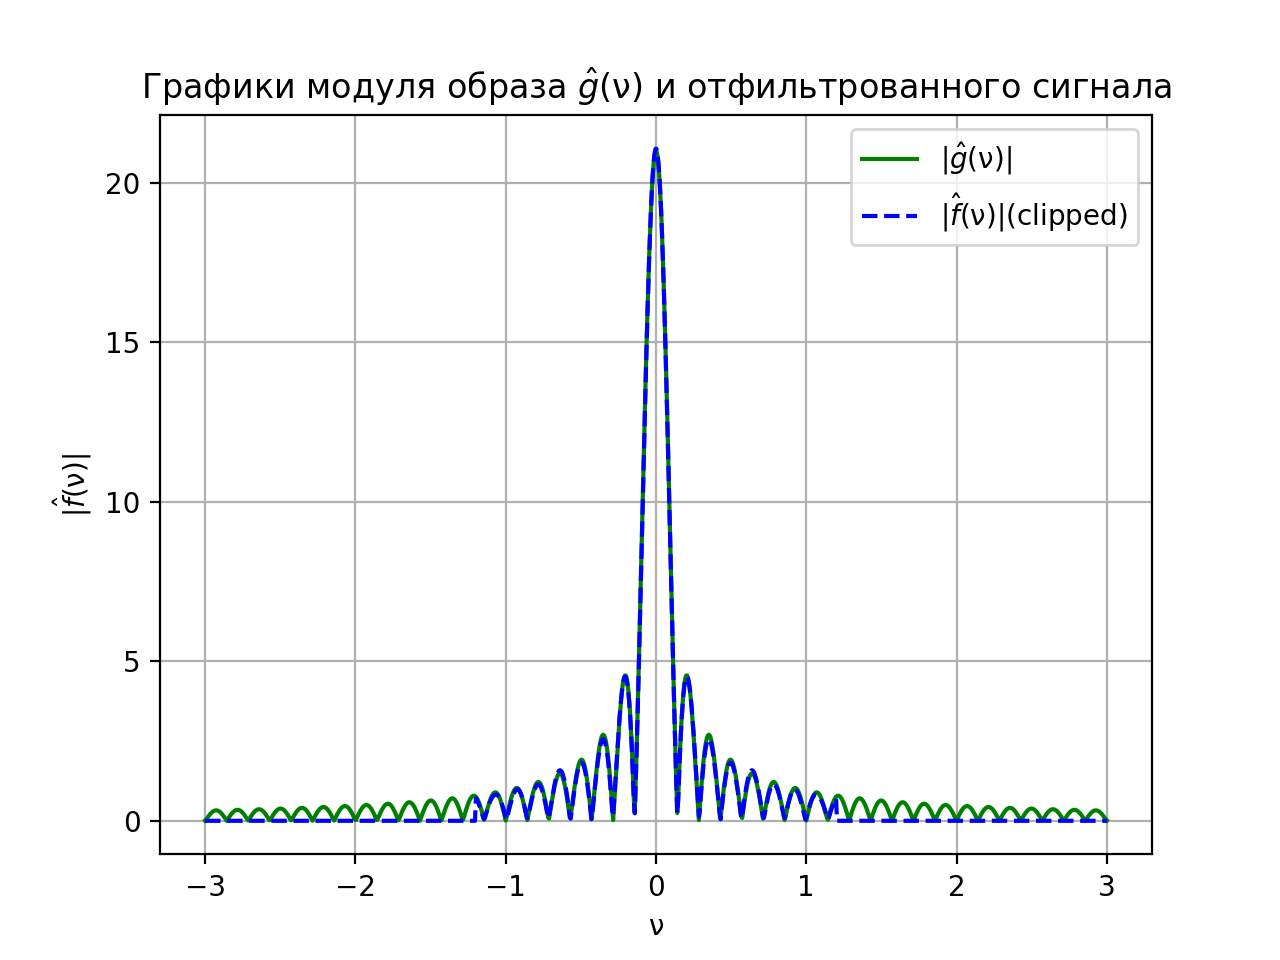
\includegraphics[scale=0.55]{media/1 task/high_freq/Fourier_Image_Comparison_1_-1,1981981981981982.png}
    \caption{Сравнительные графики модулей Фурье-образа $g(t)$ и отфильтрованного сигнала при $b=1$ и $\nu_0=1.2$ Гц}
    \label{fig:fourc_1_12}
\end{figure}

\begin{figure}[ht!]
    \centering
    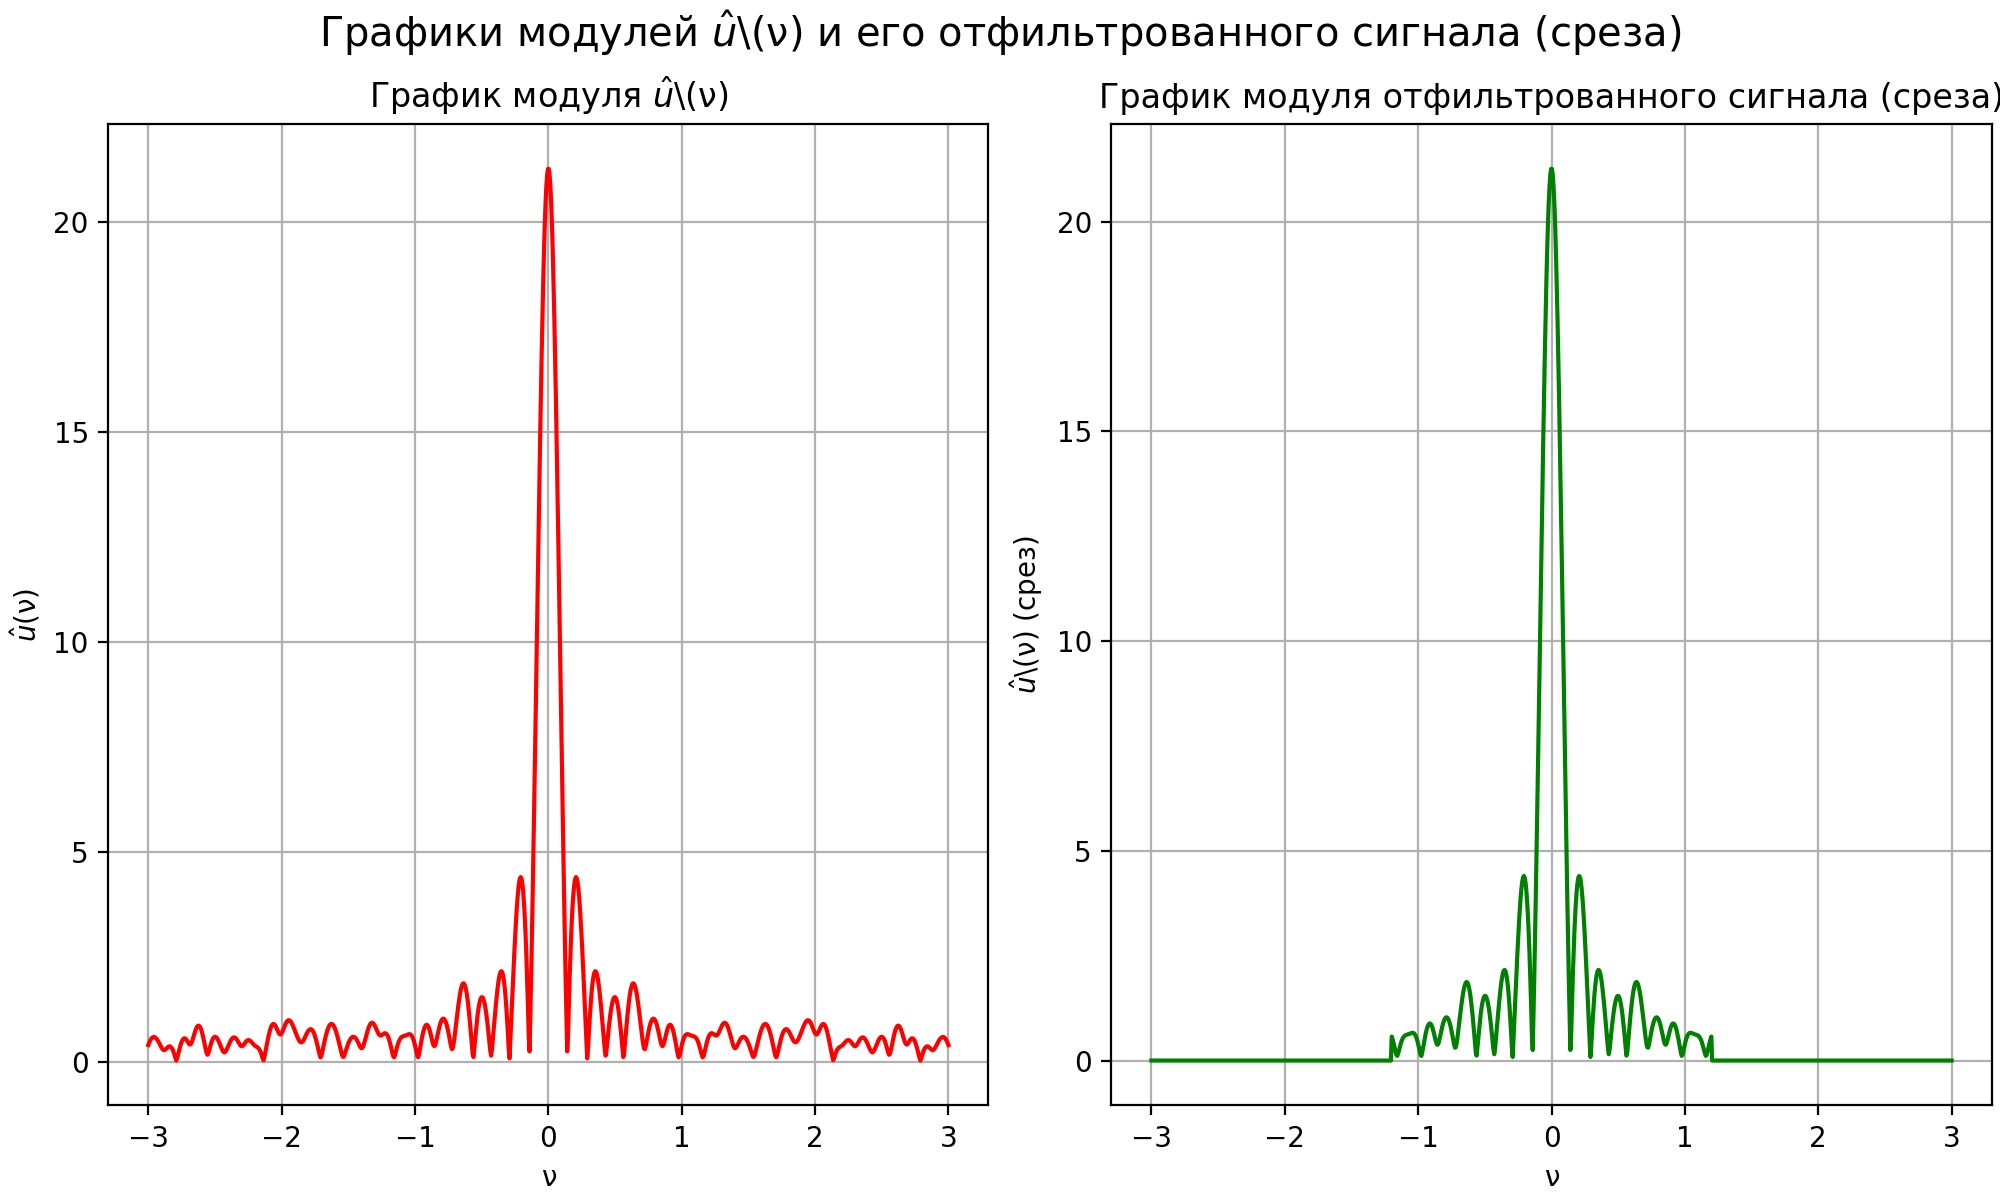
\includegraphics[scale=0.55]{media/1 task/high_freq/Fourier_Image_4_-1,1981981981981982.png}
    \caption{Графики модулей Фурье-образа $u(t)$ и отфильтрованного сигнала при $b=4$ и $\nu_0=1.2$ Гц}
    \label{fig:four_4_12}
\end{figure}

\begin{figure}[ht!]
    \centering
    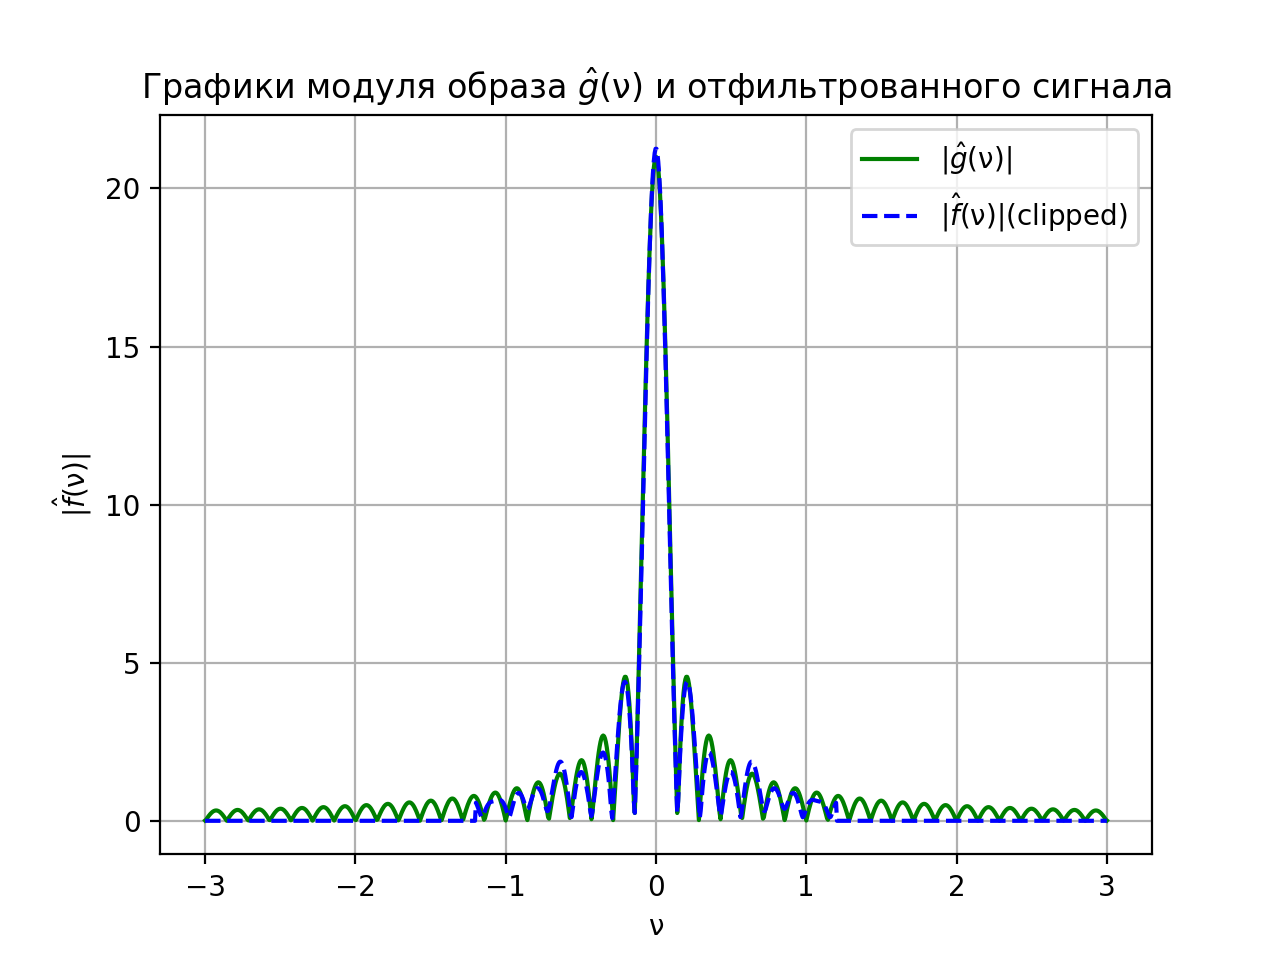
\includegraphics[scale=0.55]{media/1 task/high_freq/Fourier_Image_Comparison_4_-1,1981981981981982.png}
    \caption{Сравнительные графики модулей Фурье-образа $g(t)$ и отфильтрованного сигнала при $b=4$ и $\nu_0=1.2$ Гц}
    \label{fig:fourc_4_12}
\end{figure}

\clearpage

Графики зашумленного, отфильтрованного и исходного сигналов:

\begin{figure}[ht!]
    \centering
    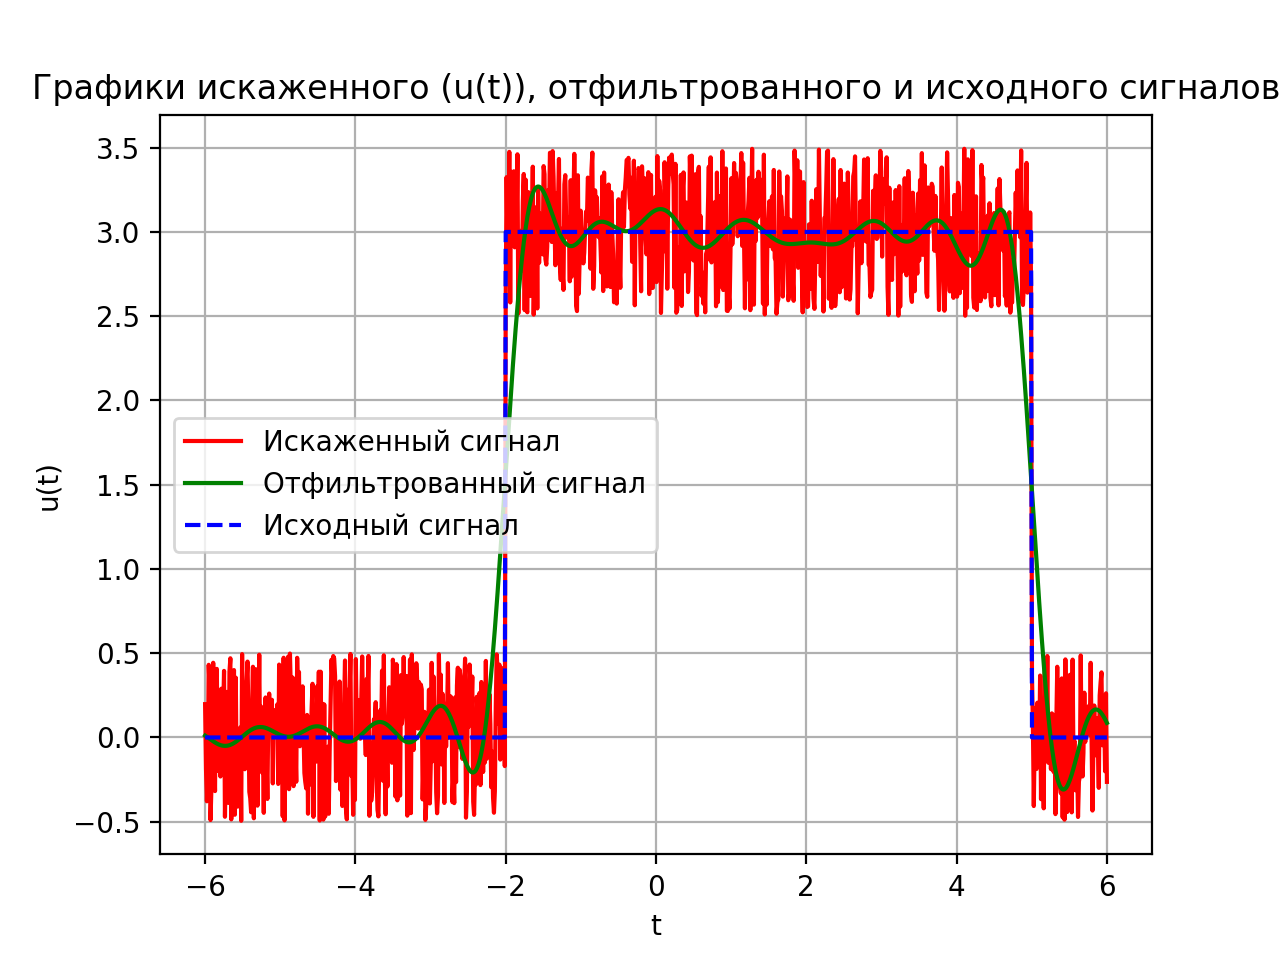
\includegraphics[scale=0.85]{media/1 task/high_freq/Cleaned_1_-1,1981981981981982.png}
    \caption{Графики  $u(t)$, отфильтрованного и исходного сигналов при $b=1$ и $\nu_0=1.2$ Гц} 
    \label{fig:cleaned_1_12}
\end{figure}

\begin{figure}[ht!]
    \centering
    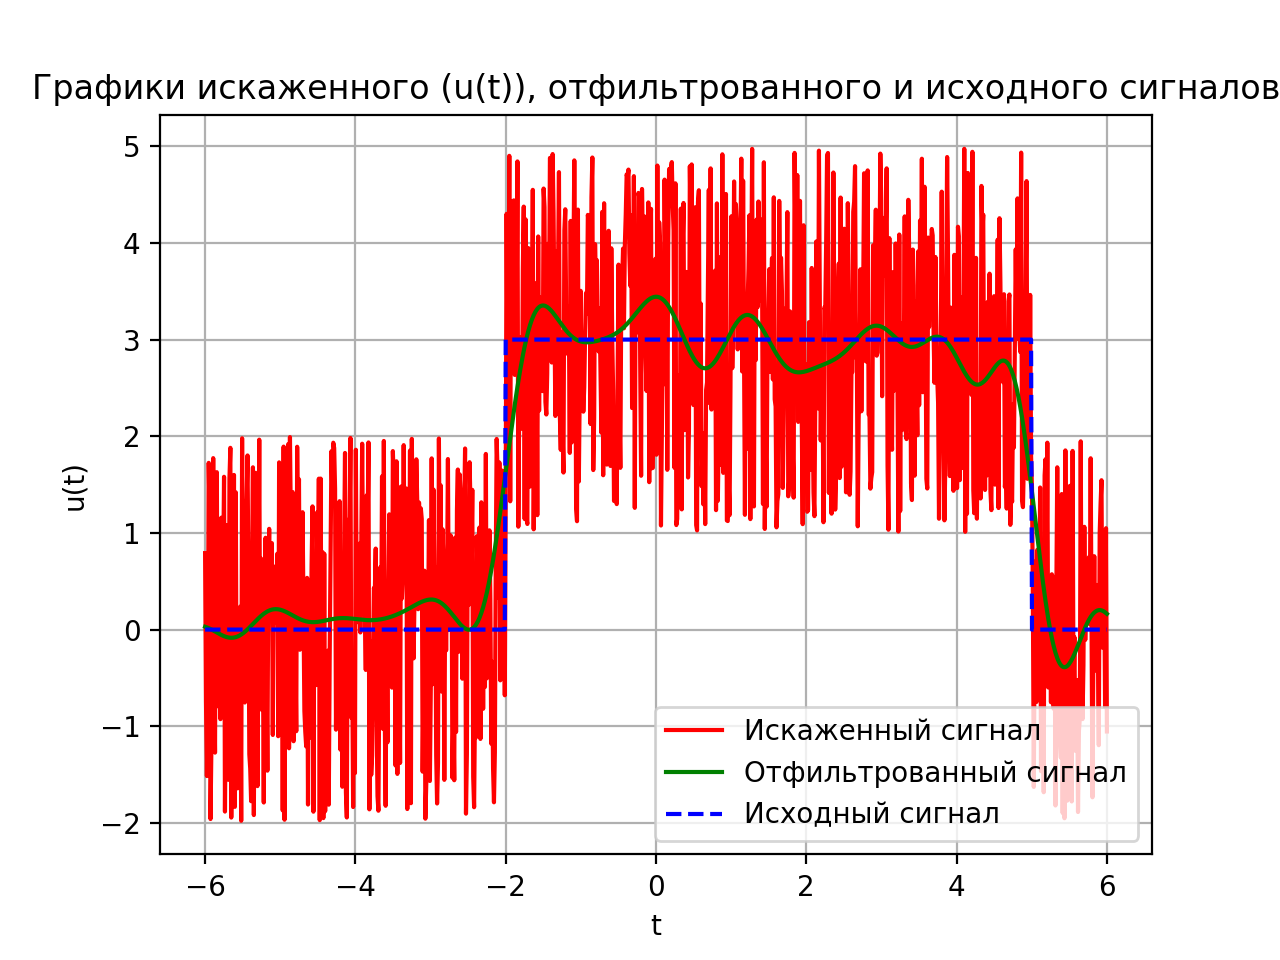
\includegraphics[scale=0.85]{media/1 task/high_freq/Cleaned_4_-1,1981981981981982.png}
    \caption{Графики  $u(t)$, отфильтрованного и исходного сигналов при $b=4$ и $\nu_0=1.2$ Гц}
    \label{fig:cleaned_4_12}
\end{figure}

Обратим внимание на модули Фурье-образов при значениях $0.25, 1, 4$ параметра $b$ (рисунки \ref{fig:four_025_12}, \ref{fig:four_1_12} и \ref{fig:four_4_12} соответственно). Стоит отметить, что при увеличении значения графики модуля Фурье-образа становятся более хаотичным при высоких частотах. Это свидетельствует о том, что увеличивается влияние высокочастотного шума на сигнал $u(t)$. Далее перейдём к графикам отфильтрованного сигнала (рисунки \ref{fig:cleaned_025_12}, \ref{fig:cleaned_1_12}, \ref{fig:cleaned_4_12}). При увеличении параметра уменьшается приближение отфильтрованного сигнала к исходному по норме, что является признаком большего влияния высокочастотного шума на сигнал. Однако это приводит к тому, что при большем значении $b$ отфильтрованный сигнал имеет меньше колебаний, так как высокочастотные компоненты Фурье-образа в большей степени вызваны искажением сигнала, а не природой исходной функции $g(t)$. 

\clearpage
\subsection{Специфические частоты}

Теперь мы будем оставлять значение лишь определённого диапазона частот при фильтрации. Это означает, что мы будем отбрасывать частоты таким образом, чтобы график модуля образа Фурье отфильтрованного сигнала как можно точнее совпадал с аналогичным графиком исходного сигнала $g(t)$. Для того, чтобы проанализировать влияние параметров на фильтрацию сигнала, мы для начала зафиксируем диапазон определённых частот, а затем рассмотрим влияние частот среза. В этом пункте параметры $c$ и $d$ будут ненулевыми.

\subsubsection{Рассматриваем зашумленные сигналы при $b=0$}\label{b_0}

Начнём наши ислледования при $b=0$. Строим графики аналогично пункту выше и анализируем их:

\begin{figure}[ht!]
    \centering
    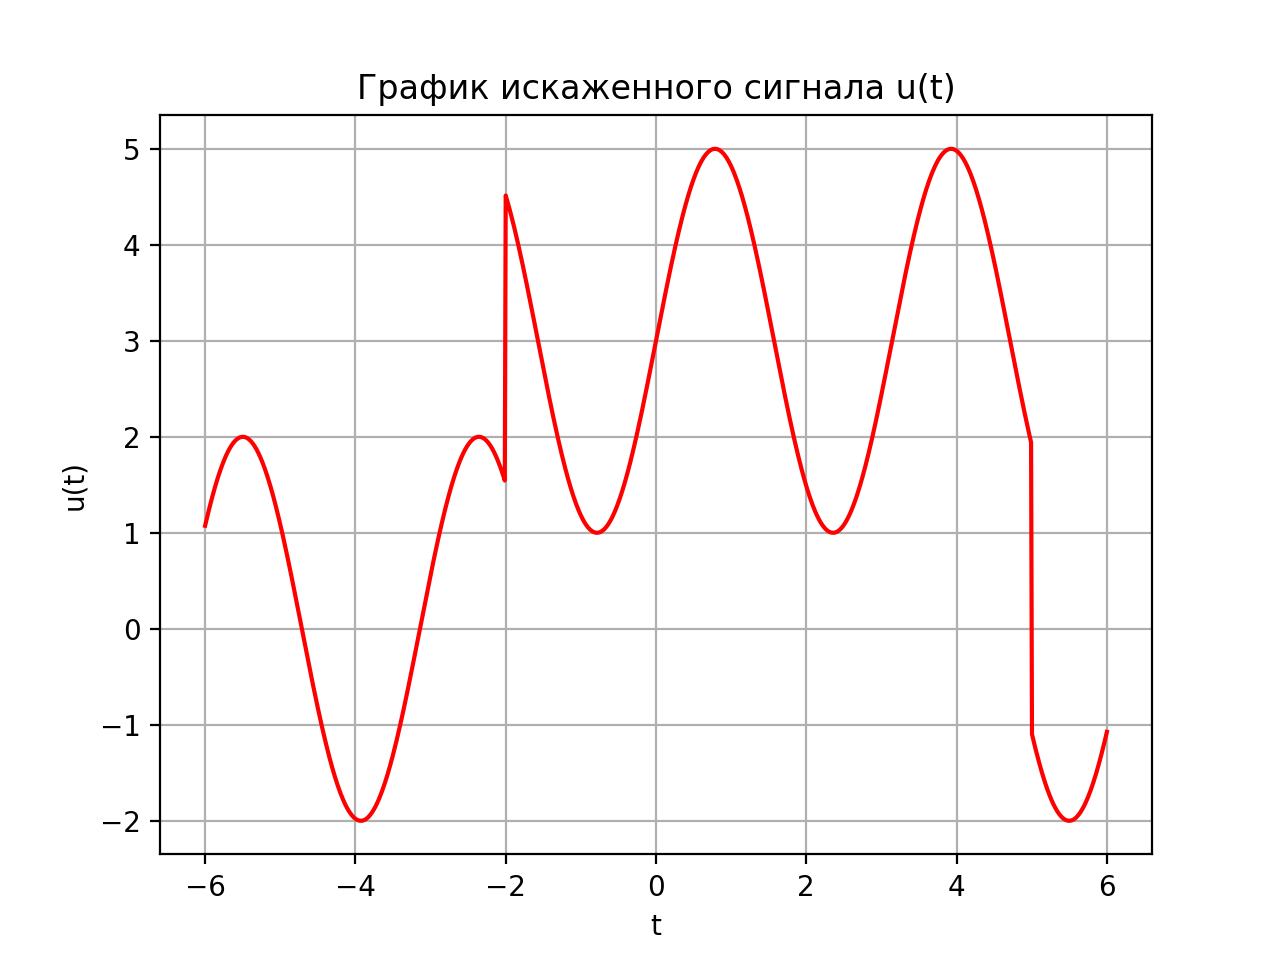
\includegraphics[scale=0.75]{media/1 task/specific_freq/Noisy_0_2_2.png}
    \caption{График функции $u(t)$ при $b=0$,  $c=2$,  $d=2$}
    \label{fig:noisy_0_2_2}
\end{figure}

\clearpage

\begin{figure}[ht!]
    \centering
    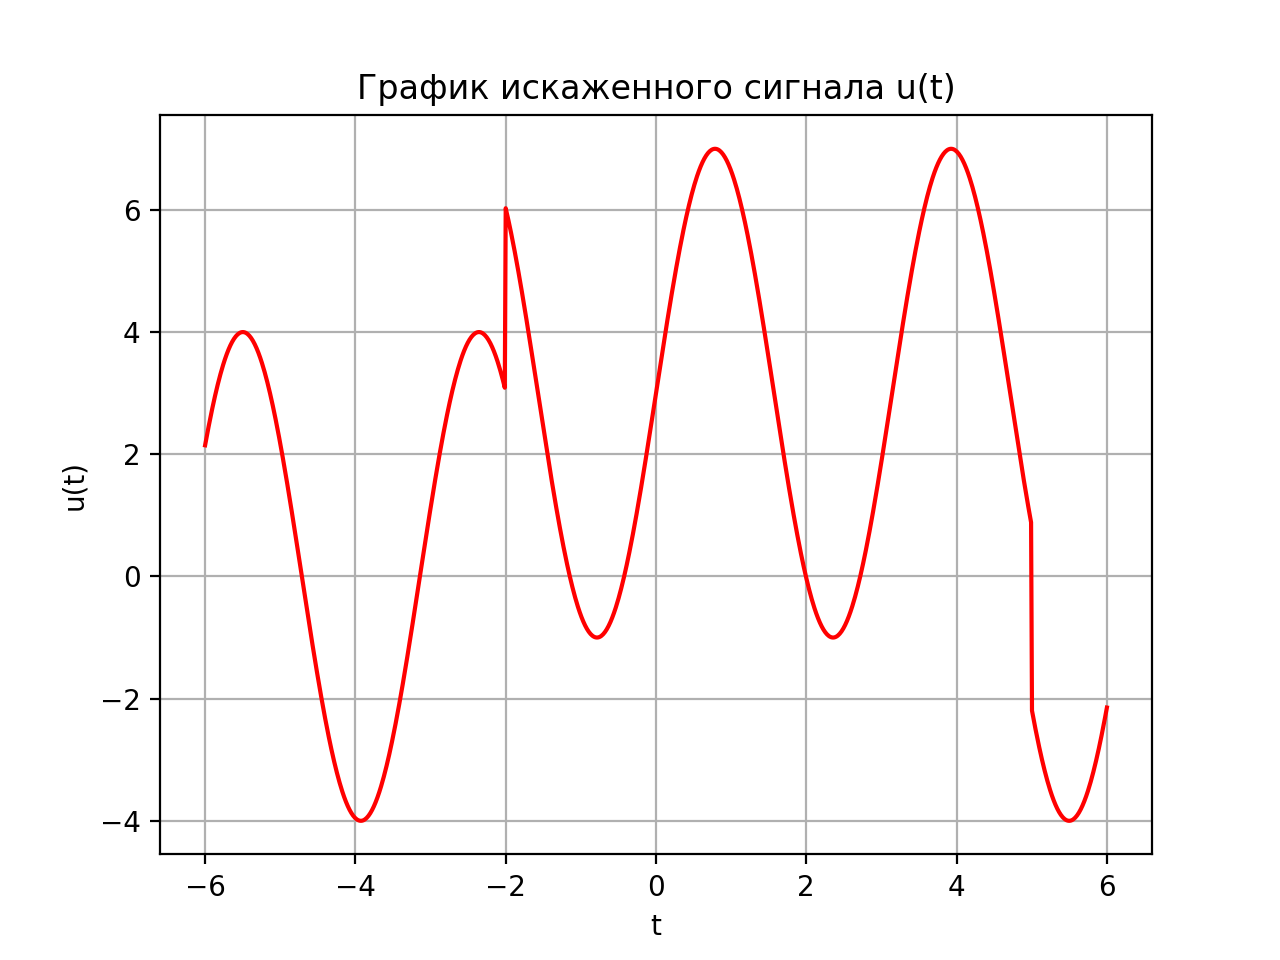
\includegraphics[scale=0.75]{media/1 task/specific_freq/Noisy_0_4_2.png}
    \caption{График функции $u(t)$ при $b=0$,  $c=4$,  $d=2$}
    \label{fig:noisy_0_4_2}
\end{figure}

\begin{figure}[ht!]
    \centering
    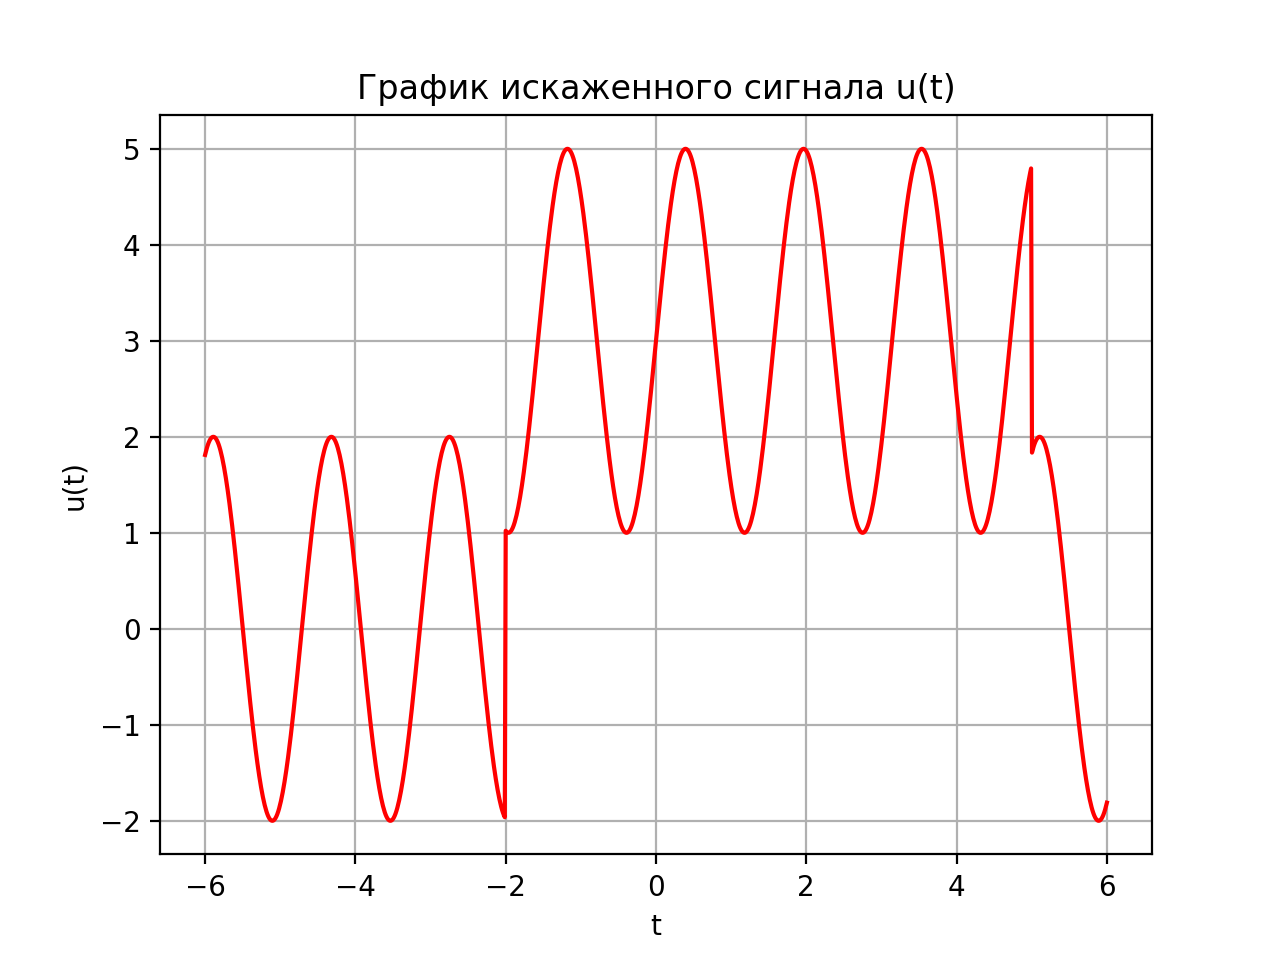
\includegraphics[scale=0.75]{media/1 task/specific_freq/Noisy_0_2_4.png}
    \caption{График функции $u(t)$ при $b=0$,  $c=2$,  $d=4$}
    \label{fig:noisy_0_2_4}
\end{figure}

На основе графиков можно сделать вывод, что параметр $c$ влияет на амплитуду зашумленного сигнала, параметр $d$ --- частоту сигнала. Теперь оценим влияние этих параметров на фильтрацию при исключении частот $\nu_0\in[0.22, 1.0] \cup [2.7, 2.99]$ Гц:


\begin{figure}[ht!]
    \centering
    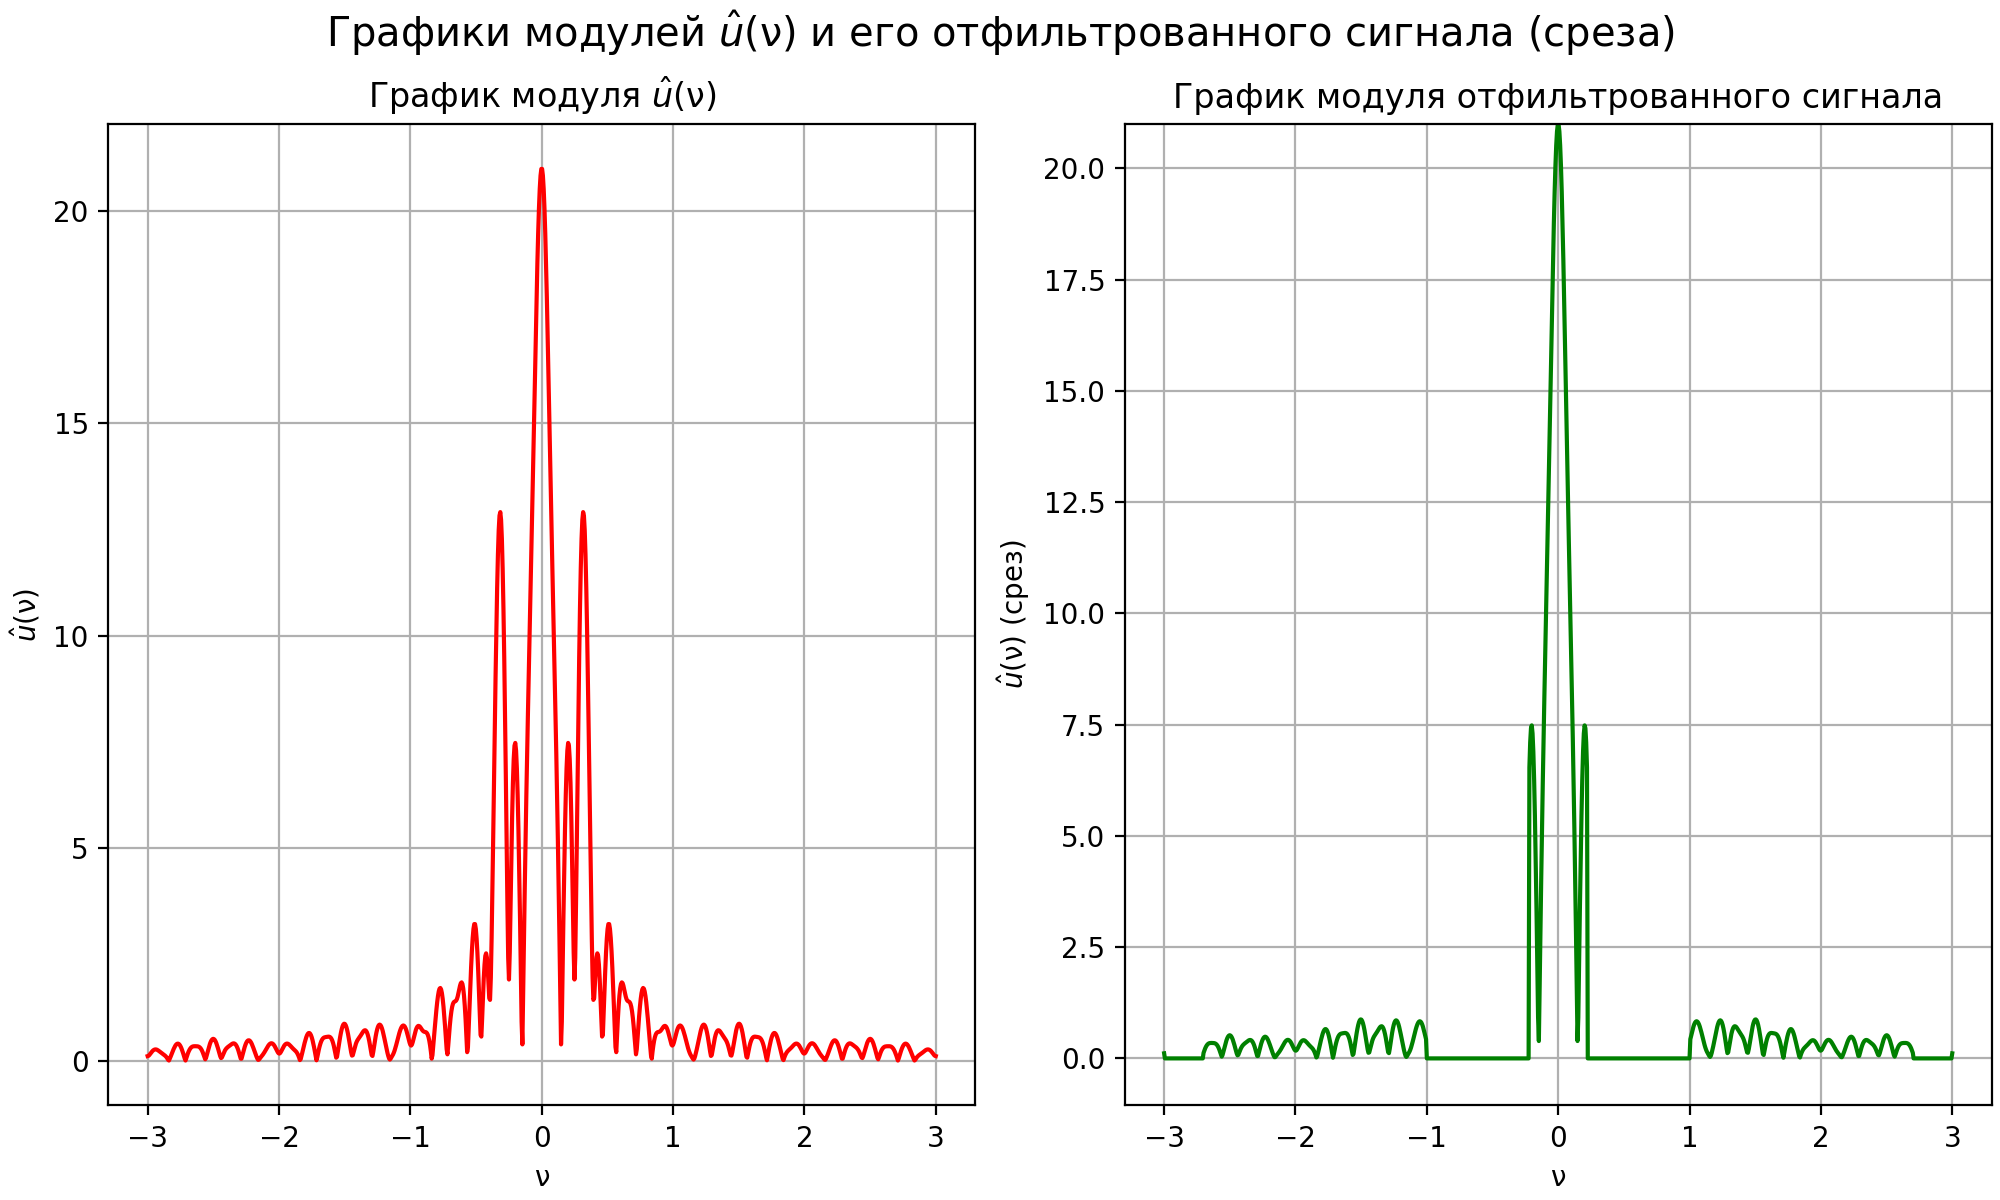
\includegraphics[scale=0.55]{media/1 task/specific_freq/Fourier_Image_0_2_2_-1,0_-0,22_-2,99_-2,7.png}
    \caption{Графики модулей Фурье-образа $u(t)$ и отфильтрованного сигнала при $b=0$,  $c=2$,  $d=2$}
    \label{fig:four_0_2_2}
\end{figure}

\begin{figure}[ht!]
    \centering
    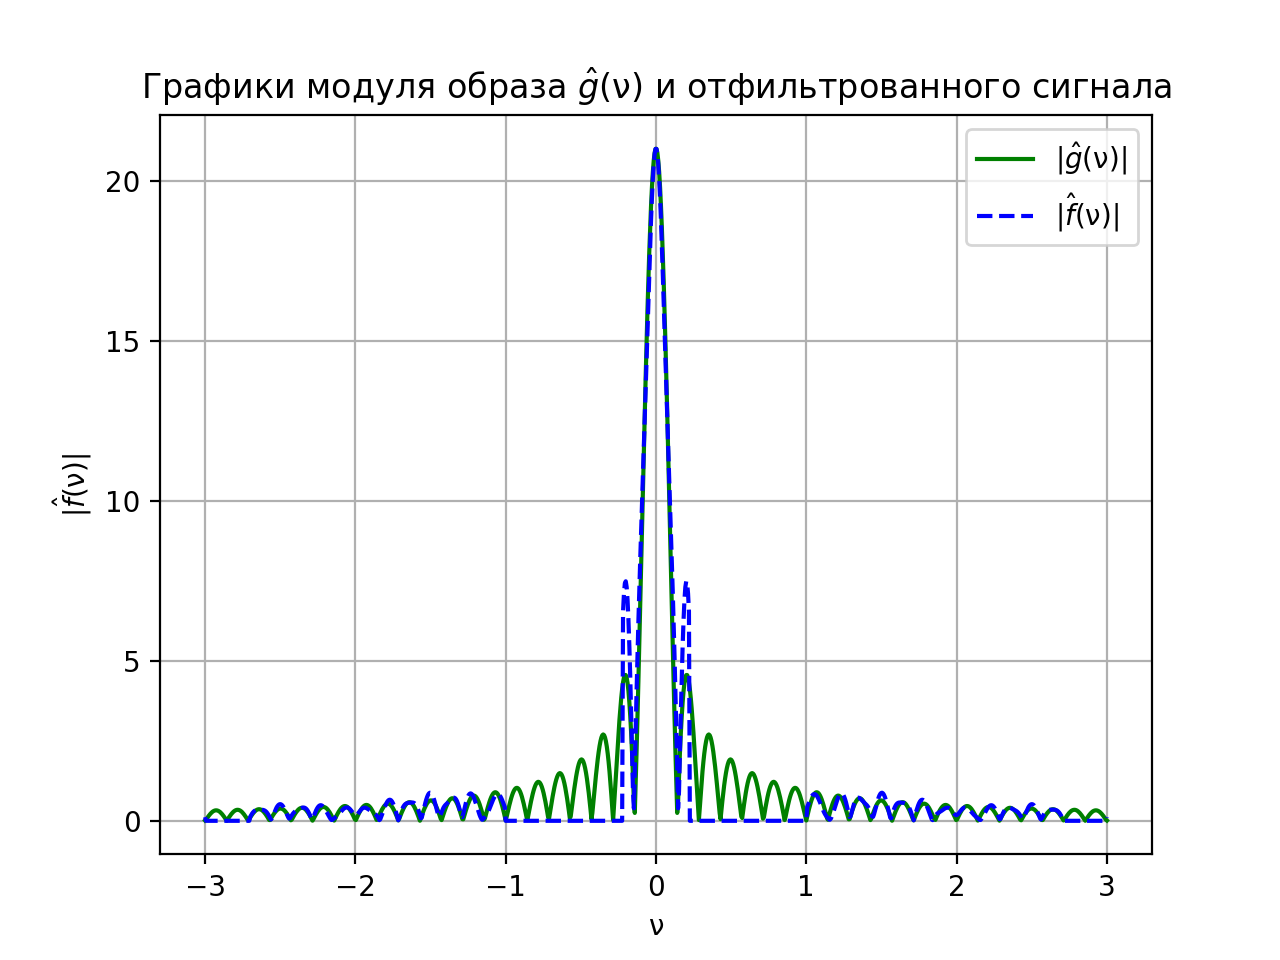
\includegraphics[scale=0.55]{media/1 task/specific_freq/Fourier_Image_Comparison_0_2_2_-1,0_-0,22_-2,99_-2,7.png}
    \caption{Сравнительные графики модулей Фурье-образа $g(t)$ и отфильтрованного сигнала при $b=0$,  $c=2$,  $d=2$}
    \label{fig:fourc_0_2_2}
\end{figure}

\begin{figure}[ht!]
    \centering
    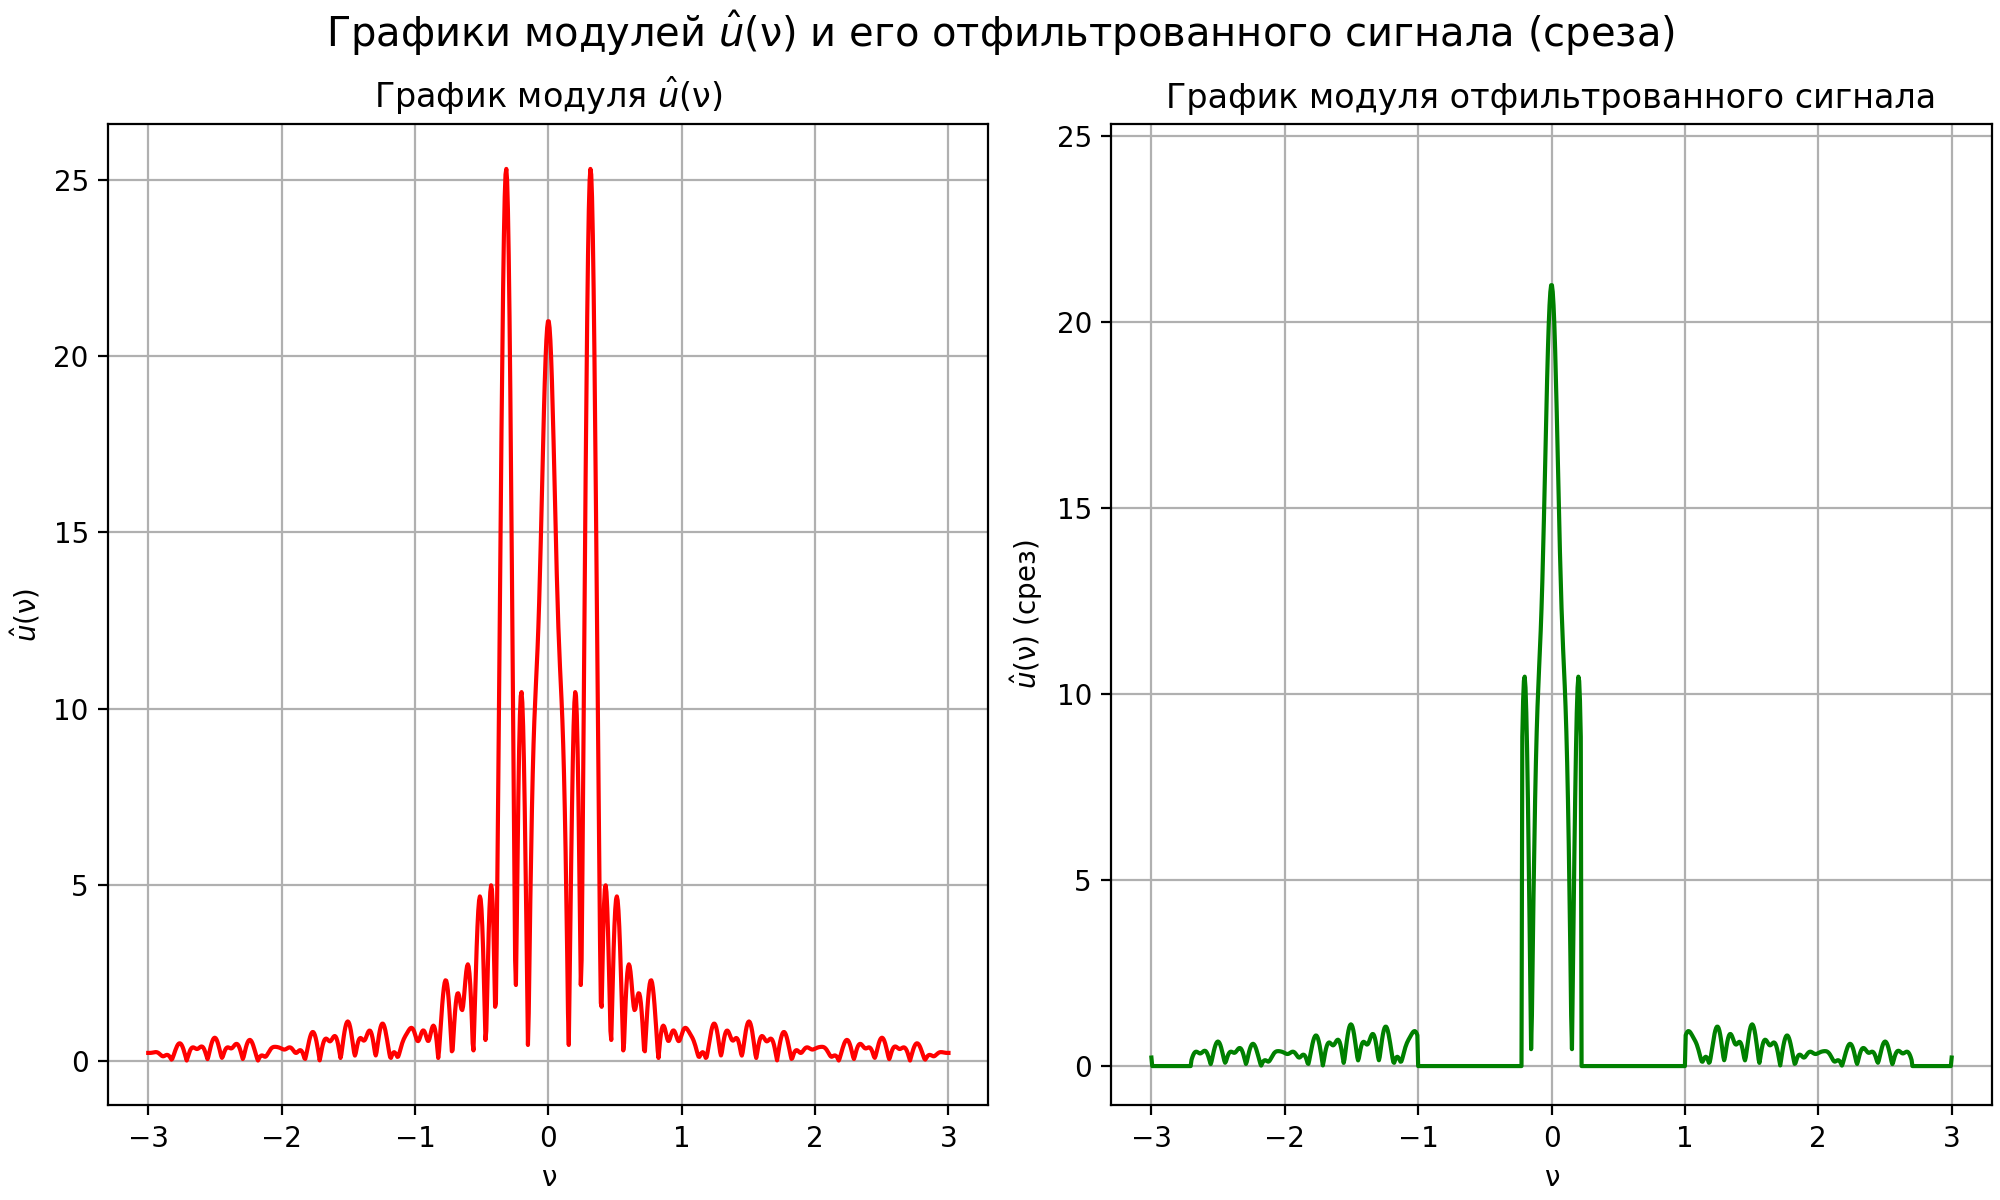
\includegraphics[scale=0.55]{media/1 task/specific_freq/Fourier_Image_0_4_2_-1,0_-0,22_-2,99_-2,7.png}
    \caption{Графики модулей Фурье-образа $u(t)$ и отфильтрованного сигнала при $b=0$,  $c=4$,  $d=2$}
    \label{fig:four_0_4_2}
\end{figure}

\begin{figure}[ht!]
    \centering
    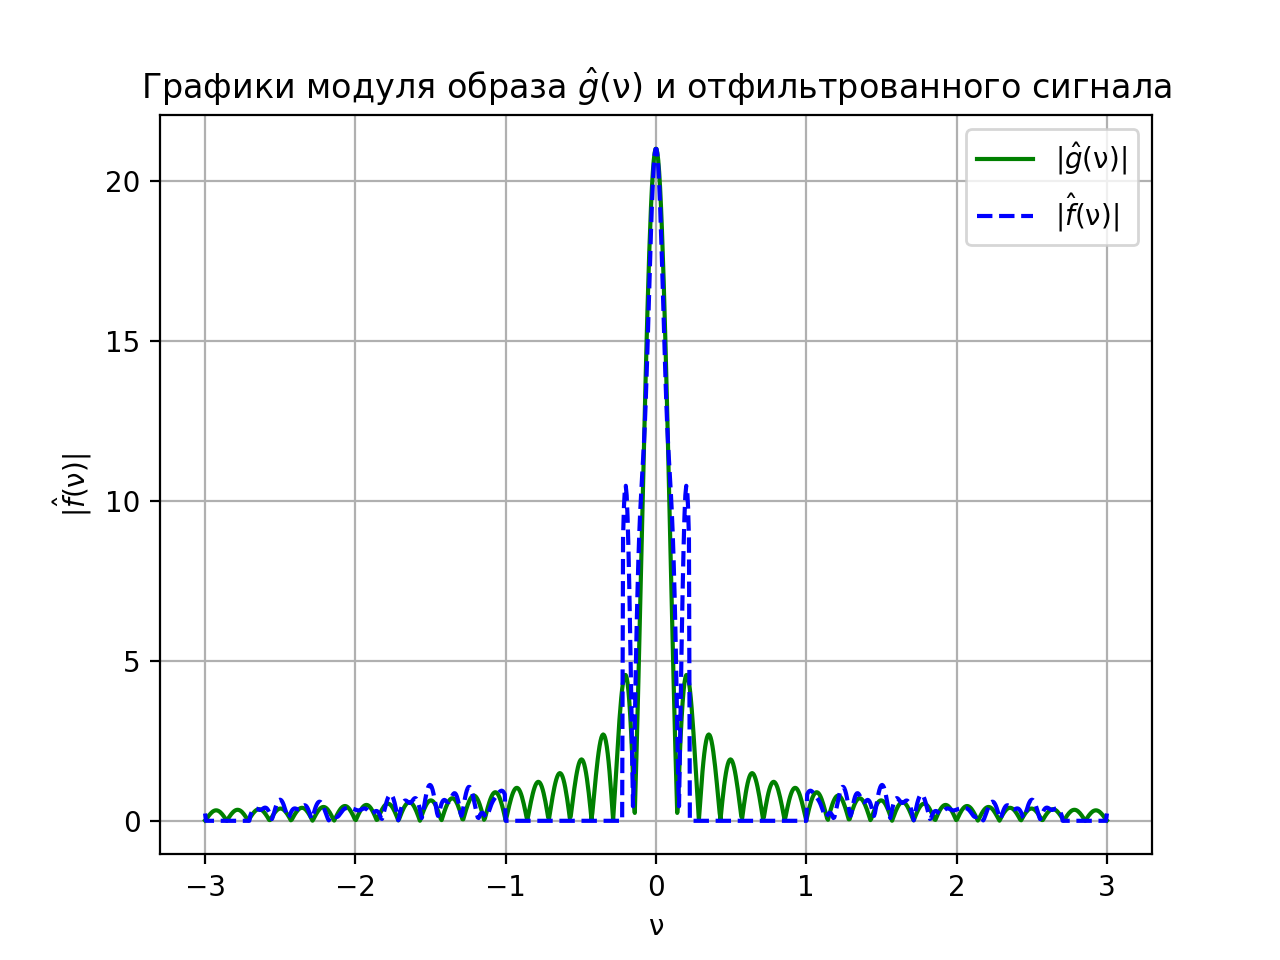
\includegraphics[scale=0.55]{media/1 task/specific_freq/Fourier_Image_Comparison_0_4_2_-1,0_-0,22_-2,99_-2,7.png}
    \caption{Сравнительные графики модулей Фурье-образа $g(t)$ и отфильтрованного сигнала при $b=0$,  $c=4$,  $d=2$}
    \label{fig:fourc_0_4_2}
\end{figure}

\clearpage

\begin{figure}[ht!]
    \centering
    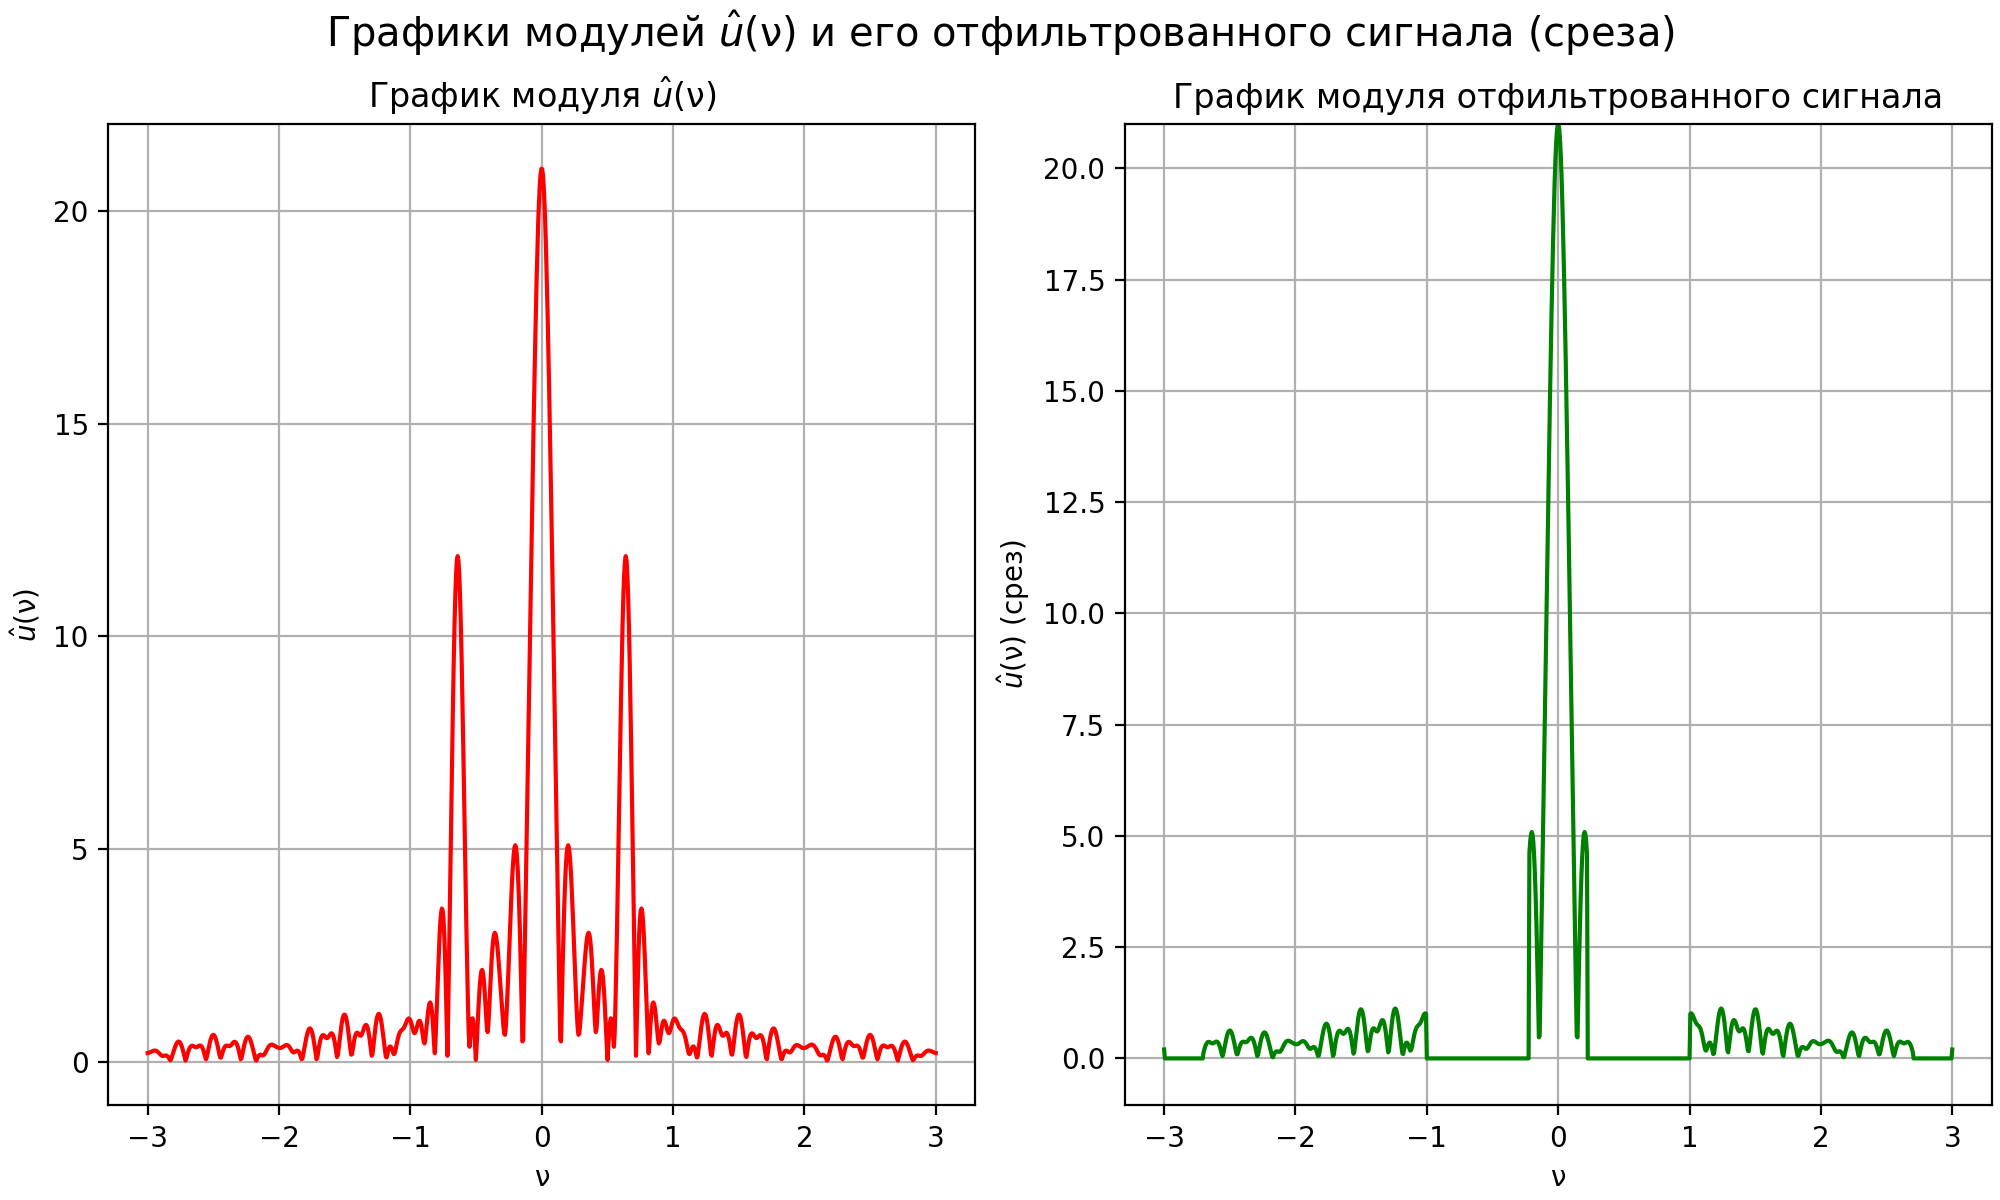
\includegraphics[scale=0.55]{media/1 task/specific_freq/Fourier_Image_0_2_4_-1,0_-0,22_-2,99_-2,7.png}
    \caption{Графики модулей Фурье-образа $f(t)$ и отфильтрованного сигнала при $b=0$,  $c=2$,  $d=4$}
    \label{fig:four_0_2_4}
\end{figure}

\begin{figure}[ht!]
    \centering
    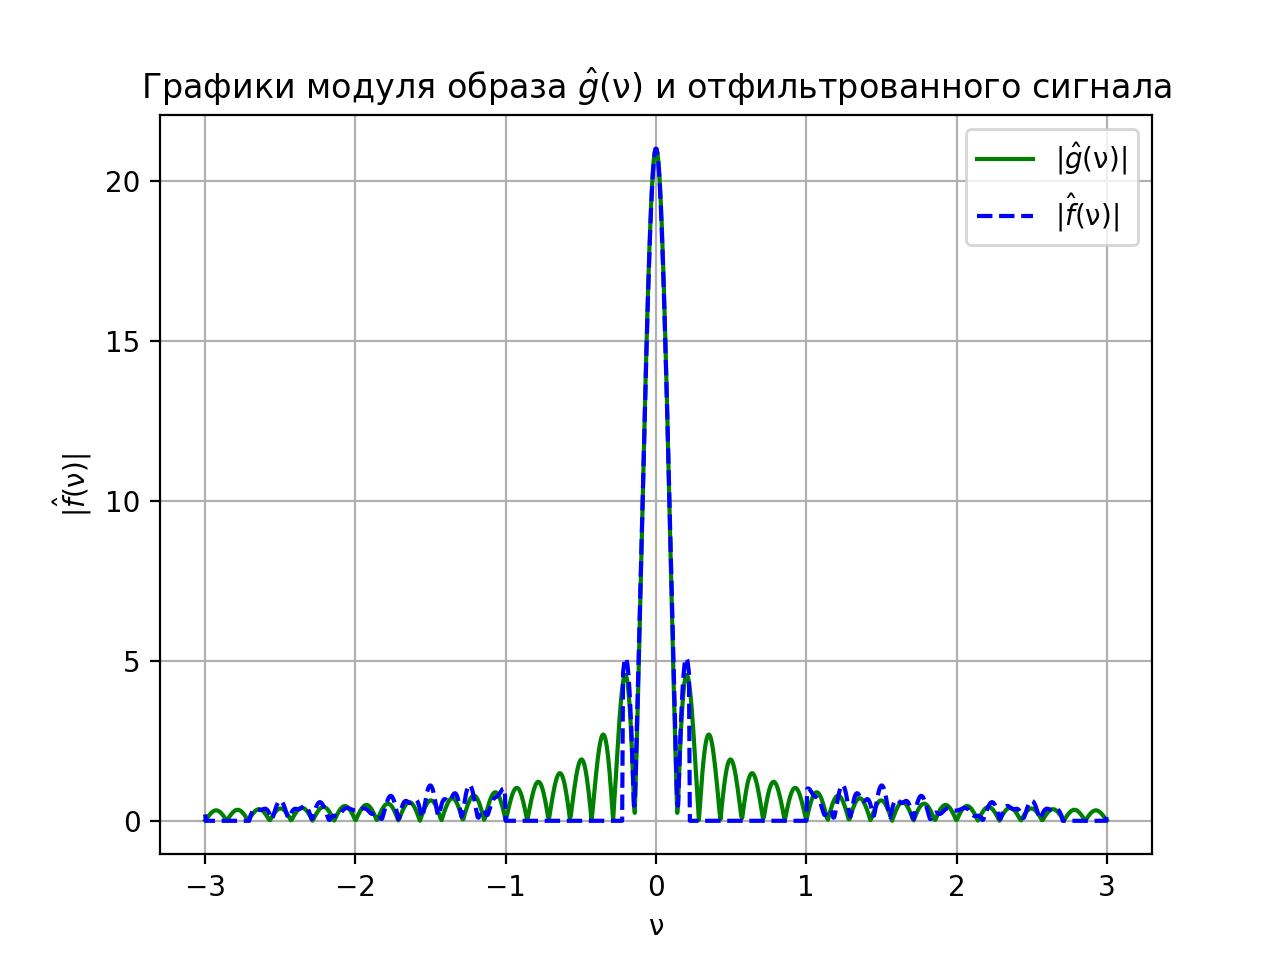
\includegraphics[scale=0.55]{media/1 task/specific_freq/Fourier_Image_Comparison_0_2_4_-1,0_-0,22_-2,99_-2,7.png}
    \caption{Сравнительные графики модулей Фурье-образа $g(t)$ и отфильтрованного сигнала при  $b=0$,  $c=2$,  $d=4$}
    \label{fig:fourc_0_2_4}
\end{figure}

Скачки на графике модуля Фурье-образа обуславливаются доминирующими частотами. При увеличении параметра $d$ увеличивается частота зашумленного сигнала, на Фурье-образе это отражается смещением пиков и шумов в сторону более высоких частот. Параметр $c$ влияет на амплитуду сигнала, поэтому при увеличении параметра $c$ увеличиваются значения модуля Фурье-образа практически на всём диапазоне частот, особенно в окрестности основной частоты сигнала. Поэтому для фильтрации сигнала мы должны исключить данную окрестность и затем попробовать снизить колебания отфильтрованного графика обнулением высоких частот: 

\begin{figure}[ht!]
    \centering
    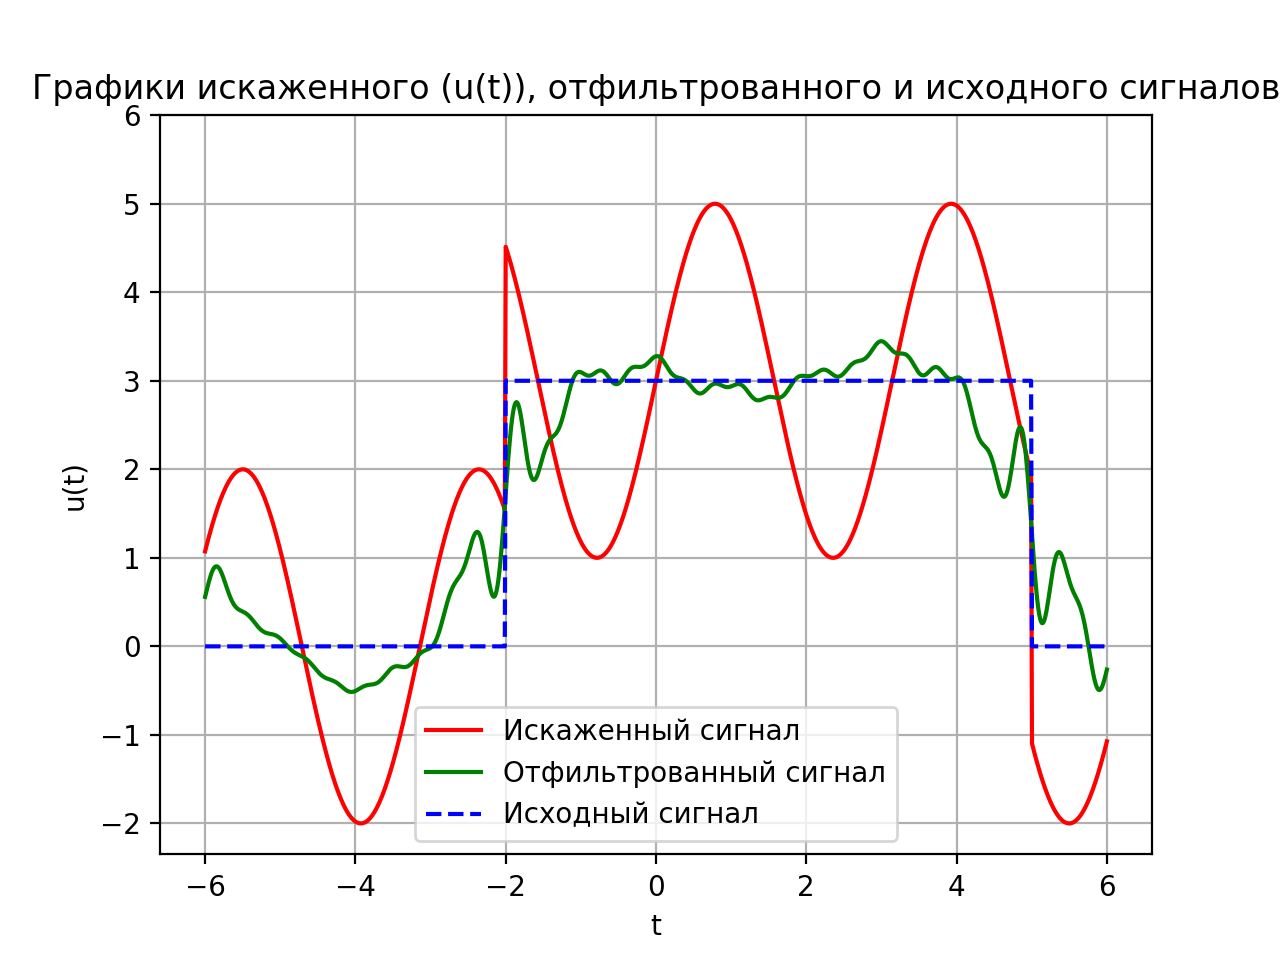
\includegraphics[scale=0.75]{media/1 task/specific_freq/Cleaned_0_2_2_-1,0_-0,22_-2,99_-2,7.png}
    \caption{Графики  $u(t)$, отфильтрованного и исходного сигналов при $b=0$,  $c=2$,  $d=2$}
    \label{fig:cleaned_0_2_2}
\end{figure}

\begin{figure}[ht!]
    \centering
    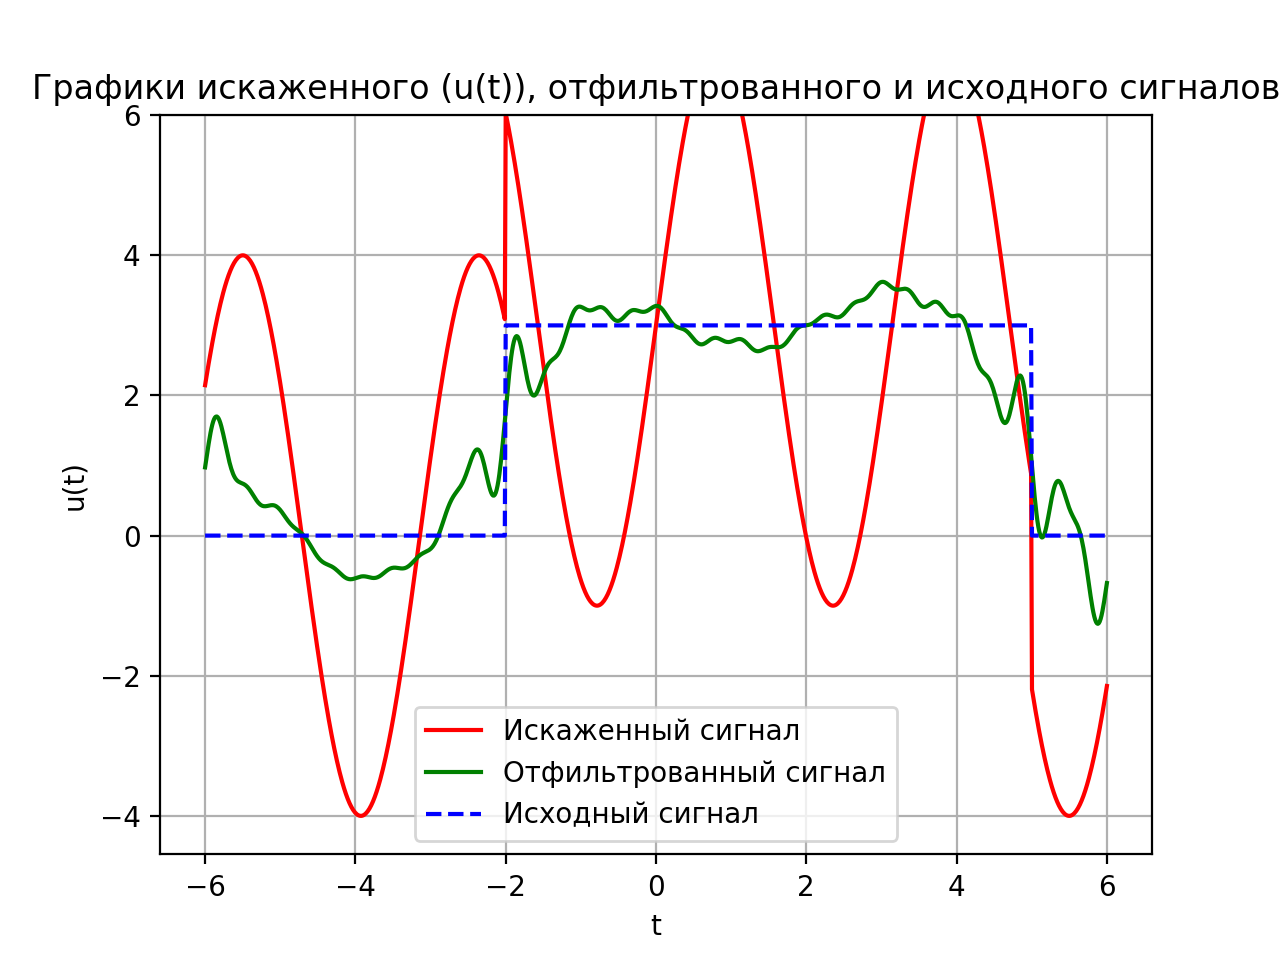
\includegraphics[scale=0.75]{media/1 task/specific_freq/Cleaned_0_4_2_-1,0_-0,22_-2,99_-2,7.png}
    \caption{Графики  $u(t)$, отфильтрованного и исходного сигналов при $b=0$,  $c=4$,  $d=2$}
    \label{fig:cleaned_0_4_2}
\end{figure}

\clearpage

\begin{figure}[ht!]
    \centering
    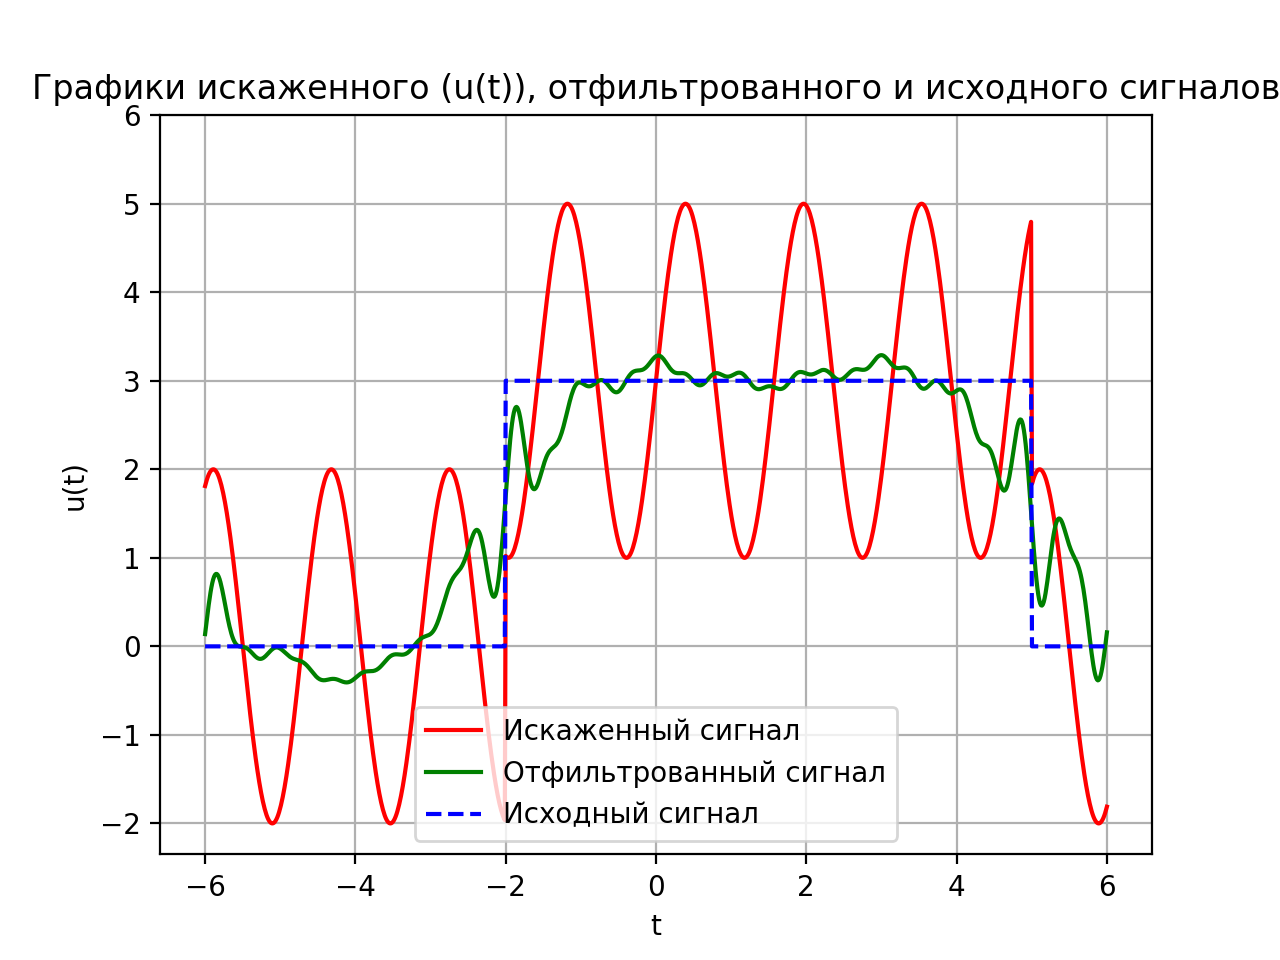
\includegraphics[scale=0.75]{media/1 task/specific_freq/Cleaned_0_2_4_-1,0_-0,22_-2,99_-2,7.png}
    \caption{Графики  $u(t)$, отфильтрованного и исходного сигналов при $b=0$,  $c=2$,  $d=4$}
    \label{fig:cleaned_0_2_4}
\end{figure}

Сравнение графиков подтверждают ранее сделанные выводы. Увеличение параметра $c$ приводит к увеличению значений пиков отфильтрованного сигнала. При увеличении параметра $b$ увеличиваются колебания на <<площадках>> сигнала из-за увеличения частоты зашумленного сигнала. 

\clearpage

\subsubsection{Влияние параметра $b$}\label{b_ex}

Теперь рассмотрим влияние параметра $b$ на фильтрацию. Зафиксируем параметры $c=4, d=2$ и частоты  $\nu_0 \in [0.22, 0.6] \cup [1.6, 2.99]$

\begin{figure}[ht!]
    \centering
    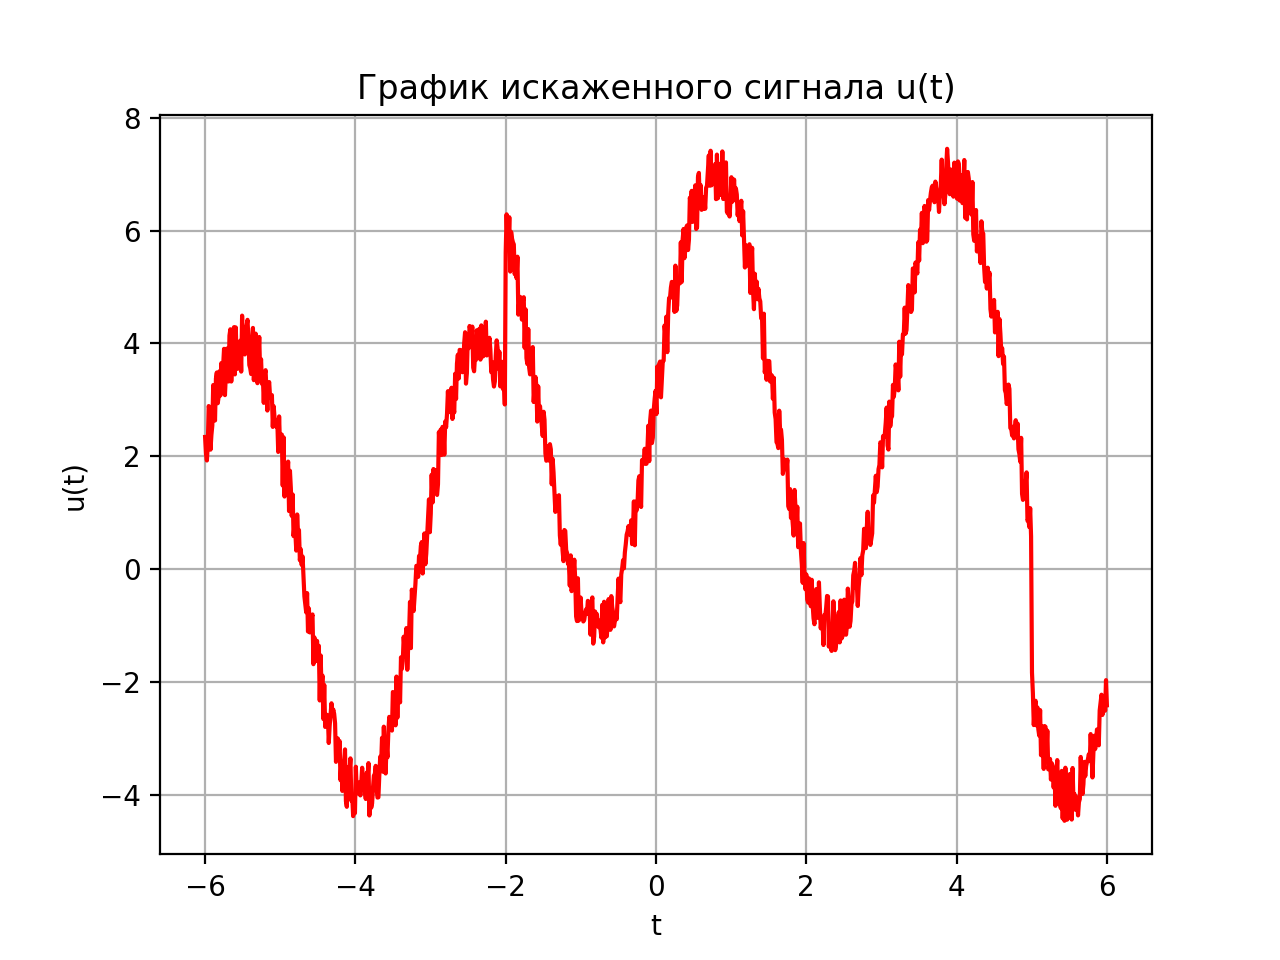
\includegraphics[scale=0.75]{media/1 task/specific_freq/Noisy_1_4_2.png}
    \caption{График функции $u(t)$ при $b=1$,  $c=4$,  $d=2$}
    \label{fig:noisy_1_4_2}
\end{figure}

\begin{figure}[ht!]
    \centering
    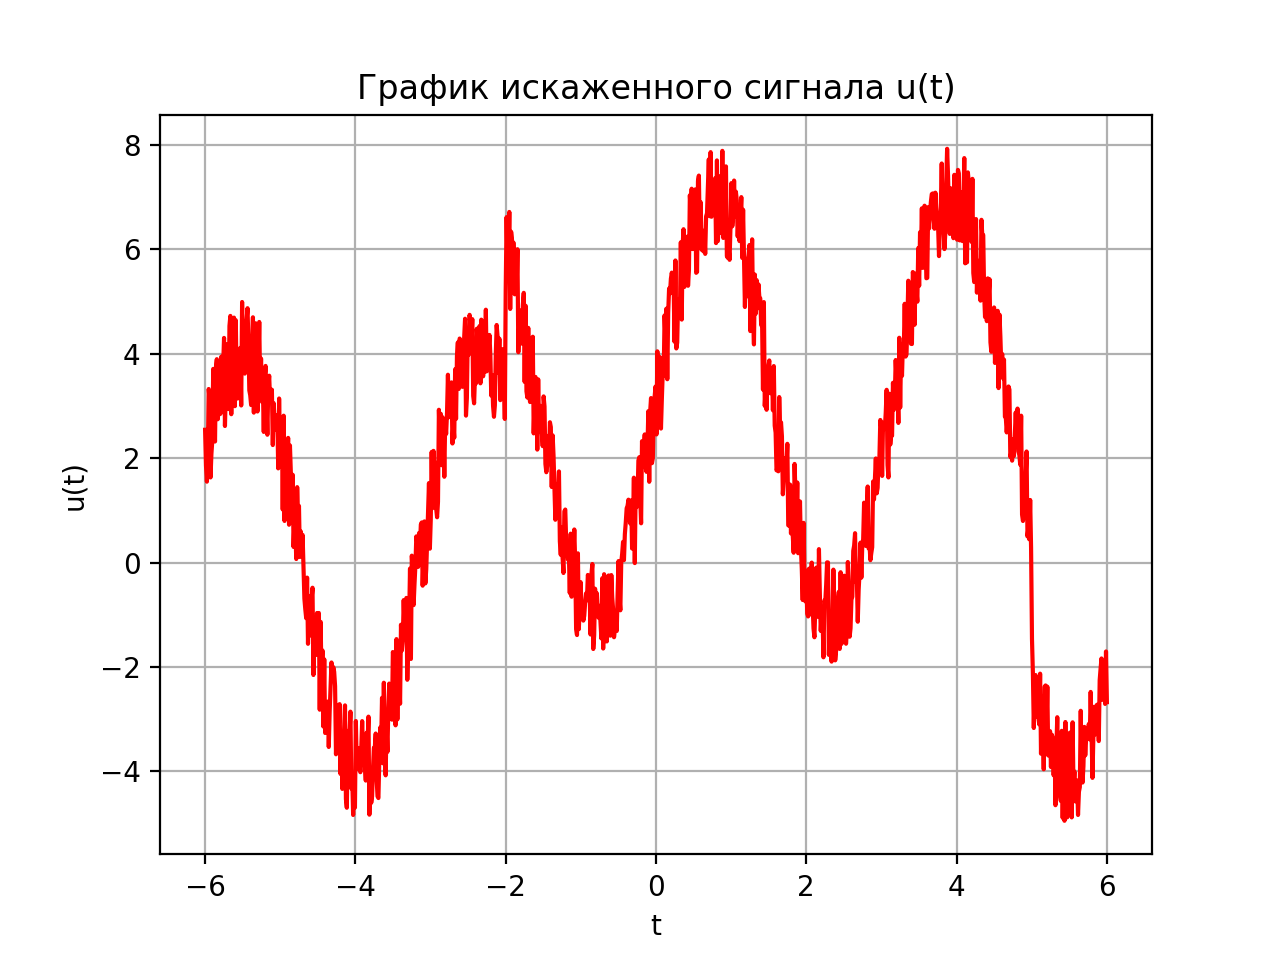
\includegraphics[scale=0.75]{media/1 task/specific_freq/Noisy_2_4_2.png}
    \caption{График функции $u(t)$ при $b=2$,  $c=4$,  $d=2$}
    \label{fig:noisy_2_4_2}
\end{figure}

\clearpage

\begin{figure}[ht!]
    \centering
    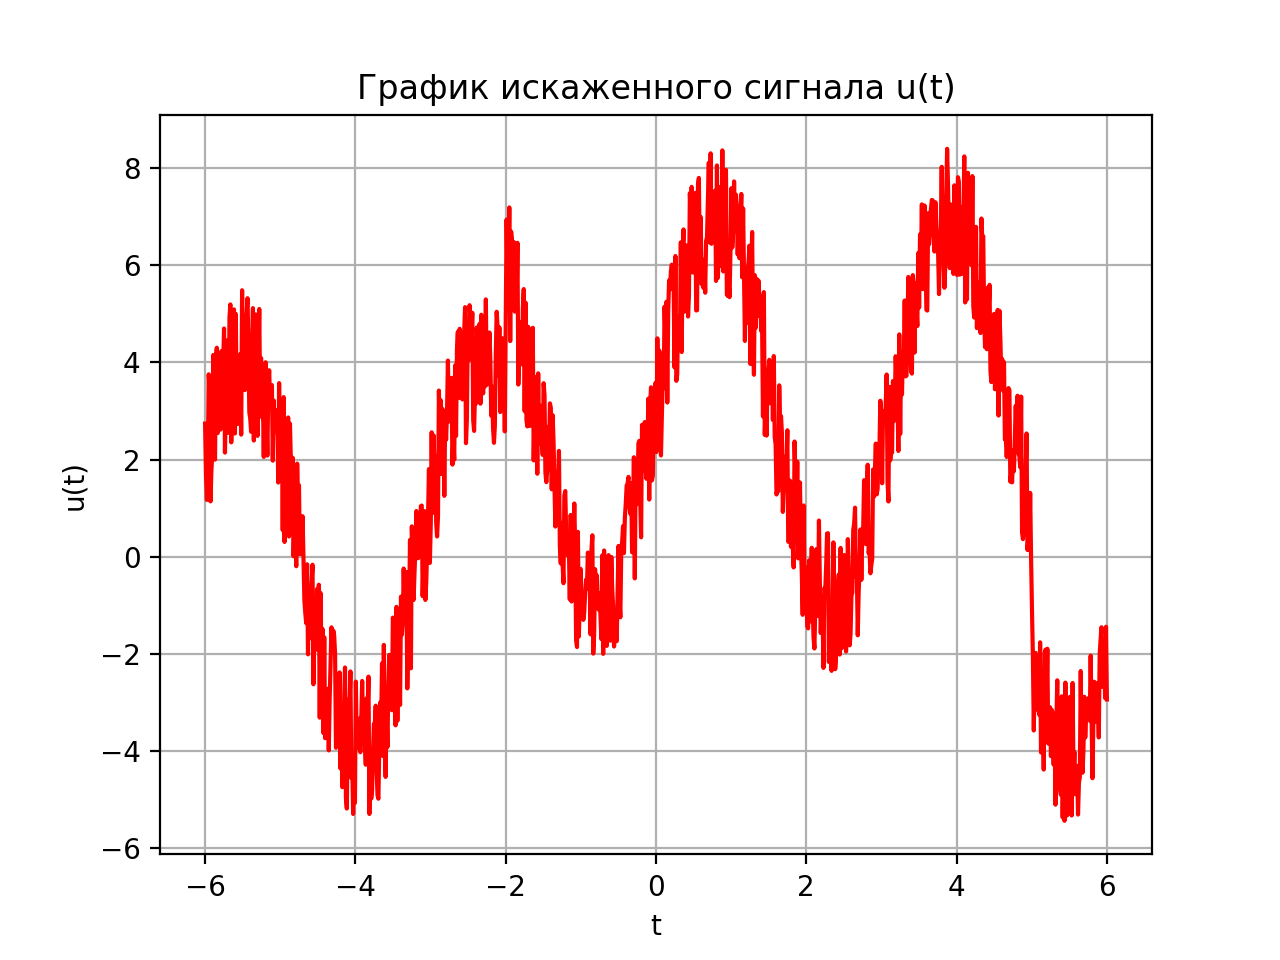
\includegraphics[scale=0.75]{media/1 task/specific_freq/Noisy_3_4_2.png}
    \caption{График функции $u(t)$ при $b=3$,  $c=4$,  $d=2$}
    \label{fig:noisy_3_4_2}
\end{figure}

Графики подтверждают вывод, сделанный в пункте \ref{high_freq}, о влиянии параметра $b$ на хаотический шум в зашумленном сигнале. А мы идём дальше к Фурье-образам!

\clearpage

\begin{figure}[ht!]
    \centering
    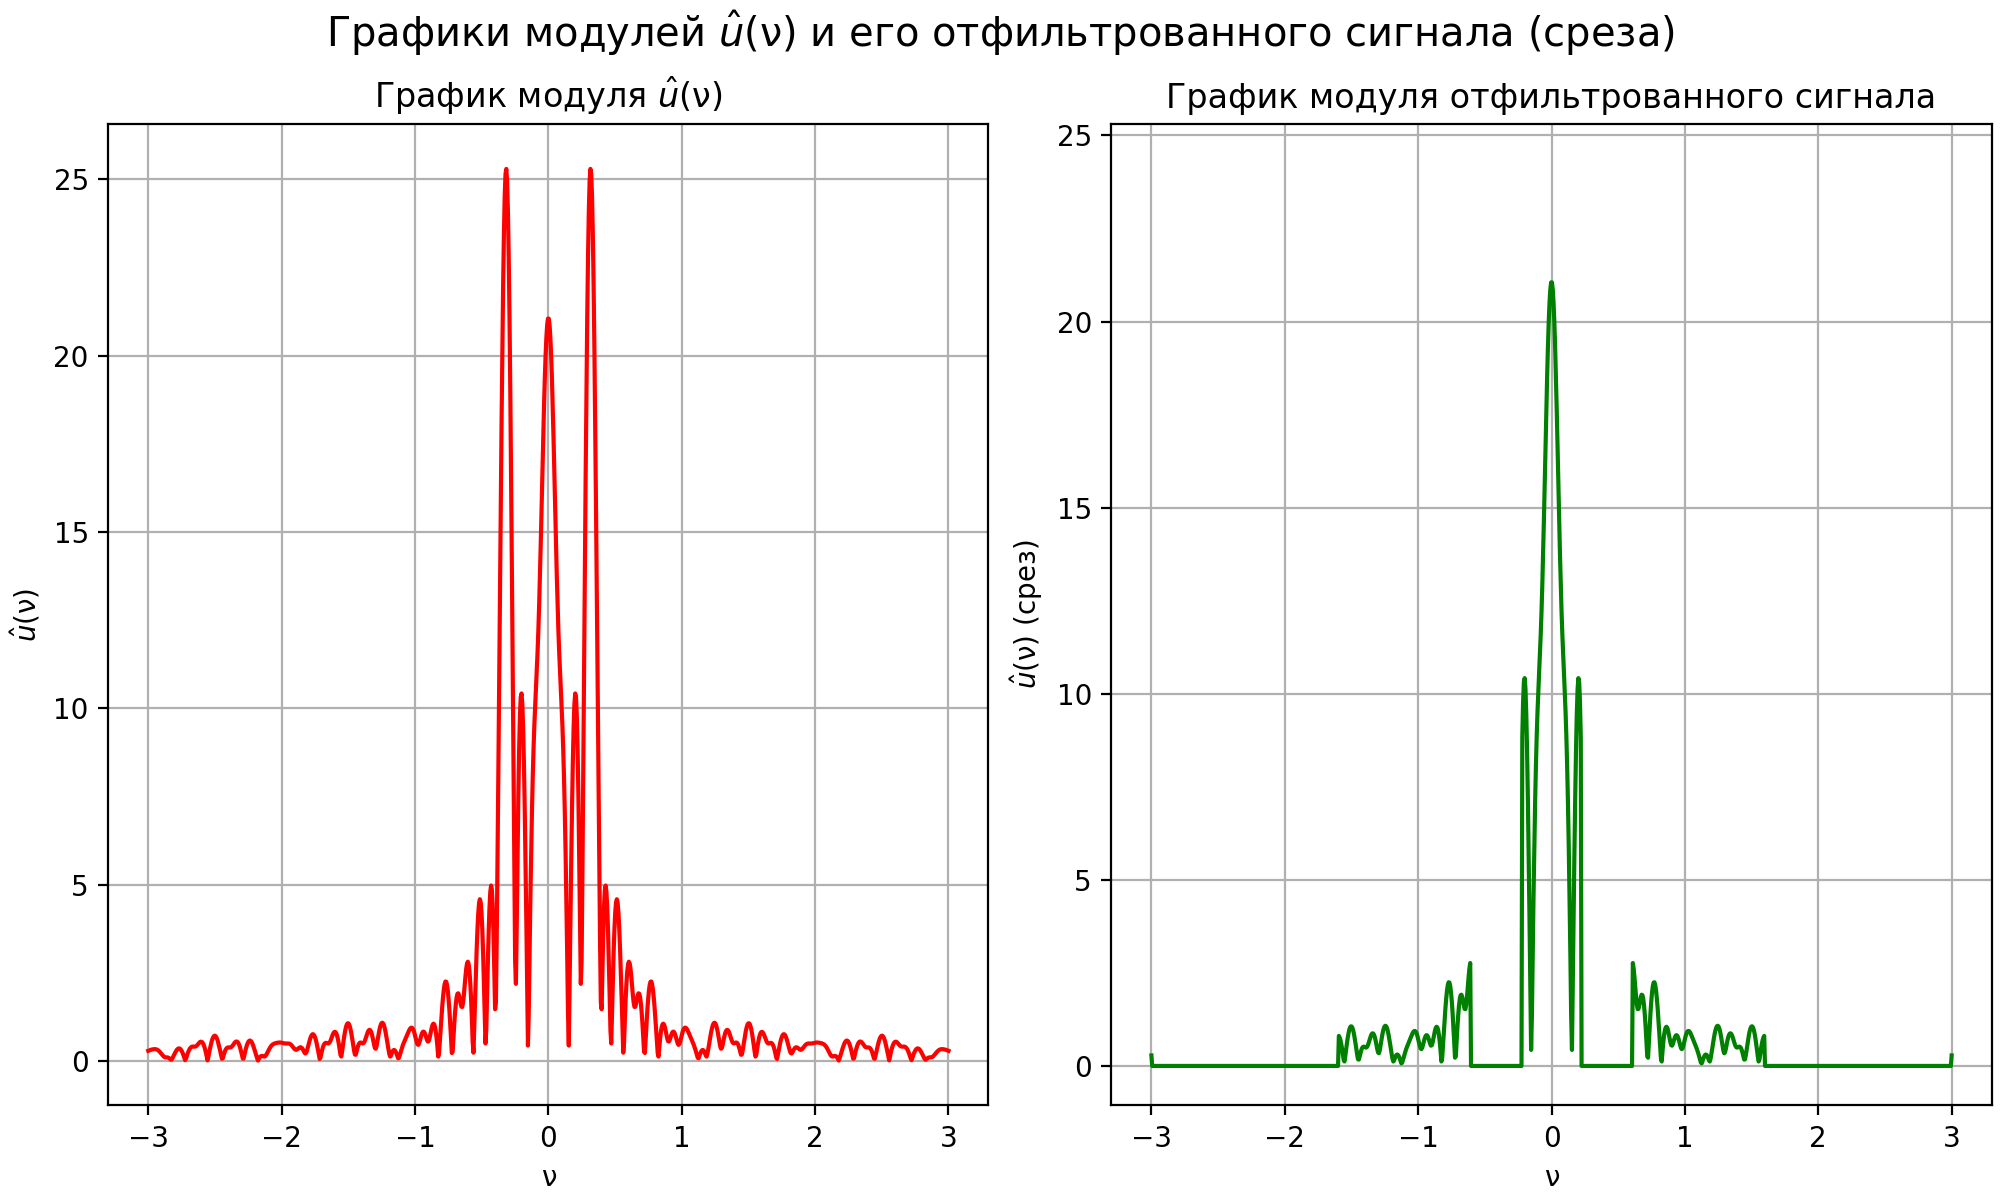
\includegraphics[scale=0.55]{media/1 task/specific_freq/Fourier_Image_1_4_2_-0,6_-0,22_-2,99_-1,6.png}
    \caption{Графики модулей Фурье-образа $u(t)$ и отфильтрованного сигнала при $b=1$,  $c=4$,  $d=2$}
    \label{fig:four_1_4_2}
\end{figure}


\begin{figure}[ht!]
    \centering
    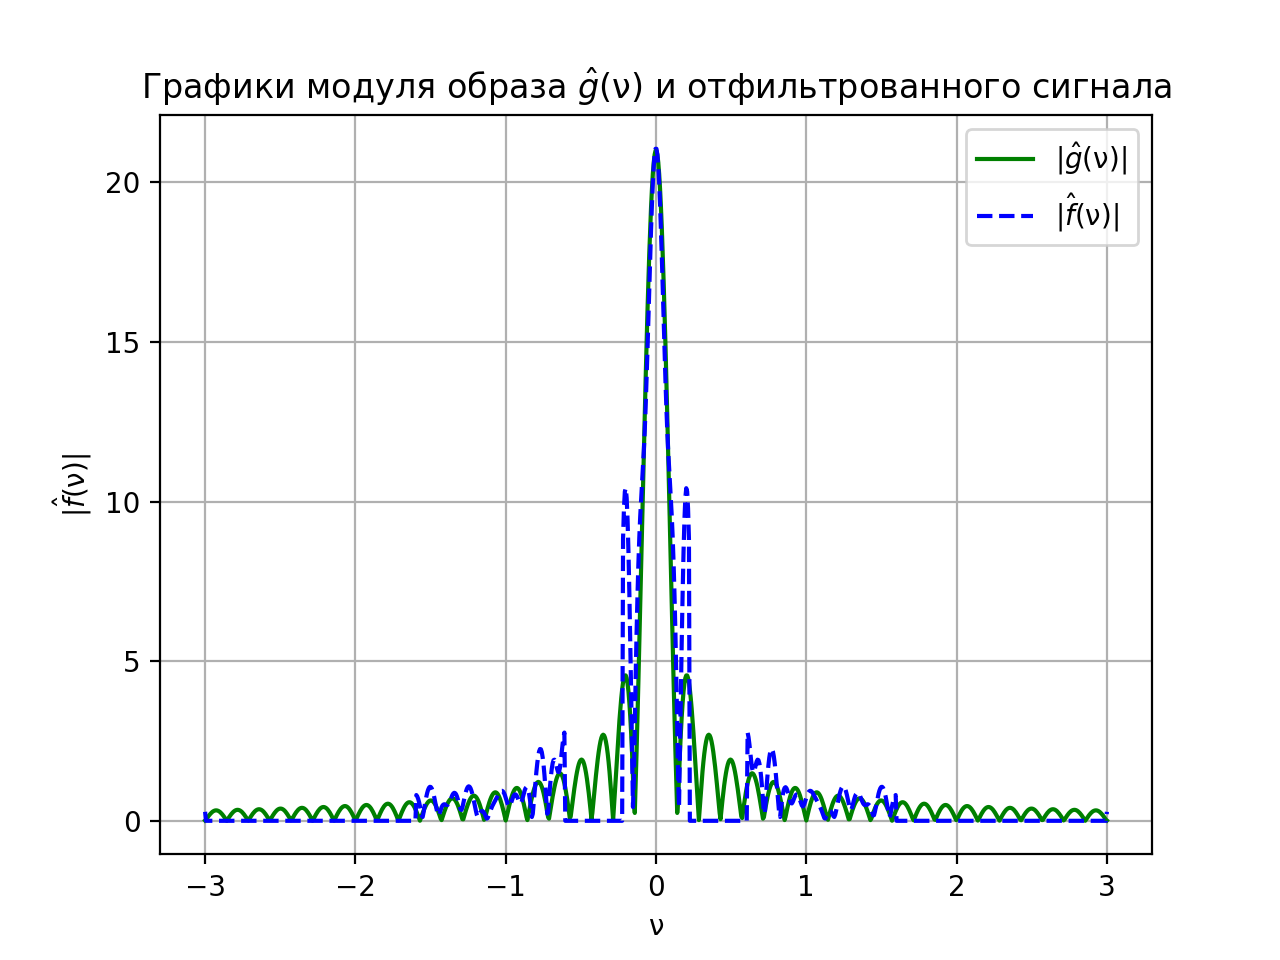
\includegraphics[scale=0.55]{media/1 task/specific_freq/Fourier_Image_Comparison_1_4_2_-0,6_-0,22_-2,99_-1,6.png}
    \caption{Сравнительные графики модулей Фурье-образа $g(t)$ и отфильтрованного сигнала при $b=1$,  $c=4$,  $d=2$}
    \label{fig:fourc_1_4_2}
\end{figure}

\begin{figure}[ht!]
    \centering
    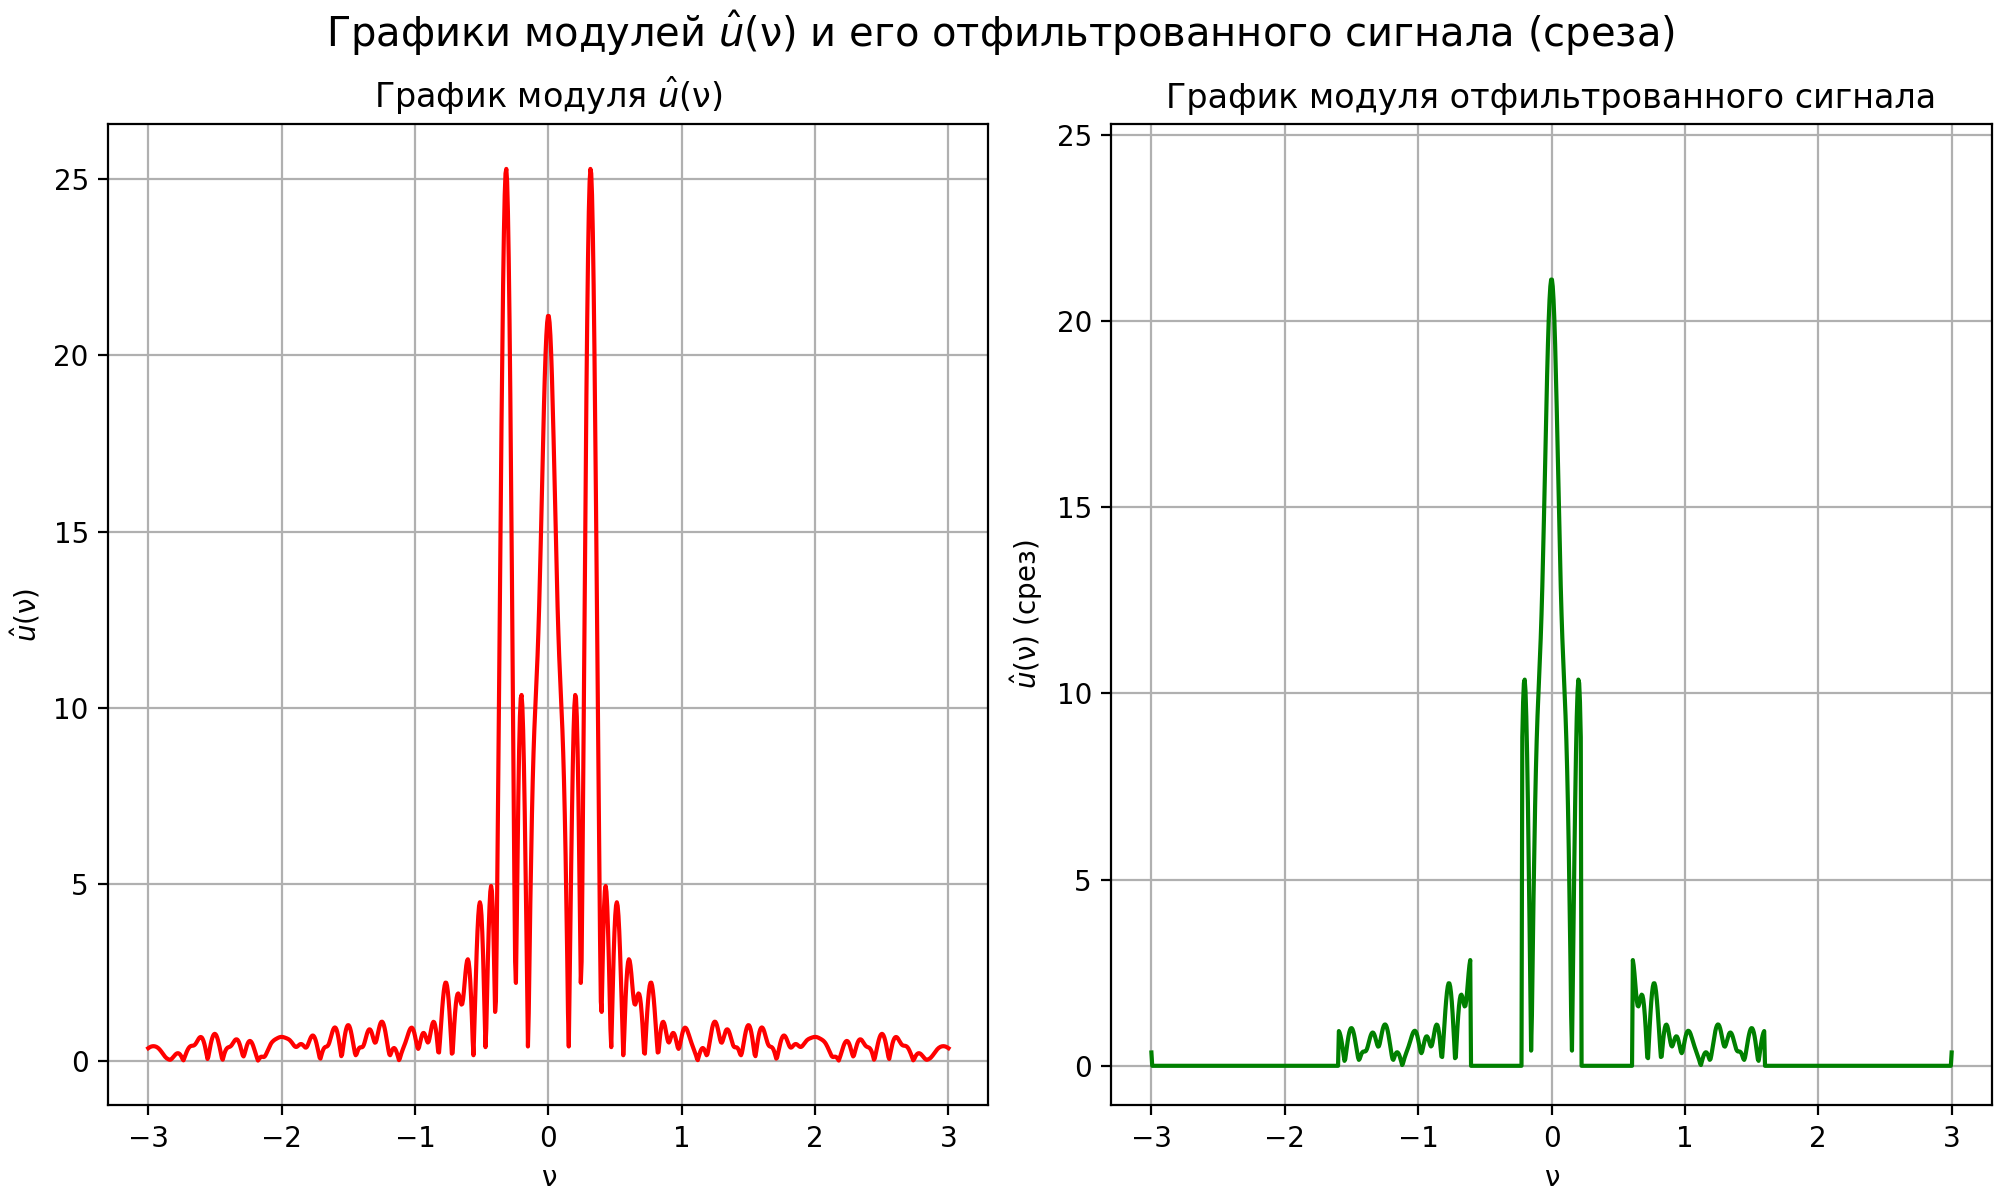
\includegraphics[scale=0.55]{media/1 task/specific_freq/Fourier_Image_2_4_2_-0,6_-0,22_-2,99_-1,6.png}
    \caption{Графики модулей Фурье-образа $u(t)$ и отфильтрованного сигнала при $b=2$,  $c=4$,  $d=2$}
    \label{fig:four_2_4_2}
\end{figure}

На графиках можно чётко проследить влияние параметра $b$ на Фурье-образ. При увеличении значения параметра мы видим, что значение модуля при некоторых частотах возрастает, при других --- уменьшается. В сравнении с графиками из пункта \ref{b_0} заметно появление хаотического шума.

\begin{figure}[ht!]
    \centering
    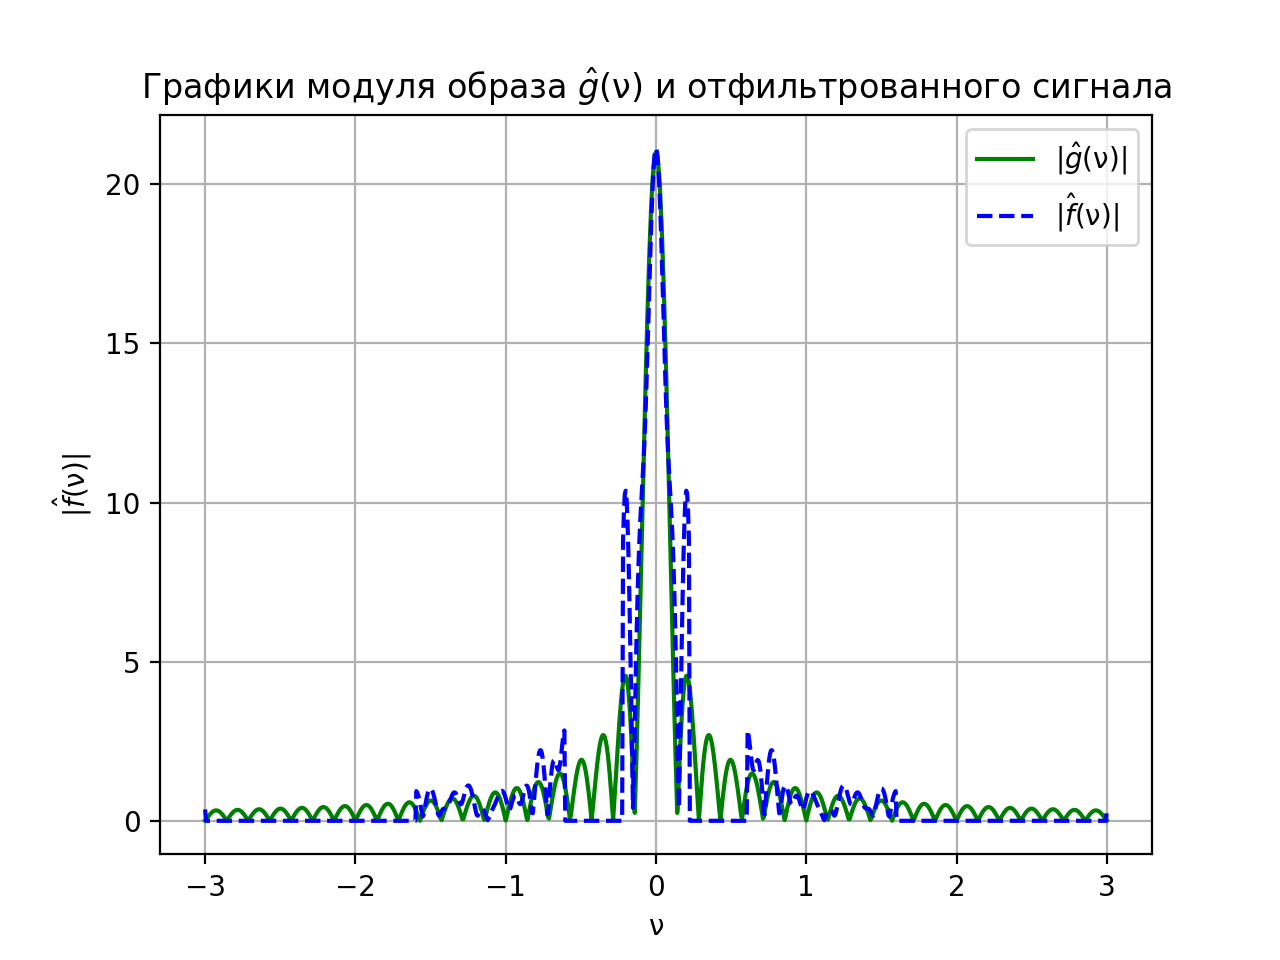
\includegraphics[scale=0.55]{media/1 task/specific_freq/Fourier_Image_Comparison_2_4_2_-0,6_-0,22_-2,99_-1,6.png}
    \caption{Сравнительные графики модулей Фурье-образа $g(t)$ и отфильтрованного сигнала при $b=2$,  $c=4$,  $d=2$}
    \label{fig:fourc_2_4_2}
\end{figure}



\begin{figure}[ht!]
    \centering
    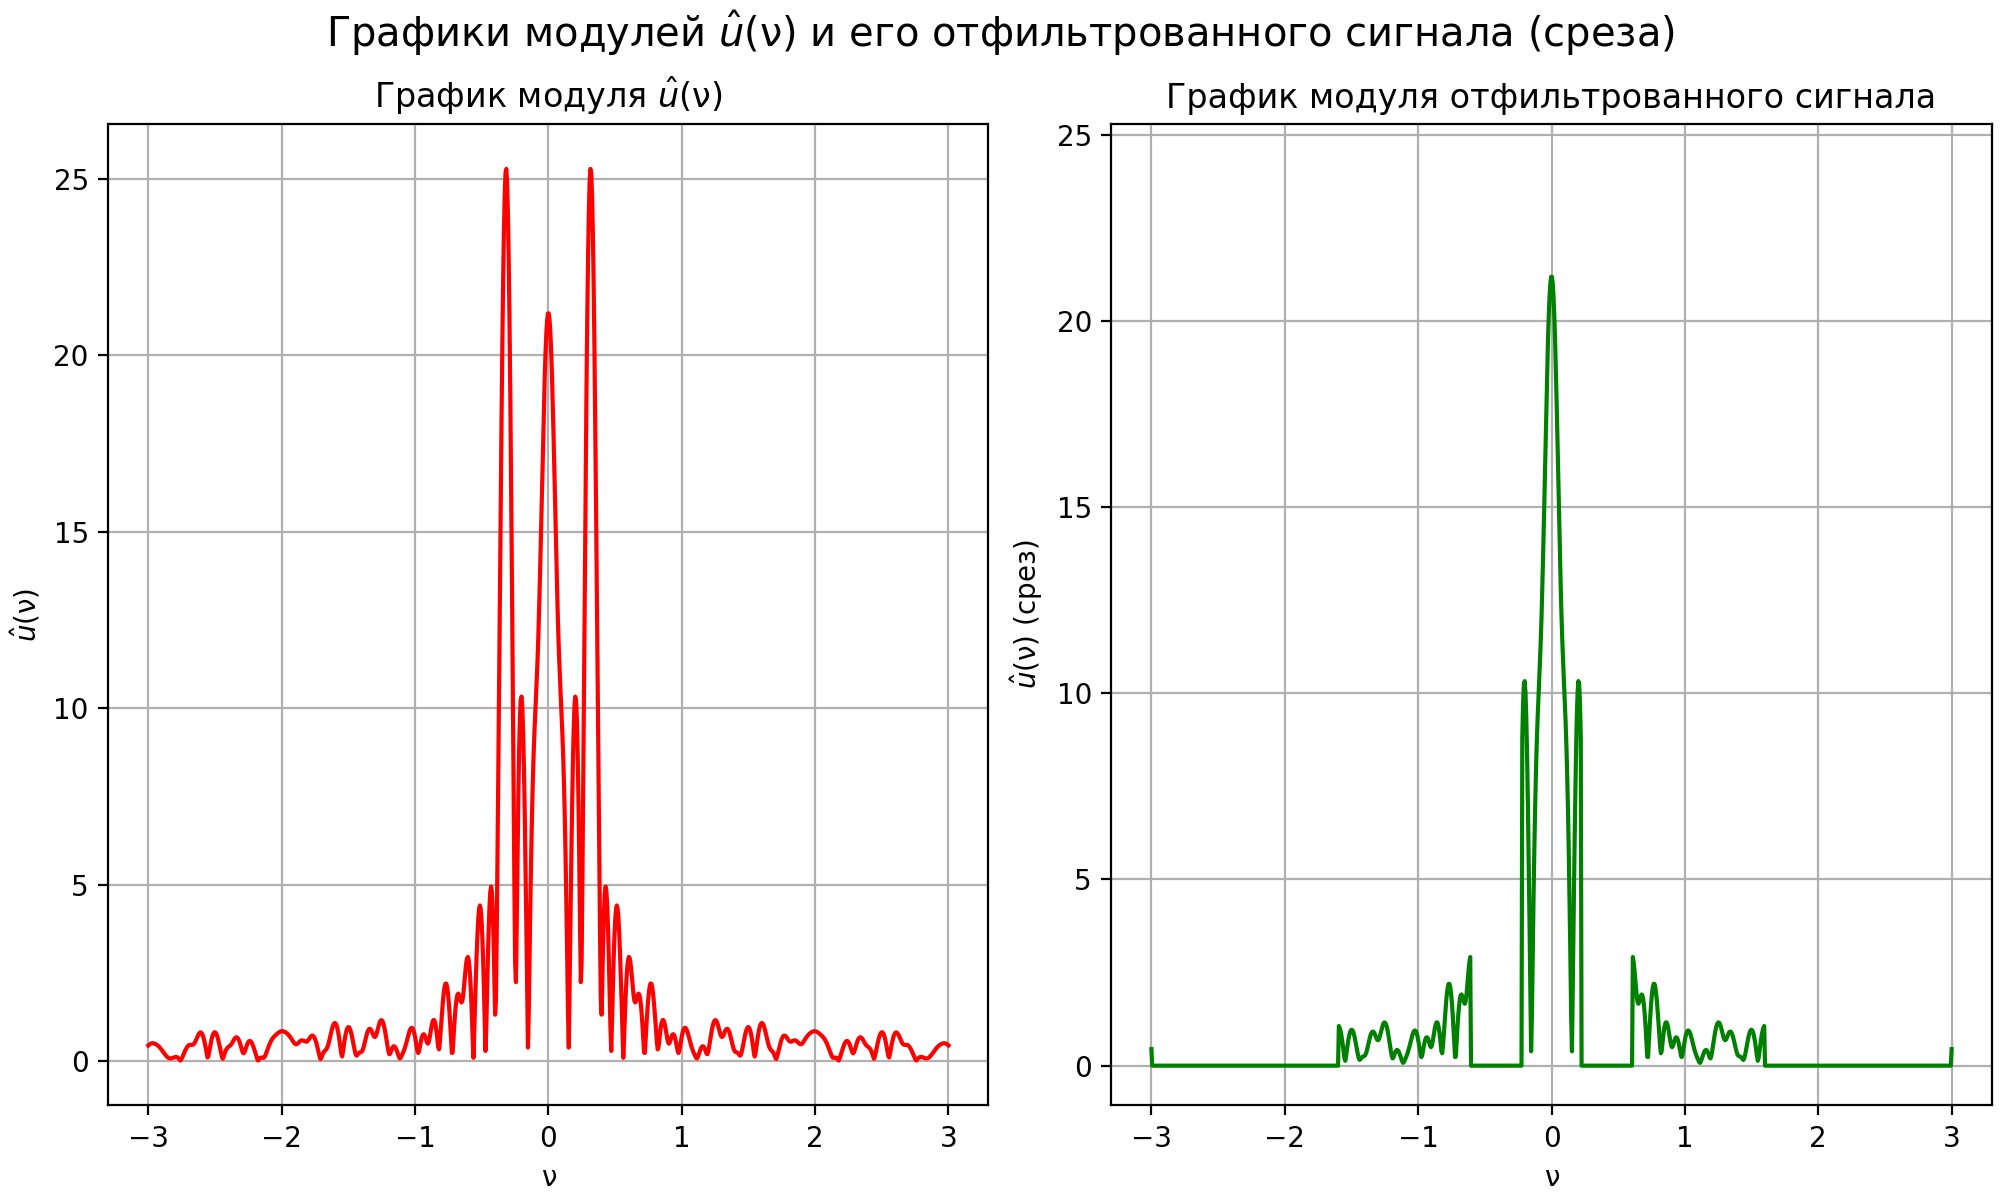
\includegraphics[scale=0.55]{media/1 task/specific_freq/Fourier_Image_3_4_2_-0,6_-0,22_-2,99_-1,6.png}
    \caption{Графики модулей Фурье-образа $f(t)$ и отфильтрованного сигнала при $b=3$,  $c=4$,  $d=2$}
    \label{fig:four_3_4_2}
\end{figure}

\begin{figure}[ht!]
    \centering
    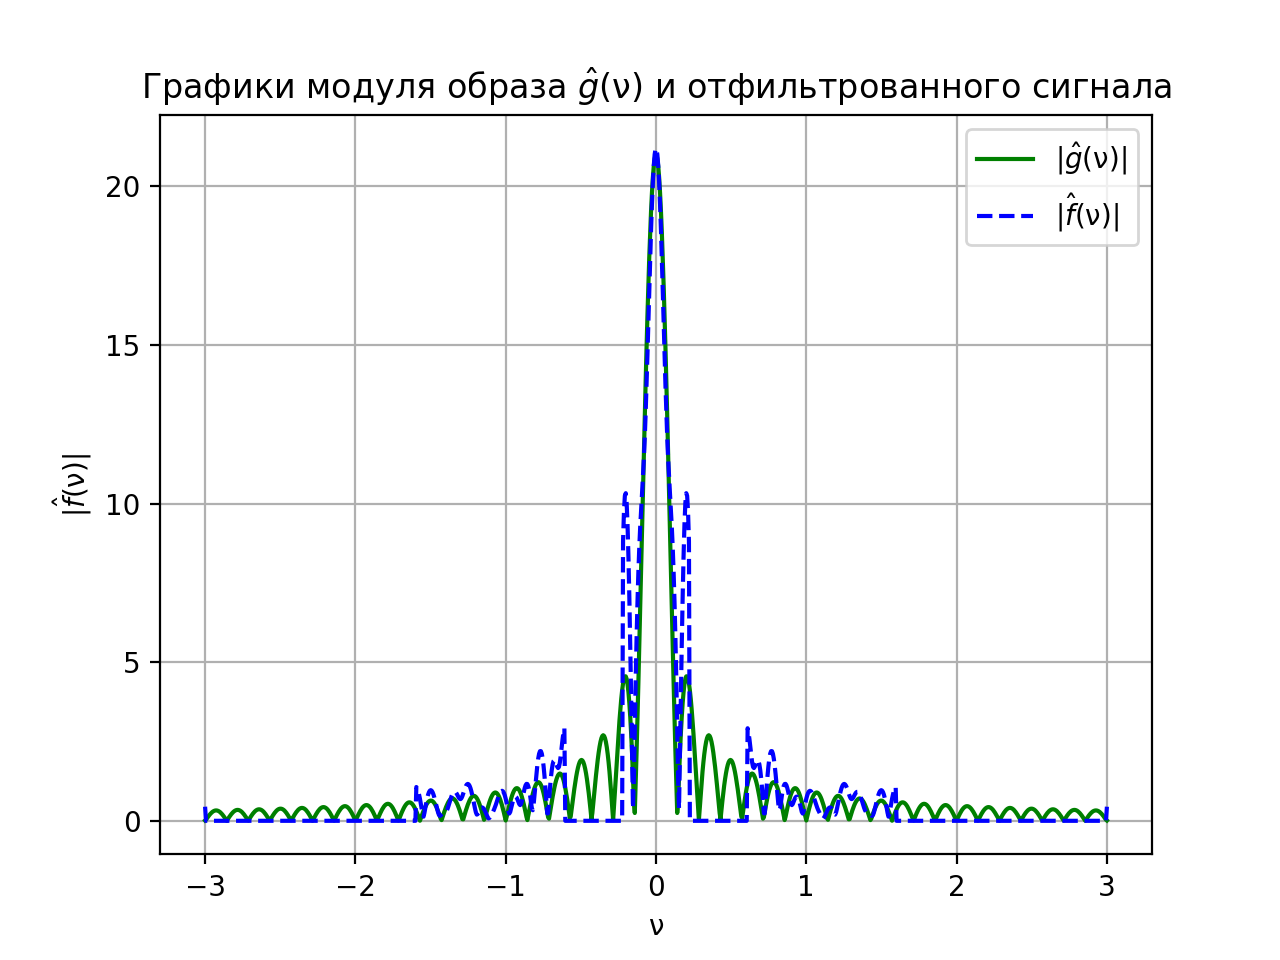
\includegraphics[scale=0.55]{media/1 task/specific_freq/Fourier_Image_Comparison_3_4_2_-0,6_-0,22_-2,99_-1,6.png}
    \caption{Сравнительные графики модулей Фурье-образа $g(t)$ и отфильтрованного сигнала при  $b=3$,  $c=4$,  $d=2$}
    \label{fig:fourc_3_4_2}
\end{figure}

\clearpage

\begin{figure}[ht!]
    \centering
    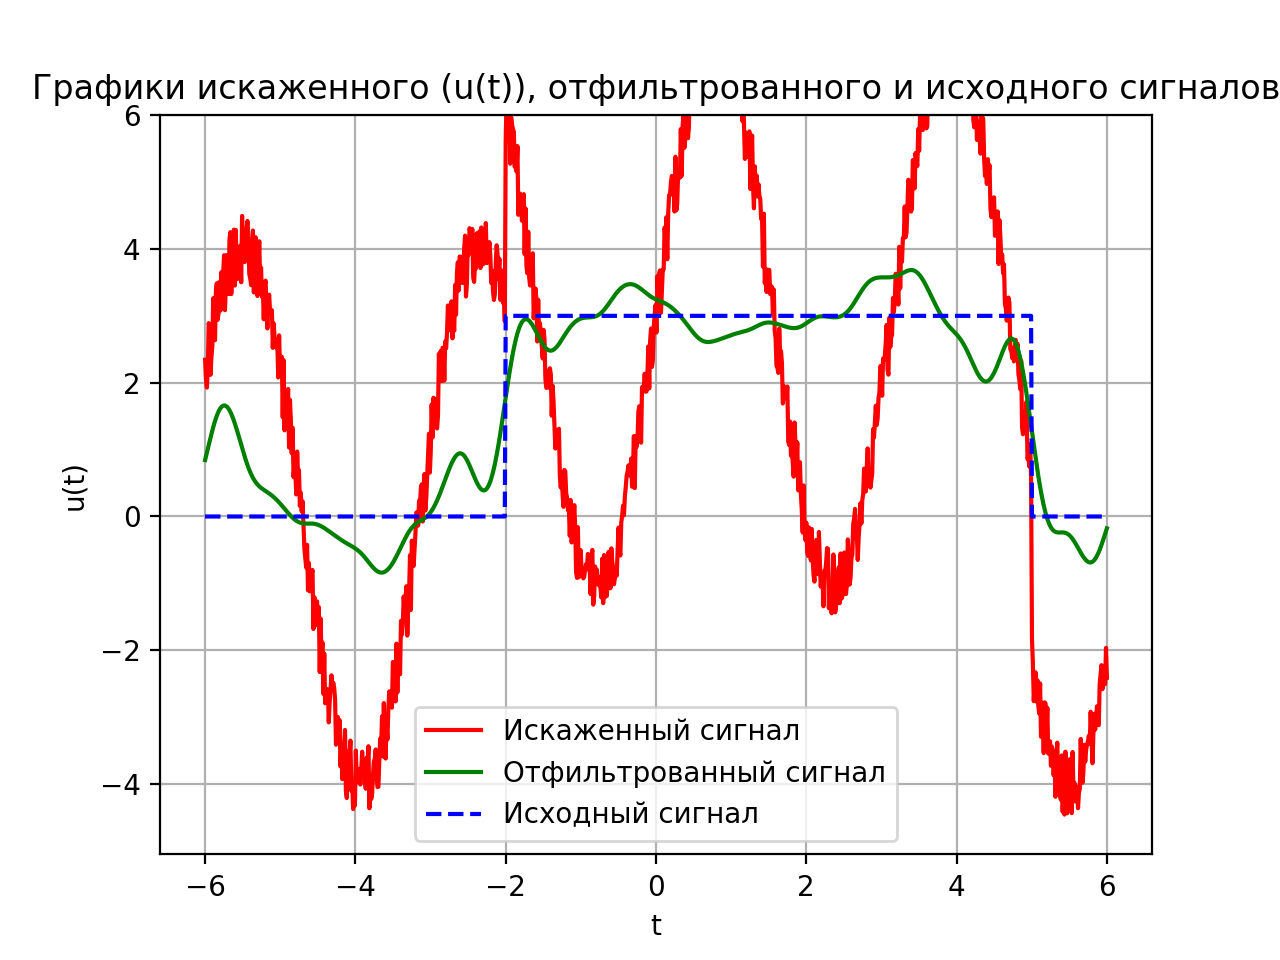
\includegraphics[scale=0.85]{media/1 task/specific_freq/Cleaned_1_4_2_-0,6_-0,22_-2,99_-1,6.png}
    \caption{Графики  $u(t)$, отфильтрованного и исходного сигналов при $b=1$,  $c=4$,  $d=2$}
    \label{fig:cleaned_1_4_2}
\end{figure}

\begin{figure}[ht!]
    \centering
    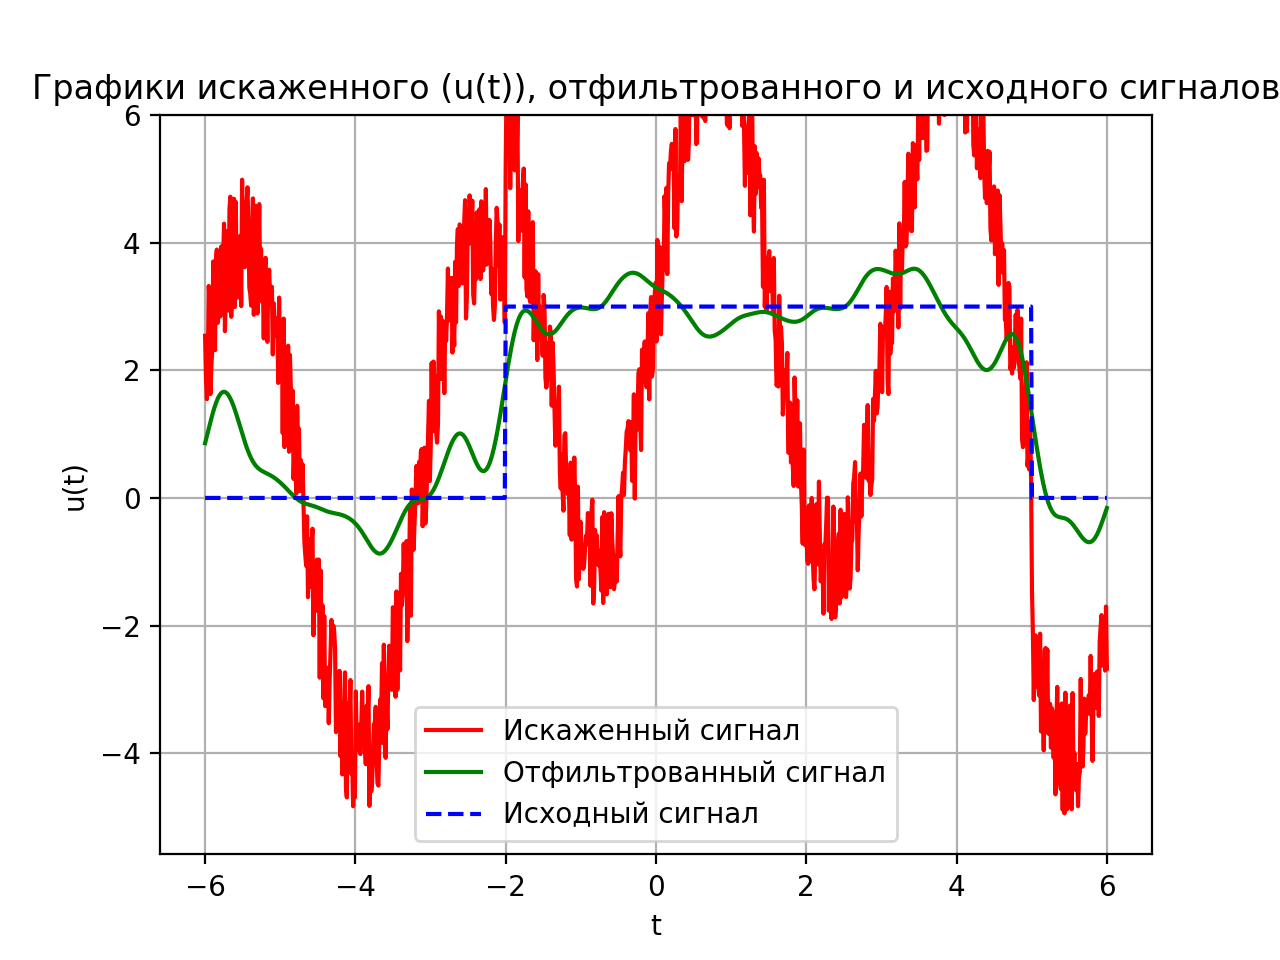
\includegraphics[scale=0.85]{media/1 task/specific_freq/Cleaned_2_4_2_-0,6_-0,22_-2,99_-1,6.png}
    \caption{Графики  $u(t)$, отфильтрованного и исходного сигналов при $b=2$,  $c=4$,  $d=2$}
    \label{fig:cleaned_2_4_2}
\end{figure}

\clearpage

\begin{figure}[ht!]
    \centering
    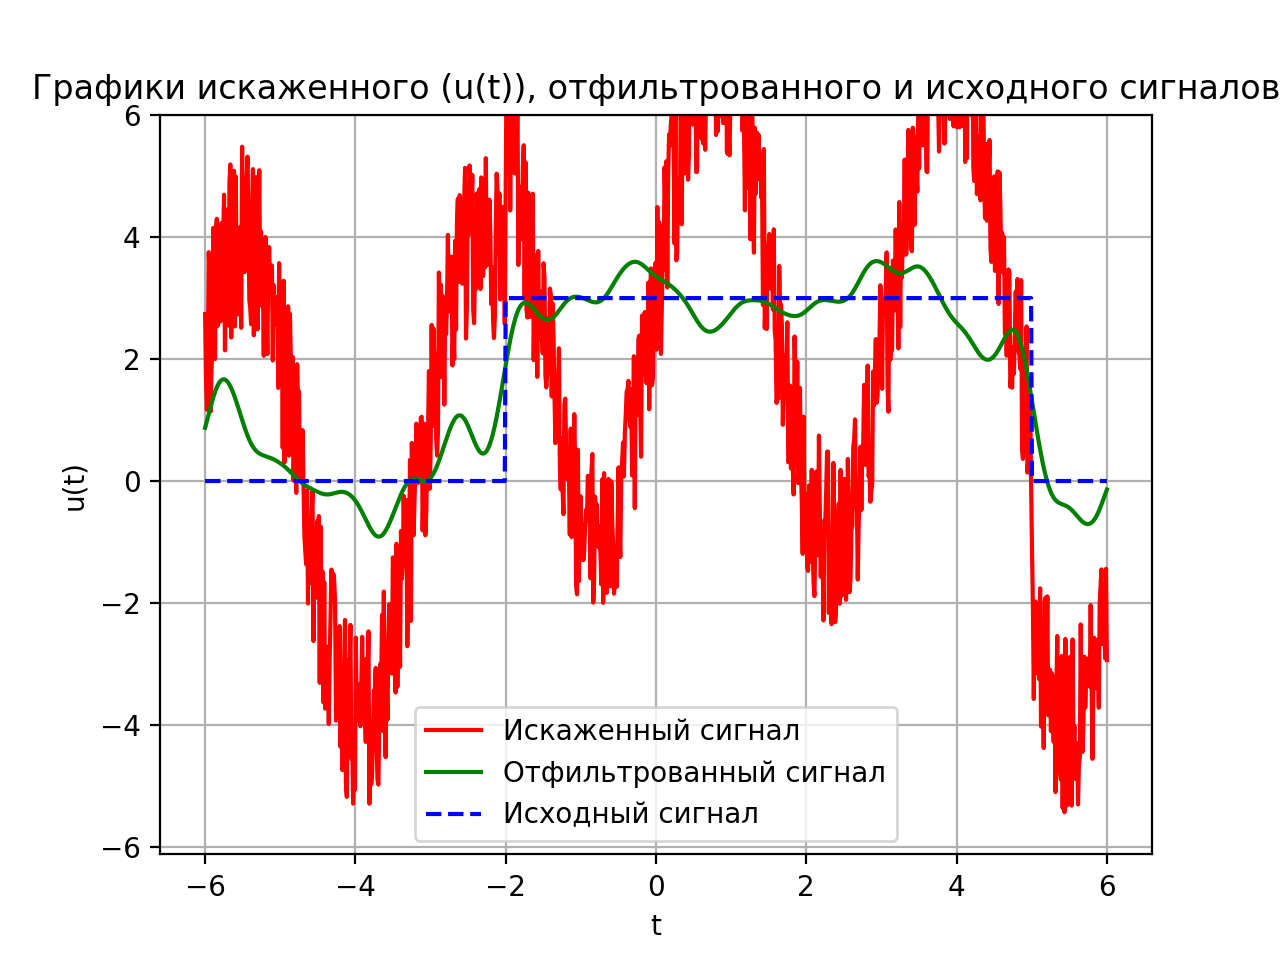
\includegraphics[scale=0.85]{media/1 task/specific_freq/Cleaned_3_4_2_-0,6_-0,22_-2,99_-1,6.png}
    \caption{Графики  $u(t)$, отфильтрованного и исходного сигналов при $b=3$,  $c=4$,  $d=2$}
    \label{fig:cleaned_3_4_2}
\end{figure}

При увеличении $b$, как говорилось ранее, увеличивается влияние хаотического шума, поэтому при одинаковом фильтрационном интервале отфильтрованный Фурье-образ начинает удаляться по норме от образа исходного сигнала (см. рисунки \ref{fig:fourc_1_4_2}, \ref{fig:fourc_2_4_2}, \ref{fig:fourc_3_4_2}). Это приводит к тому, что у отфильтрованного сигнала при одном и том же значении $t$ значение отфильтрованного сигнала начинает увеличиваться или уменьшаться.

\subsubsection{Подбираем правильные частоты среза }

Возьмём сигнал с параметрами $b=2, c=4, d=2$ из прошлого пункта \ref{b_ex}. График сигнала представлен на рисунке \ref{fig:noisy_2_4_2}. Нами уже был рассмотрен промежуток $\nu_0 \in [0.22, 0.6] \cup [1.6, 2.99]$. Теперь попробуем подобрать частоты таким образом, чтобы максимально приблизить его к исходному сигналу $g(t)$.

\clearpage

\begin{figure}[ht!]
    \centering
    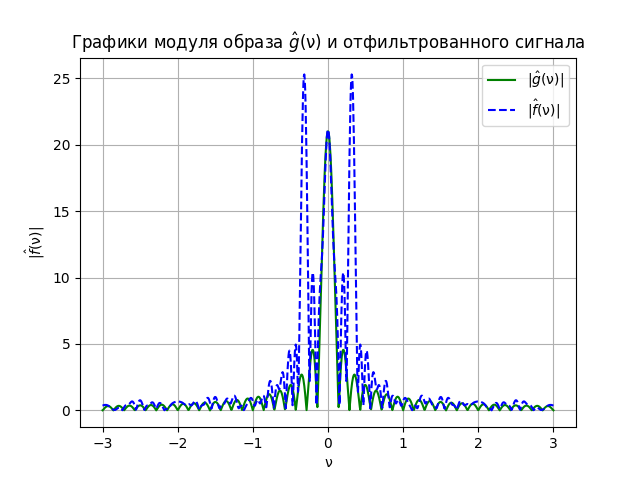
\includegraphics[scale=0.65]{media/1 task/specific_freq/Image_2_4_2_Begi.png}
    \caption{Сравнительные графики модулей Фурье-образа $g(t)$ и зашумленного сигнала при  $b=2$,  $c=4$,  $d=2$}
    \label{fig:fourcorig_2_4_2}
\end{figure}

Для начала уберём влияние синусоиды и поэкспериментируем с высокими частотами:

\begin{figure}[ht!]
    \centering
    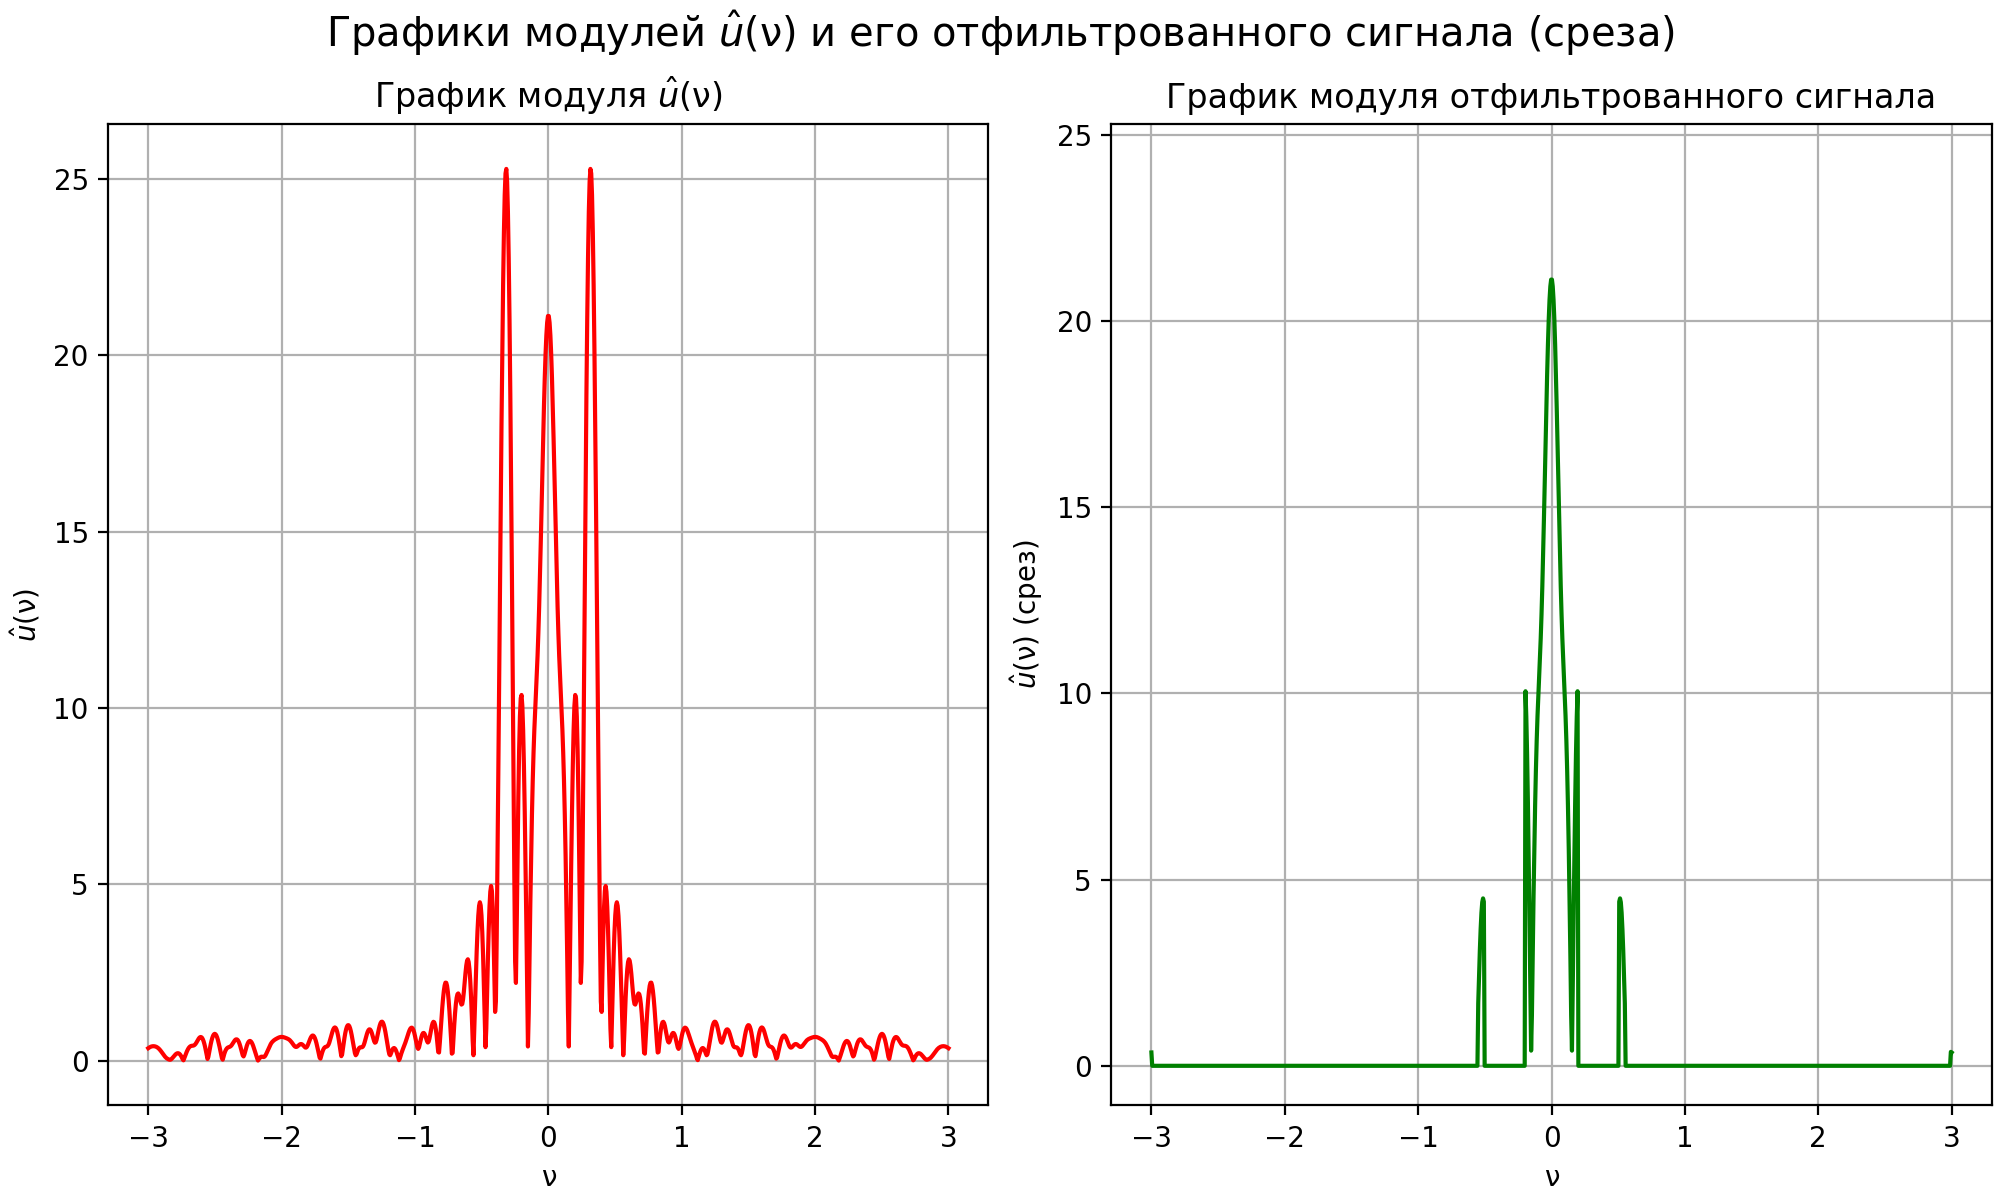
\includegraphics[scale=0.55]{media/1 task/specific_freq/Fourier_Image_2_4_2_-0,5_-0,2_-2,99_-0,55.png}
    \caption{Графики модулей Фурье-образа $u(t)$ и отфильтрованного сигнала при $b=2$, $c=4$, $d=2$; $\nu_0 \in [0.2, 0.5] \cup [0.55, 2.99]$}
    \label{fig:four_2_4_2_3}
\end{figure}

\clearpage

\begin{figure}[ht!]
    \centering
    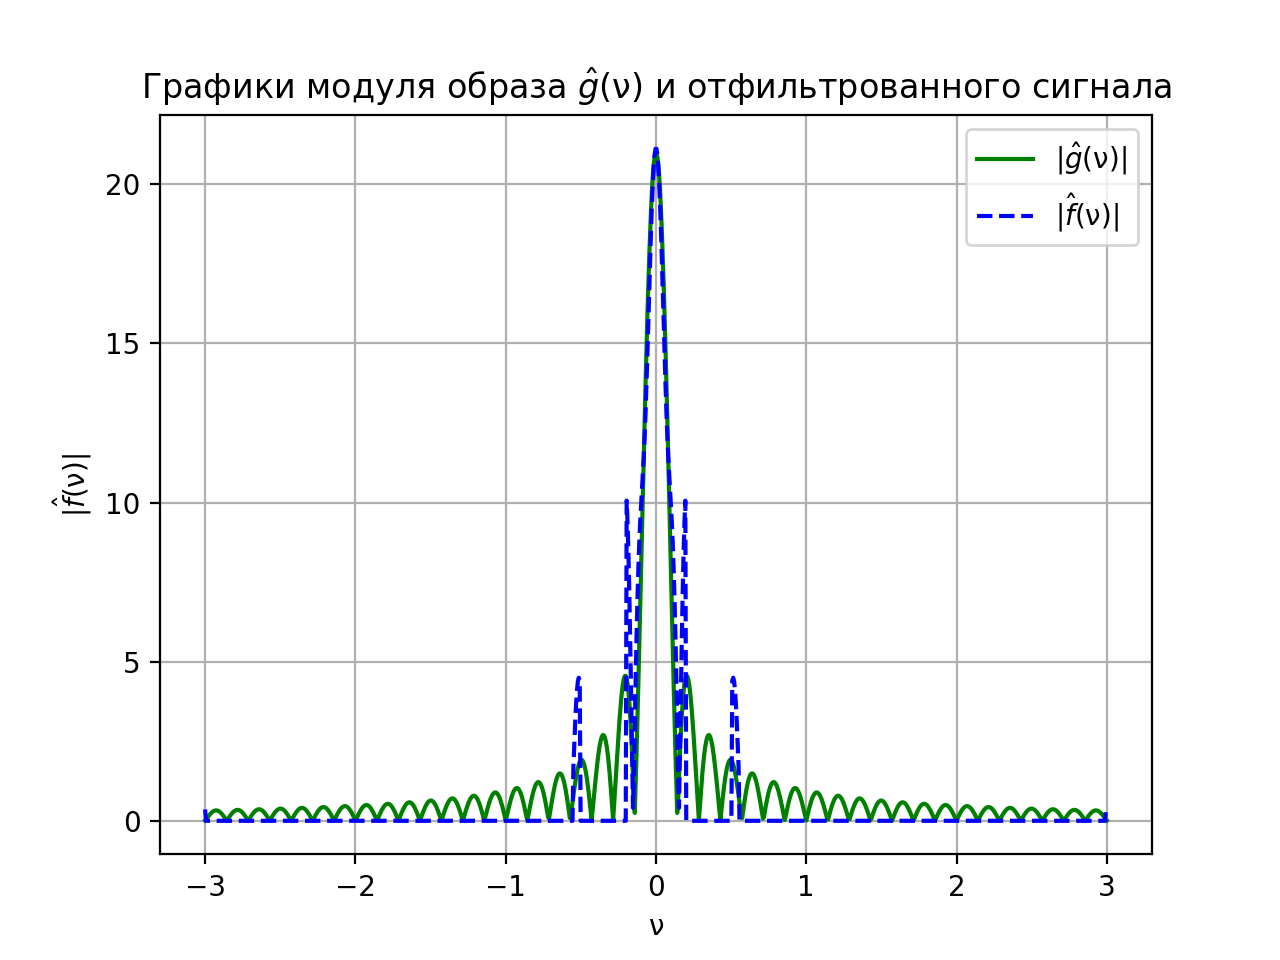
\includegraphics[scale=0.55]{media/1 task/specific_freq/Fourier_Image_Comparison_2_4_2_-0,5_-0,2_-2,99_-0,55.png}
    \caption{Сравнительные графики модулей Фурье-образа $g(t)$ и отфильтрованного сигнала при $b=2$, $c=4$, $d=2$; $\nu_0 \in [0.2, 0.5] \cup [0.55, 2.99]$}
    \label{fig:fourc_2_4_2_3}
\end{figure}

\begin{figure}[ht!]
    \centering
    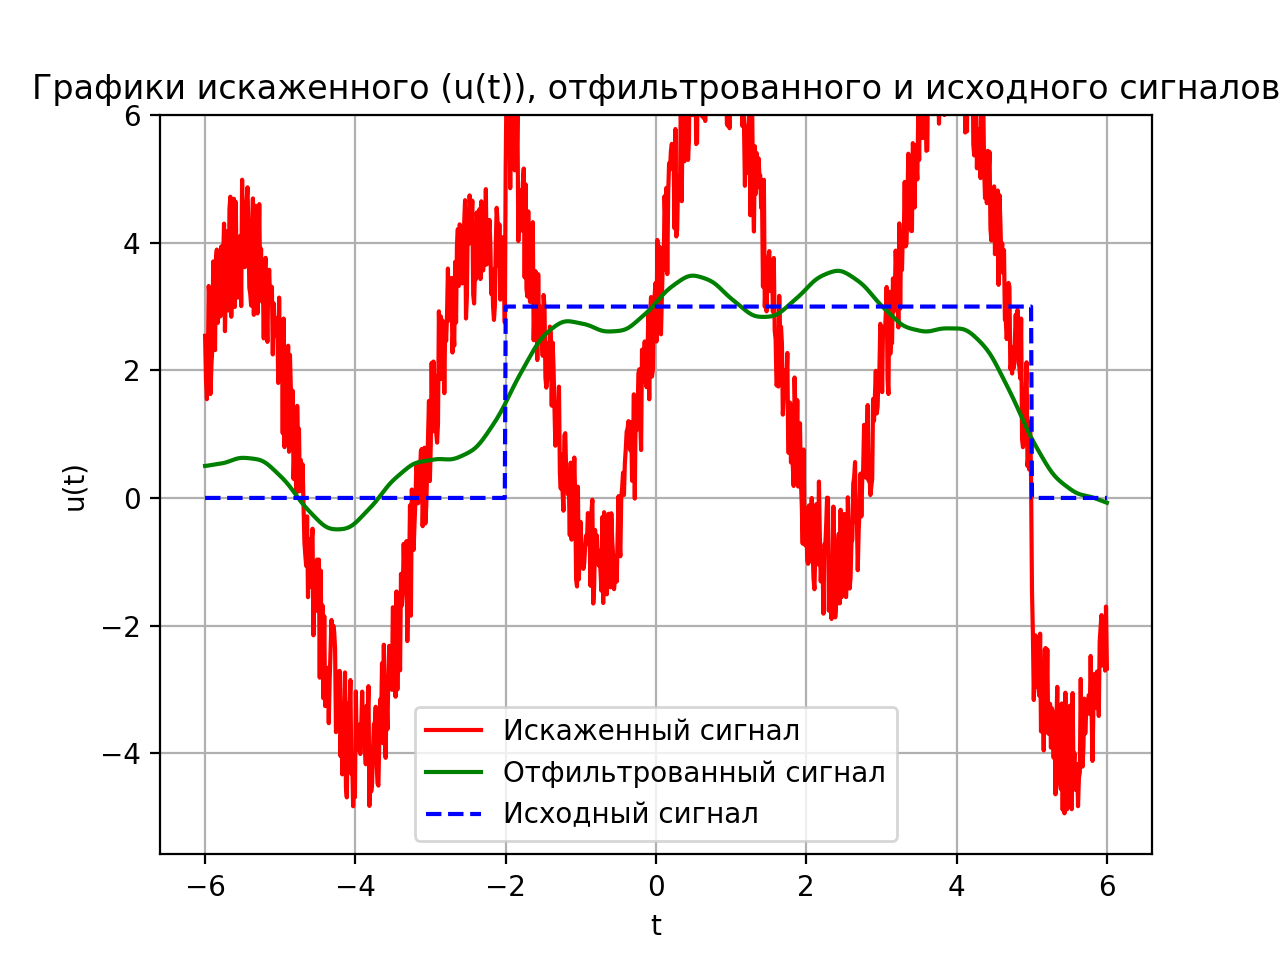
\includegraphics[scale=0.65]{media/1 task/specific_freq/Cleaned_2_4_2_-0,5_-0,2_-2,99_-0,55.png}
    \caption{Графики  $u(t)$, отфильтрованного и исходного сигналов при $b=2$, $c=4$, $d=2$; $\nu_0 \in [0.2, 0.5] \cup [0.55, 2.99]$}
    \label{fig:cleaned_2_4_2_3}
\end{figure}

\begin{figure}[ht!]
    \centering
    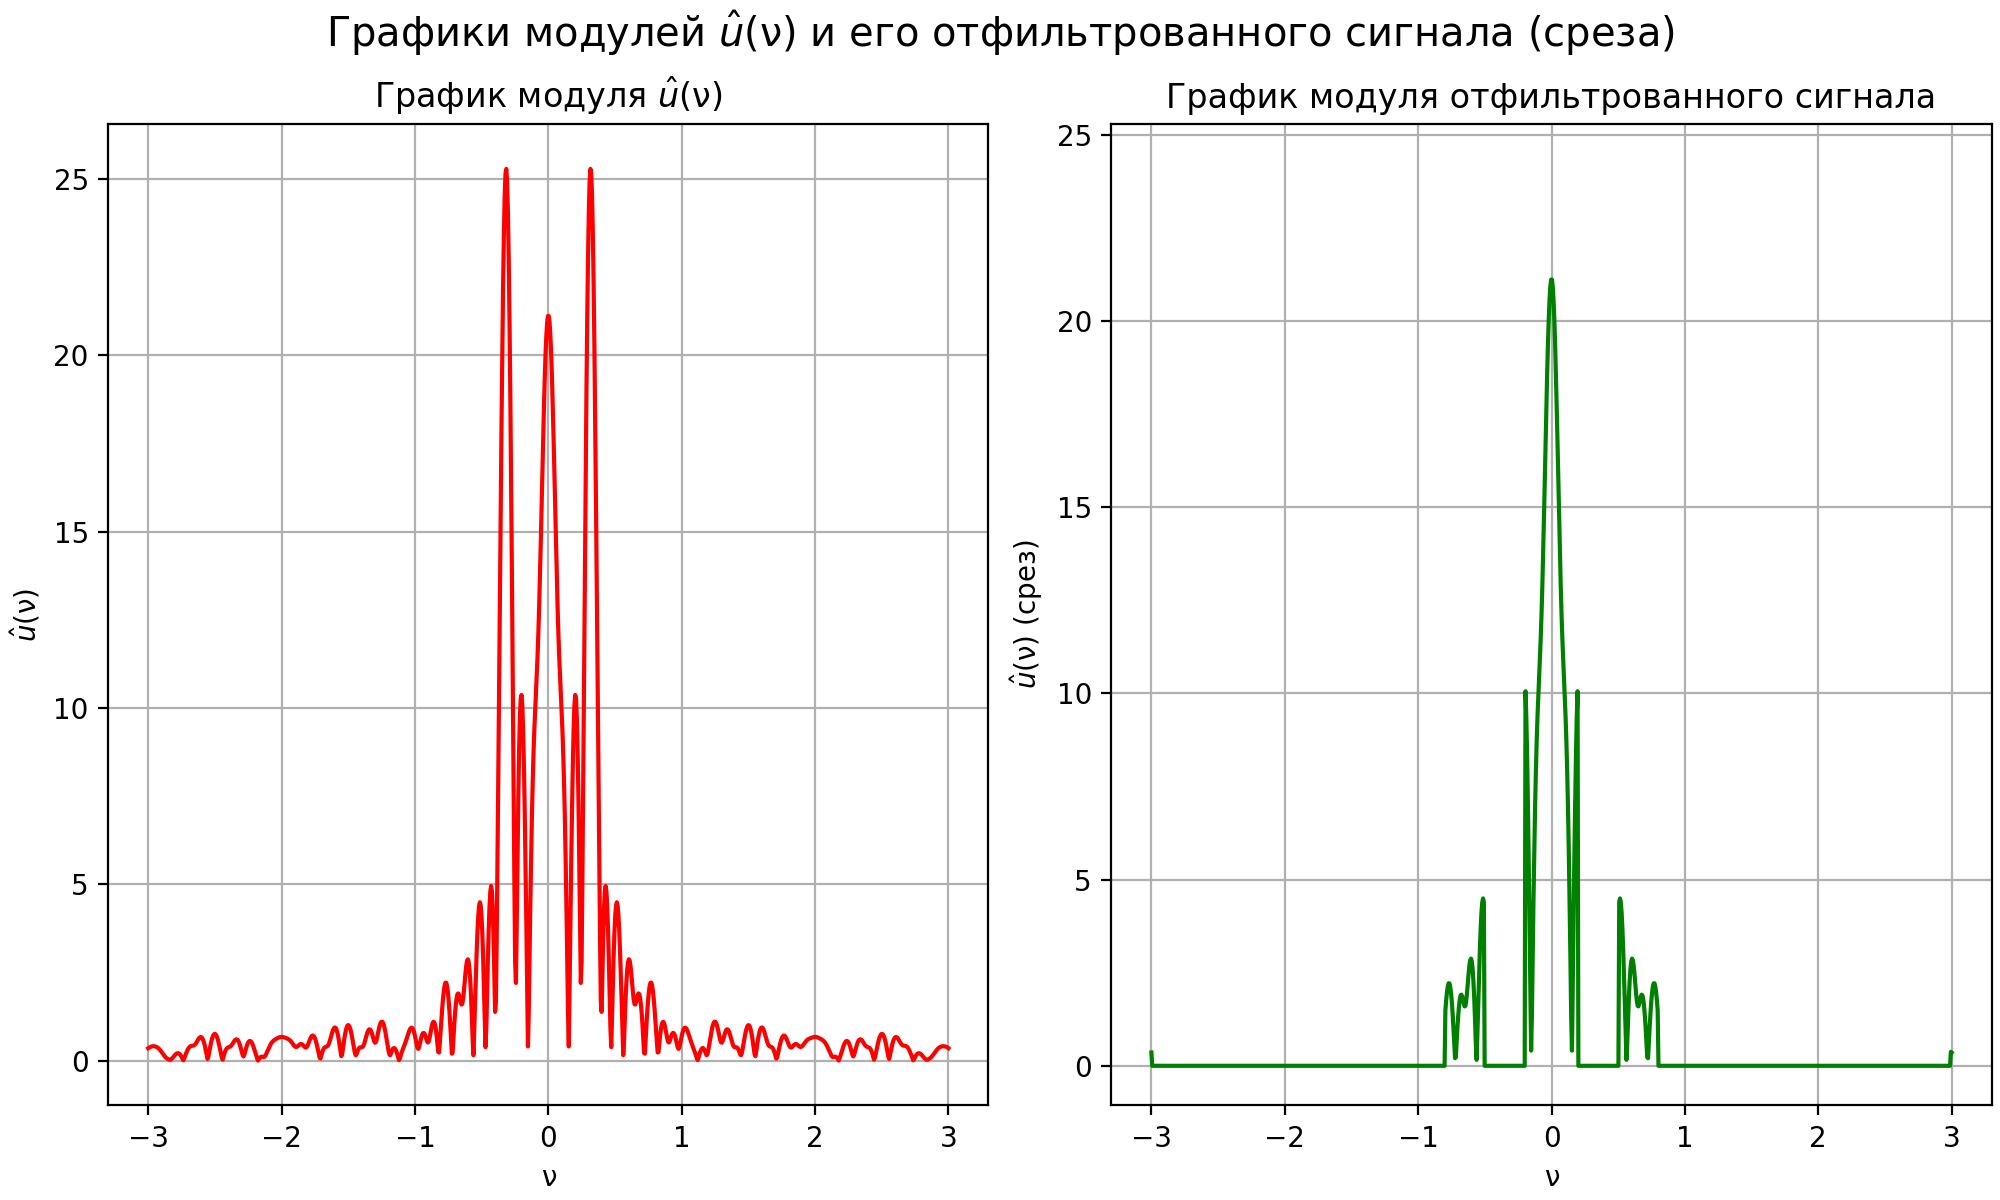
\includegraphics[scale=0.55]{media/1 task/specific_freq/Fourier_Image_2_4_2_-0,5_-0,2_-2,99_-0,8.png}
    \caption{Графики модулей Фурье-образа $u(t)$ и отфильтрованного сигнала при $b=2$, $c=4$, $d=2$; $\nu_0 \in [0.2, 0.5] \cup [0.8, 2.99]$}
    \label{fig:four_2_4_2_1}
\end{figure}

\begin{figure}[ht!]
    \centering
    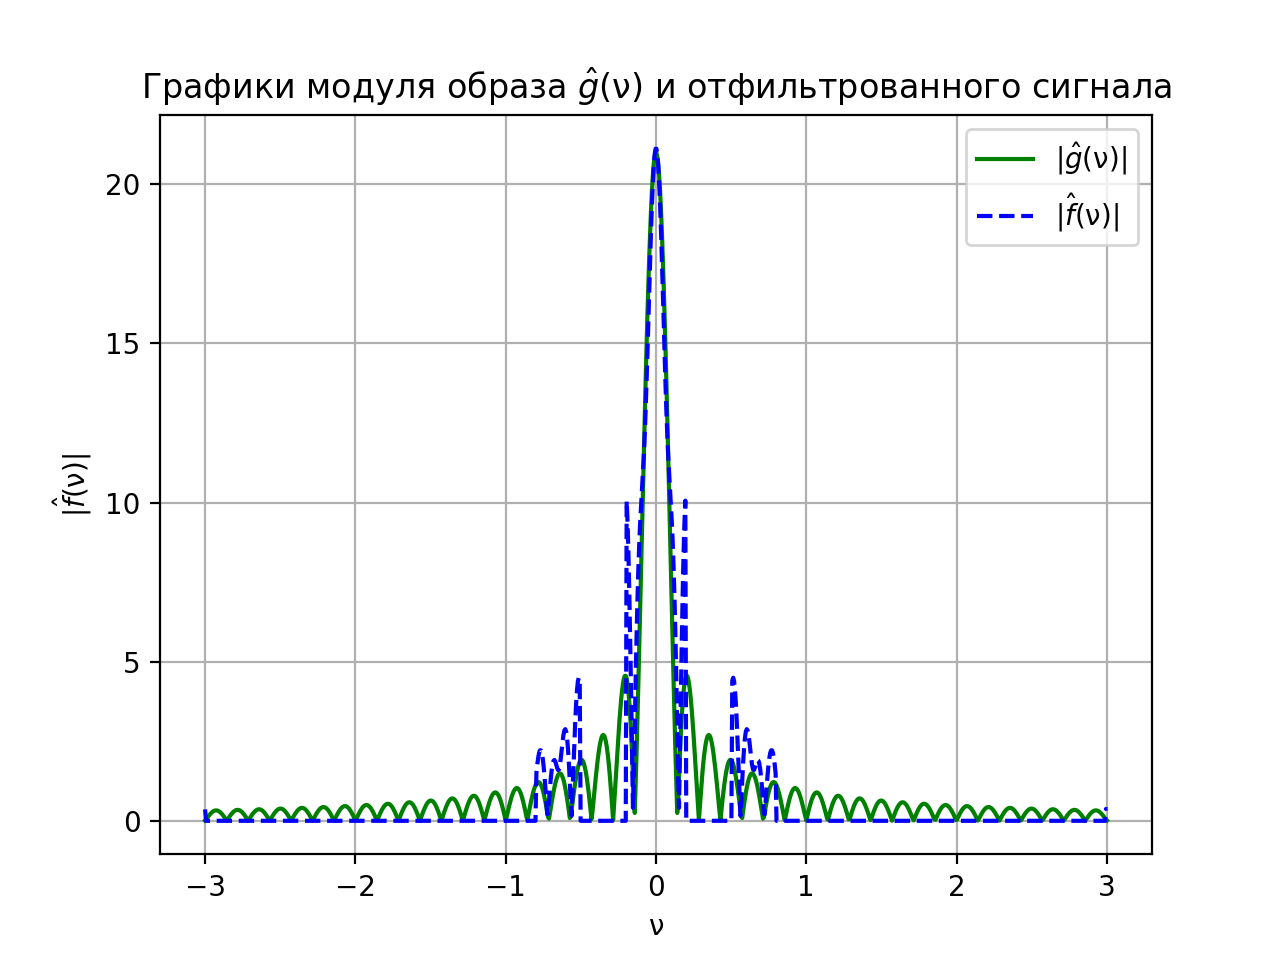
\includegraphics[scale=0.55]{media/1 task/specific_freq/Fourier_Image_Comparison_2_4_2_-0,5_-0,2_-2,99_-0,8.png}
    \caption{Сравнительные графики модулей Фурье-образа $g(t)$ и отфильтрованного сигнала при $b=2$, $c=4$, $d=2$; $\nu_0 \in [0.2, 0.5] \cup [0.8, 2.99]$}
    \label{fig:fourc_2_4_2_1}
\end{figure}

\begin{figure}[ht!]
    \centering
    \includegraphics[scale=0.65]{media/1 task/specific_freq/Cleaned_2_4_2_-0,5_-0,2_-2,99_-0,8.png}
    \caption{Графики  $u(t)$, отфильтрованного и исходного сигналов при $b=2$, $c=4$, $d=2$; $\nu_0 \in [0.2, 0.5] \cup [0.8, 2.99]$}
    \label{fig:cleaned_2_4_2_1}
\end{figure}

\begin{figure}[ht!]
    \centering
    \includegraphics[scale=0.55]{media/1 task/specific_freq/Fourier_Image_2_4_2_-0,5_-0,2_-2,99_-1,0.png}
    \caption{Графики модулей Фурье-образа $u(t)$ и отфильтрованного сигнала при $b=2$, $c=4$, $d=2$; $\nu_0 \in [0.2, 0.5] \cup [1.0, 2.99]$}
    \label{fig:four_2_4_2_2}
\end{figure}

\begin{figure}[ht!]
    \centering
    \includegraphics[scale=0.55]{media/1 task/specific_freq/Fourier_Image_Comparison_2_4_2_-0,5_-0,2_-2,99_-1,0.png}
    \caption{Сравнительные графики модулей Фурье-образа $g(t)$ и отфильтрованного сигнала при $b=2$, $c=4$, $d=2$; $\nu_0 \in [0.2, 0.5] \cup [1.0, 2.99]$}
    \label{fig:fourc_2_4_2_2}
\end{figure}

\begin{figure}[ht!]
    \centering
    \includegraphics[scale=0.65]{media/1 task/specific_freq/Cleaned_2_4_2_-0,5_-0,2_-2,99_-1,0.png}
    \caption{Графики  $u(t)$, отфильтрованного и исходного сигналов при $b=2$, $c=4$, $d=2$; $\nu_0 \in [0.2, 0.5] \cup [1.0, 2.99]$}
    \label{fig:cleaned_2_4_2_2}
\end{figure}

\clearpage

Нам удалось получить приемлимый результат. Важно отметить, что при уменьшении левой границы интервала для фильтрации высоких частот мы сглаживаем график отфильтрованного сигнала, но при чрезмерном уменьшении частоты среза колебания начинают увеличиваться, так как у нас остаётся небольшая окрестность частоты, с которой начинает колебаться сигнал (рисунок \ref{fig:cleaned_2_4_2_3}).

Теперь попробуем увеличить диапазон частот, которые мы исключаем для избавления от синусоидальных шумов ($\nu_0 \in [0.2, 1.2]$):

\vfill

\begin{figure}[ht!]
    \centering
    \includegraphics[scale=0.55]{media/1 task/specific_freq/Fourier_Image_2_4_2_-1,2_-0,2_-2,99_-2,7_-2,7_-1,7.png}
    \caption{Графики модулей Фурье-образа $u(t)$ и отфильтрованного сигнала при $b=2$, $c=4$, $d=2$; $\nu_0 \in [0.2, 1.2] \cup [1.7, 2.99]$}
    \label{fig:four_2_4_2_4}
\end{figure}

\begin{figure}[ht!]
    \centering
    \includegraphics[scale=0.55]{media/1 task/specific_freq/Fourier_Image_Comparison_2_4_2_-1,2_-0,2_-2,99_-2,7_-2,7_-1,7.png}
    \caption{Сравнительные графики модулей Фурье-образа $g(t)$ и отфильтрованного сигнала при $b=2$, $c=4$, $d=2$; $\nu_0 \in [0.2, 1.2] \cup [1.7, 2.99]$}
    \label{fig:fourc_2_4_2_4}
\end{figure}

\begin{figure}[ht!]
    \centering
    \includegraphics[scale=0.65]{media/1 task/specific_freq/Cleaned_2_4_2_-1,2_-0,2_-2,99_-2,7_-2,7_-1,7.png}
    \caption{Графики  $u(t)$, отфильтрованного и исходного сигналов при $b=2$, $c=4$, $d=2$; $\nu_0 \in [0.2, 1.2] \cup [1.7, 2.99]$}
    \label{fig:cleaned_2_4_2_4}
\end{figure}

\begin{figure}[ht!]
    \centering
    \includegraphics[scale=0.55]{media/1 task/specific_freq/Fourier_Image_2_4_2_-1,2_-0,2_-2,99_-2,7_-2,7_-1,5.png}
    \caption{Графики модулей Фурье-образа $u(t)$ и отфильтрованного сигнала при $b=2$, $c=4$, $d=2$; $\nu_0 \in [0.2, 1.2] \cup [1.5, 2.99]$}
    \label{fig:four_2_4_2_5}
\end{figure}

\begin{figure}[ht!]
    \centering
    \includegraphics[scale=0.55]{media/1 task/specific_freq/Fourier_Image_Comparison_2_4_2_-1,2_-0,2_-2,99_-2,7_-2,7_-1,5.png}
    \caption{Сравнительные графики модулей Фурье-образа $g(t)$ и отфильтрованного сигнала при $b=2$, $c=4$, $d=2$; $\nu_0 \in [0.2, 1.2] \cup [1.5, 2.99]$}
    \label{fig:fourc_2_4_2_5}
\end{figure}

\begin{figure}[ht!]
    \centering
    \includegraphics[scale=0.65]{media/1 task/specific_freq/Cleaned_2_4_2_-1,2_-0,2_-2,99_-2,7_-2,7_-1,5.png}
    \caption{Графики  $u(t)$, отфильтрованного и исходного сигналов при $b=2$, $c=4$, $d=2$; $\nu_0 \in [0.2, 1.2] \cup [1.5, 2.99]$}
    \label{fig:cleaned_2_4_2_5}
\end{figure}

\begin{figure}[ht!]
    \centering
    \includegraphics[scale=0.55]{media/1 task/specific_freq/Fourier_Image_2_4_2_-1,2_-0,2_-2,99_-2,7_-2,7_-1,3.png}
    \caption{Графики модулей Фурье-образа $u(t)$ и отфильтрованного сигнала при $b=2$, $c=4$, $d=2$; $\nu_0 \in [0.2, 1.2] \cup [1.3, 2.99]$}
    \label{fig:four_2_4_2_6}
\end{figure}

\begin{figure}[ht!]
    \centering
    \includegraphics[scale=0.55]{media/1 task/specific_freq/Fourier_Image_Comparison_2_4_2_-1,2_-0,2_-2,99_-2,7_-2,7_-1,3.png}
    \caption{Сравнительные графики модулей Фурье-образа $g(t)$ и отфильтрованного сигнала при $b=2$, $c=4$, $d=2$; $\nu_0 \in [0.2, 1.2] \cup [1.3, 2.99]$}
    \label{fig:fourc_2_4_2_6}
\end{figure}

\begin{figure}[ht!]
    \centering
    \includegraphics[scale=0.65]{media/1 task/specific_freq/Cleaned_2_4_2_-1,2_-0,2_-2,99_-2,7_-2,7_-1,3.png}
    \caption{Графики  $u(t)$, отфильтрованного и исходного сигналов при $b=2$, $c=4$, $d=2$; $\nu_0 \in [0.2, 1.2] \cup [1.3, 2.99]$}
    \label{fig:cleaned_2_4_2_6}
\end{figure}

\clearpage

Увеличение диапазона низких частот приводит к сглаживанию скачков при $t=-2, 5$. При увеличении диапазона высоких частот для фильтрации мы приходим выводу, аналогичному для рисунков \ref{fig:cleaned_2_4_2_3}, \ref{fig:cleaned_2_4_2_1}, \ref{fig:cleaned_2_4_2_2}.

После фильтрации зашумленного сигнала при разных частотах среза можно сказать, что отбрасывание нескольких диапазонов частот заметно сглаживает шумы и позволяет приблизить сигнал к исходному и мы позволяет определить примерый вид сигнала $g(t)$. Можно предположить, что для более точного приближения необходимо <<обнулять>> меньшие окрестности определённых частот. Но при уменьшении диапазона высоких частот можно наблюдать увеличение колебаний сигнала, поэтому нельзя однозначно утверждать, что возможно полное избавление от шумов и приведение сигнала к исходному.
\clearpage

\subsection{Низкие частоты}

Возьмём сигнал с параметрами $b=4$ $c=2$ $d=2$, график которого приведён ниже:

\begin{figure}[ht!]
    \centering
    \includegraphics[scale=0.5]{media/1 task/low_freq/Noisy_4_2_2.png}
    \caption{График $u(t)$ при $b=4$, $c=2$ и $d=2$}
    \label{fig:noisy_4_2_2}
\end{figure}

\subsubsection{Частоты, частоты и ещё раз частоты!}

В качестве частоты среза будут выступать значения $0.4, 0.6, 1.2, 1.8$ Гц. Графики приведены ниже:

\begin{figure}[ht!]
    \centering
    \includegraphics[scale=0.5]{media/1 task/low_freq/Fourier_Image_4_2_2_-0,4.png}
    \caption{Графики модулей Фурье-образа $u(t)$ и отфильтрованного сигнала при $\nu_0=0.4$ Гц}
    \label{fig:four_4_2_2_0.4}
\end{figure}

\begin{figure}[ht!]
    \centering
    \includegraphics[scale=0.55]{media/1 task/low_freq/Fourier_Image_Comparison_4_2_2_-0,4.png}
    \caption{Сравнительные графики модулей Фурье-образа $g(t)$ и отфильтрованного сигнала при $\nu_0=0.4$ Гц}
    \label{fig:fourc_4_2_2_0.4}
\end{figure}

\begin{figure}[ht!]
    \centering
    \includegraphics[scale=0.55]{media/1 task/low_freq/Fourier_Image_4_2_2-0,5975975975975976.png}
    \caption{Графики модулей Фурье-образа $u(t)$ и отфильтрованного сигнала при $\nu_0=0.6$ Гц}
    \label{fig:four_4_2_2_0.6}
\end{figure}

\begin{figure}[ht!]
    \centering
    \includegraphics[scale=0.55]{media/1 task/low_freq/Fourier_Image_Comparison_4_2_2-0,5975975975975976.png}
    \caption{Сравнительные графики модулей Фурье-образа $g(t)$ и отфильтрованного сигнала при $\nu_0=0.6$ Гц}
    \label{fig:fourc_4_2_2_0.6}
\end{figure}

\begin{figure}[ht!]
    \centering
    \includegraphics[scale=0.55]{media/1 task/low_freq/Fourier_Image_4_2_2-1,1981981981981982.png}
    \caption{Графики модулей Фурье-образа $u(t)$ и отфильтрованного сигнала при $\nu_0=1.2$ Гц}
    \label{fig:four_4_2_2_1.2}
\end{figure}

\begin{figure}[ht!]
    \centering
    \includegraphics[scale=0.55]{media/1 task/low_freq/Fourier_Image_Comparison_4_2_2-1,1981981981981982.png}
    \caption{Сравнительные графики модулей Фурье-образа $g(t)$ и отфильтрованного сигнала при $\nu_0=1.2$ Гц}
    \label{fig:fourc_4_2_2_1.2}
\end{figure}

\begin{figure}[ht!]
    \centering
    \includegraphics[scale=0.55]{media/1 task/low_freq/Fourier_Image_4_2_2-1,7987987987987988.png}
    \caption{Графики модулей Фурье-образа $u(t)$ и отфильтрованного сигнала при $\nu_0=1.8$ Гц}
    \label{fig:four_4_2_2_1.8}
\end{figure}

\clearpage

\begin{figure}[ht!]
    \centering
    \includegraphics[scale=0.55]{media/1 task/low_freq/Fourier_Image_Comparison_4_2_2-1,7987987987987988.png}
    \caption{Сравнительные графики модулей Фурье-образа $g(t)$ и отфильтрованного сигнала при $\nu_0=1.8$ Гц}
    \label{fig:fourc_4_2_2_1.8}
\end{figure}


Каждый раз мы берём всё более высокую частоту среза. Посмотрим, как это отразиться на фильтрации:

\begin{figure}[ht!]
    \centering
    \includegraphics[scale=0.75]{media/1 task/low_freq/Cleaned_4_2_2_-0,4.png}
    \caption{Графики  $u(t)$, отфильтрованного и исходного сигналов при $\nu_0=0.4$ Гц}
    \label{fig:cleaned_4_2_2_0.4}
\end{figure}

\clearpage

\begin{figure}[ht!]
    \centering
    \includegraphics[scale=0.75]{media/1 task/low_freq/Cleaned_4_2_2_-0,5975975975975976.png}
    \caption{Графики  $u(t)$, отфильтрованного и исходного сигналов при $\nu_0=0.6$ Гц}
    \label{fig:cleaned_4_2_2_0.6}
\end{figure}

\begin{figure}[ht!]
    \centering
    \includegraphics[scale=0.75]{media/1 task/low_freq/Cleaned_4_2_2_-1,1981981981981982.png}
    \caption{Графики  $u(t)$, отфильтрованного и исходного сигналов при $\nu_0=1.2$ Гц}
    \label{fig:cleaned_4_2_2_1.2}
\end{figure}

\clearpage

\begin{figure}[ht!]
    \centering
    \includegraphics[scale=0.75]{media/1 task/low_freq/Cleaned_4_2_2_-1,7987987987987988.png}
    \caption{Графики  $u(t)$, отфильтрованного и исходного сигналов при $\nu_0=1.8$ Гц}
    \label{fig:cleaned_4_2_2_1.8}
\end{figure}

Во всех случаях у отфильтрованного сигнала отсутствуют характерные для $g(t)$ скачки в точках разрыва. При увеличении частоты разреза $\nu_0$ колебания сигнала становятся похожи на синусоидальные, хаотический шум становится менее заметным, а амплитуда отфильтрованного сигнала становится меньше. 

Это происходит из-за исключения нижних частот, которые играют важную роль в исходном сигнале. При дальнейшем увеличении частоты среза мы оставляем компоненты, вклад которых не столь существенен, поэтому мы получаем графики с увеличенной частотой и уменьшенной амплитудой. 
\FloatBarrier

\section{Задание 2. Фильтрация звука}
\FloatBarrier % Content

\end{document}